%&preformat-disser
\RequirePackage[l2tabu,orthodox]{nag} % Раскомментировав, можно в логе получать рекомендации относительно правильного использования пакетов и предупреждения об устаревших и нерекомендуемых пакетах
% Формат А4, 14pt (ГОСТ Р 7.0.11-2011, 5.3.6)
\documentclass[a4paper,14pt,oneside,openany]{memoir}

%% Режим черновика
\makeatletter
\@ifundefined{c@draft}{
  \newcounter{draft}
  \setcounter{draft}{0}  % 0 --- чистовик (максимальное соблюдение ГОСТ)
                         % 1 --- черновик (отклонения от ГОСТ, но быстрая сборка итоговых PDF)
}{}
\makeatother

%% Использование в pdflatex шрифтов не по-умолчанию
\makeatletter
\@ifundefined{c@usealtfont}{
  \newcounter{usealtfont}
  \setcounter{usealtfont}{1}    % 0 --- шрифты на базе Computer Modern
                                % 1 --- использовать пакет pscyr, при его наличии
                                % 2 --- использовать пакет XCharter, при наличии подходящей версии
}{}
\makeatother

%% Библиография

%% Внимание! При использовании bibtex8 необходимо удалить все
%% цитирования из  ../common/characteristic.tex
\makeatletter
\@ifundefined{c@bibliosel}{
  \newcounter{bibliosel}
  \setcounter{bibliosel}{1}           % 0 --- встроенная реализация с загрузкой файла через движок bibtex8; 1 --- реализация пакетом biblatex через движок biber
}{}
\makeatother

%%% Предкомпиляция tikz рисунков для ускорения работы %%%
\makeatletter
\@ifundefined{c@imgprecompile}{
  \newcounter{imgprecompile}
  \setcounter{imgprecompile}{0}   % 0 --- без предкомпиляции;
                                  % 1 --- пользоваться предварительно скомпилированными pdf вместо генерации заново из tikz
}{}
\makeatother
               % общие настройки шаблона
%%% Проверка используемого TeX-движка %%%
\RequirePackage{ifxetex, ifluatex}
\newif\ifxetexorluatex   % определяем новый условный оператор (http://tex.stackexchange.com/a/47579)
\ifxetex
    \xetexorluatextrue
\else
    \ifluatex
        \xetexorluatextrue
    \else
        \xetexorluatexfalse
    \fi
\fi

\newif\ifsynopsis           % Условие, проверяющее, что документ --- автореферат

\RequirePackage{etoolbox}[2015/08/02]               % Для продвинутой проверки разных условий

%%% Поля и разметка страницы %%%
\usepackage{pdflscape}                              % Для включения альбомных страниц
\usepackage{geometry}                               % Для последующего задания полей

%%% Математические пакеты %%%
\usepackage{amsthm,amsmath,amscd}       % Математические дополнения от AMS
\ifxetexorluatex
    \usepackage{amsfonts,amssymb}       % Математические дополнения от AMS
\else
    \ifnumequal{\value{usealtfont}}{2}{}{
        \usepackage{amsfonts,amssymb}       % Математические дополнения от AMS
    }
\fi
\usepackage{mathtools}                  % Добавляет окружение multlined

%%%% Установки для размера шрифта 14 pt %%%%
%% Формирование переменных и констант для сравнения (один раз для всех подключаемых файлов)%%
%% должно располагаться до вызова пакета fontspec или polyglossia, потому что они сбивают его работу
\newlength{\curtextsize}
\newlength{\bigtextsize}
\setlength{\bigtextsize}{13.9pt}

\makeatletter
%\show\f@size                                       % неплохо для отслеживания, но вызывает стопорение процесса, если документ компилируется без команды  -interaction=nonstopmode 
\setlength{\curtextsize}{\f@size pt}
\makeatother

%%% Кодировки и шрифты %%%
\ifxetexorluatex
    \usepackage{polyglossia}[2014/05/21]            % Поддержка многоязычности (fontspec подгружается автоматически)
\else
   %%% Решение проблемы копирования текста в буфер кракозябрами
    \ifnumequal{\value{usealtfont}}{1}{% Используется pscyr, при наличии
        \IfFileExists{pscyr.sty}{% вероятно, без pscyr нет необходимости в этом коде
            \input glyphtounicode.tex
            \input glyphtounicode-cmr.tex %from pdfx package
            \pdfgentounicode=1
        }{}
    }{}
    \usepackage{cmap}                               % Улучшенный поиск русских слов в полученном pdf-файле
    \defaulthyphenchar=127                          % Если стоит до fontenc, то переносы не впишутся в выделяемый текст при копировании его в буфер обмена 
    \usepackage[T1,T2A]{fontenc}                    % Поддержка русских букв
    \ifnumequal{\value{usealtfont}}{1}{% Используется pscyr, при наличии
        \IfFileExists{pscyr.sty}{\usepackage{pscyr}}{}  % Подключение pscyr
    }{}
    \usepackage[utf8]{inputenc}[2014/04/30]         % Кодировка utf8
    \usepackage[english, russian]{babel}[2014/03/24]% Языки: русский, английский
    \ifnumequal{\value{usealtfont}}{2}{
        % http://dxdy.ru/post1238763.html#p1238763
        \usepackage[scaled=0.925]{XCharter}[2017/06/25] % Подключение русифицированных шрифтов XCharter
        \usepackage[bitstream-charter]{mathdesign} % Согласование математических шрифтов
    }{}
\fi

%%% Оформление абзацев %%%
\usepackage{indentfirst}                            % Красная строка

%%% Цвета %%%
\usepackage[dvipsnames, table, hyperref, cmyk]{xcolor} % Совместимо с tikz. Конвертация всех цветов в cmyk заложена как удовлетворение возможного требования типографий. Возможно конвертирование и в rgb.

%%% Таблицы %%%
\usepackage{longtable,ltcaption}                    % Длинные таблицы
\usepackage{multirow,makecell}                      % Улучшенное форматирование таблиц

%%% Общее форматирование
\usepackage{soulutf8}                               % Поддержка переносоустойчивых подчёркиваний и зачёркиваний
\usepackage{icomma}                                 % Запятая в десятичных дробях
\usepackage[hyphenation, lastparline]{impnattypo}   % Оптимизация расстановки переносов и длины последней строки абзаца

%%% Гиперссылки %%%
\usepackage{hyperref}[2012/11/06]

%%% Изображения %%%
\usepackage{graphicx}[2014/04/25]                   % Подключаем пакет работы с графикой

%%% Списки %%%
\usepackage{enumitem}

%%% Счётчики %%%
\usepackage[figure,table]{totalcount}               % Счётчик рисунков и таблиц
\usepackage{totcount}                               % Пакет создания счётчиков на основе последнего номера подсчитываемого элемента (может требовать дважды компилировать документ)
\usepackage{totpages}                               % Счётчик страниц, совместимый с hyperref (ссылается на номер последней страницы). Желательно ставить последним пакетом в преамбуле

%%% Продвинутое управление групповыми ссылками (пока только формулами) %%%
\ifxetexorluatex
    \usepackage{cleveref}                           % cleveref корректно считывает язык из настроек polyglossia
\else
    \usepackage[russian]{cleveref}                  % cleveref имеет сложности со считыванием языка из babel. Такое решение русификации вывода выбрано вместо определения в documentclass из опасности что-то лишнее передать во все остальные пакеты, включая библиографию.
\fi
\creflabelformat{equation}{#2#1#3}                  % Формат по умолчанию ставил круглые скобки вокруг каждого номера ссылки, теперь просто номера ссылок без какого-либо дополнительного оформления
\crefrangelabelformat{equation}{#3#1#4\cyrdash#5#2#6}   % Интервалы в русском языке принято делать через тире, если иное не оговорено


\ifnumequal{\value{draft}}{1}{% Черновик
    \usepackage[firstpage]{draftwatermark}
    \SetWatermarkText{DRAFT}
    \SetWatermarkFontSize{14pt}
    \SetWatermarkScale{15}
    \SetWatermarkAngle{45}
}{}

%%% Цитата, не приводимая в автореферате:
% возможно, актуальна только для biblatex
%\newcommand{\citeinsynopsis}[1]{\ifsynopsis\else ~\cite{#1} \fi}
  % Пакеты общие для диссертации и автореферата
\synopsisfalse                           % Этот документ --- не автореферат
%%% Прикладные пакеты %%% 
%\usepackage{calc}               % Пакет для расчётов параметров, например длины

%%% Для добавления Стр. над номерами страниц в оглавлении
%%% http://tex.stackexchange.com/a/306950
\usepackage{afterpage}

\usepackage{tikz}                   % Продвинутый пакет векторной графики
\usetikzlibrary{chains}             % Для примера tikz рисунка
\usetikzlibrary{shapes.geometric}   % Для примера tikz рисунка
\usetikzlibrary{shapes.symbols}     % Для примера tikz рисунка
\usetikzlibrary{arrows}             % Для примера tikz рисунка
\ifnumequal{\value{imgprecompile}}{1}{% Только если у нас включена предкомпиляция
    \usetikzlibrary{external}   % подключение возможности предкомпиляции
    \tikzexternalize[prefix=Dissertation/images/] % activate! % здесь можно указать отдельную папку для скомпилированных файлов
}{}
         % Пакеты для диссертации
\usepackage{tabu, tabulary}  %таблицы с автоматически подбирающейся шириной столбцов
\usepackage{fr-longtable}    %ради \endlasthead

% Листинги с исходным кодом программ
\usepackage{fancyvrb}
\usepackage{listings}
\lccode`\~=0\relax %Без этого хака из-за особенностей пакета listings перестают работать конструкции с \MakeLowercase и т. п. в (xe|lua)latex

% Русская традиция начертания греческих букв
\usepackage{upgreek} % прямые греческие ради русской традиции

% Микротипографика
%\ifnumequal{\value{draft}}{0}{% Только если у нас режим чистовика
%    \usepackage[final]{microtype}[2016/05/14] % улучшает представление букв и слов в строках, может помочь при наличии отдельно висящих слов
%}{}

% Отметка о версии черновика на каждой странице
% Чтобы работало надо в своей локальной копии по инструкции
% https://www.ctan.org/pkg/gitinfo2 создать небходимые файлы в папке
% ./git/hooks
% If you’re familiar with tweaking git, you can probably work it out for
% yourself. If not, I suggest you follow these steps:
% 1. First, you need a git repository and working tree. For this example,
% let’s suppose that the root of the working tree is in ~/compsci
% 2. Copy the file post-xxx-sample.txt (which is in the same folder of
% your TEX distribution as this pdf) into the git hooks directory in your
% working copy. In our example case, you should end up with a file called
% ~/compsci/.git/hooks/post-checkout
% 3. If you’re using a unix-like system, don’t forget to make the file executable.
% Just how you do this is outside the scope of this manual, but one
% possible way is with commands such as this:
% chmod g+x post-checkout.
% 4. Test your setup with “git checkout master” (or another suitable branch
% name). This should generate copies of gitHeadInfo.gin in the directories
% you intended.
% 5. Now make two more copies of this file in the same directory (hooks),
% calling them post-commit and post-merge, and you’re done. As before,
% users of unix-like systems should ensure these files are marked as
% executable.
\ifnumequal{\value{draft}}{1}{% Черновик
   \IfFileExists{.git/gitHeadInfo.gin}{                                        
      \usepackage[mark,pcount]{gitinfo2}
      \renewcommand{\gitMark}{rev.\gitAbbrevHash\quad\gitCommitterEmail\quad\gitAuthorIsoDate}
      \renewcommand{\gitMarkFormat}{\rmfamily\color{Gray}\small\bfseries}
   }{}
}{}        % Пакеты для специфических пользовательских задач

%%%%%%%%%%%%%%%%%%%%%%%%%%%%%%%%%%%%%%%%%%%%%%%%%%%%%%
%%%% Файл упрощённых настроек шаблона диссертации %%%%
%%%%%%%%%%%%%%%%%%%%%%%%%%%%%%%%%%%%%%%%%%%%%%%%%%%%%%

%%% Инициализирование переменных, не трогать!  %%%
\newcounter{intvl}
\newcounter{otstup}
\newcounter{contnumeq}
\newcounter{contnumfig}
\newcounter{contnumtab}
\newcounter{pgnum}
\newcounter{chapstyle}
\newcounter{headingdelim}
\newcounter{headingalign}
\newcounter{headingsize}
\newcounter{tabcap}
\newcounter{tablaba}
\newcounter{tabtita}
\newcounter{usefootcite}
%%%%%%%%%%%%%%%%%%%%%%%%%%%%%%%%%%%%%%%%%%%%%%%%%%

%%% Область упрощённого управления оформлением %%%

%% Интервал между заголовками и между заголовком и текстом
% Заголовки отделяют от текста сверху и снизу тремя интервалами (ГОСТ Р 7.0.11-2011, 5.3.5)
\setcounter{intvl}{3}               % Коэффициент кратности к размеру шрифта

%% Отступы у заголовков в тексте
\setcounter{otstup}{0}              % 0 --- без отступа; 1 --- абзацный отступ

%% Нумерация формул, таблиц и рисунков
\setcounter{contnumeq}{0}           % Нумерация формул: 0 --- пораздельно (во введении подряд, без номера раздела); 1 --- сквозная нумерация по всей диссертации
\setcounter{contnumfig}{0}          % Нумерация рисунков: 0 --- пораздельно (во введении подряд, без номера раздела); 1 --- сквозная нумерация по всей диссертации
\setcounter{contnumtab}{1}          % Нумерация таблиц: 0 --- пораздельно (во введении подряд, без номера раздела); 1 --- сквозная нумерация по всей диссертации

%% Оглавление
\setcounter{pgnum}{1}               % 0 --- номера страниц никак не обозначены; 1 --- Стр. над номерами страниц (дважды компилировать после изменения)
\settocdepth{subsection}            % до какого уровня подразделов выносить в оглавление
\setsecnumdepth{subsection}         % до какого уровня нумеровать подразделы


%% Текст и форматирование заголовков
\setcounter{chapstyle}{1}           % 0 --- разделы только под номером; 1 --- разделы с названием "Глава" перед номером
\setcounter{headingdelim}{1}        % 0 --- номер отделен пропуском в 1em или \quad; 1 --- номера разделов и приложений отделены точкой с пробелом, подразделы пропуском без точки; 2 --- номера разделов, подразделов и приложений отделены точкой с пробелом.

%% Выравнивание заголовков в тексте
\setcounter{headingalign}{0}        % 0 --- по центру; 1 --- по левому краю

%% Размеры заголовков в тексте
\setcounter{headingsize}{0}         % 0 --- по ГОСТ, все всегда 14 пт; 1 --- пропорционально изменяющийся размер в зависимости от базового шрифта

%% Подпись таблиц
\setcounter{tabcap}{0}              % 0 --- по ГОСТ, номер таблицы и название разделены тире, выровнены по левому краю, при необходимости на нескольких строках; 1 --- подпись таблицы не по ГОСТ, на двух и более строках, дальнейшие настройки: 
%Выравнивание первой строки, с подписью и номером
\setcounter{tablaba}{2}             % 0 --- по левому краю; 1 --- по центру; 2 --- по правому краю
%Выравнивание строк с самим названием таблицы
\setcounter{tabtita}{1}             % 0 --- по левому краю; 1 --- по центру; 2 --- по правому краю
%Разделитель записи «Таблица #» и названия таблицы
\newcommand{\tablabelsep}{ }

%% Подпись рисунков
%Разделитель записи «Рисунок #» и названия рисунка
\newcommand{\figlabelsep}{~\cyrdash\ } % (ГОСТ 2.105, 4.3.1) % "--- здесь не работает

%%% Цвета гиперссылок %%%
% Latex color definitions: http://latexcolor.com/
\definecolor{linkcolor}{rgb}{0.9,0,0}
\definecolor{citecolor}{rgb}{0,0.6,0}
\definecolor{urlcolor}{rgb}{0,0,1}
%\definecolor{linkcolor}{rgb}{0,0,0} %black
%\definecolor{citecolor}{rgb}{0,0,0} %black
%\definecolor{urlcolor}{rgb}{0,0,0} %black
               % Упрощённые настройки шаблона

%%% Переопределение именований, чтобы можно было и в преамбуле использовать %%%
\renewcommand{\chaptername}{Глава}
\renewcommand{\appendixname}{Приложение} % (ГОСТ Р 7.0.11-2011, 5.7)
       % Переопределение именований, чтобы можно было и в преамбуле использовать
% Новые переменные, которые могут использоваться во всём проекте
% ГОСТ 7.0.11-2011
% 9.2 Оформление текста автореферата диссертации
% 9.2.1 Общая характеристика работы включает в себя следующие основные структурные
% элементы:
% актуальность темы исследования;
\newcommand{\actualityTXT}{Актуальность темы.}
% степень ее разработанности;
\newcommand{\progressTXT}{Степень разработанности темы.}
% цели и задачи;
\newcommand{\aimTXT}{Целью}
\newcommand{\tasksTXT}{задачи}
% научную новизну;
\newcommand{\noveltyTXT}{Научная новизна:}
% теоретическую и практическую значимость работы;
%\newcommand{\influenceTXT}{Теоретическая и практическая значимость}
% или чаще используют просто
\newcommand{\influenceTXT}{Практическая значимость}
% методологию и методы исследования;
\newcommand{\methodsTXT}{Mетодология и методы исследования.}
% положения, выносимые на защиту;
\newcommand{\defpositionsTXT}{Основные положения, выносимые на~защиту:}
% степень достоверности и апробацию результатов.
\newcommand{\reliabilityTXT}{Достоверность}
\newcommand{\probationTXT}{Апробация работы.}

\newcommand{\contributionTXT}{Личный вклад.}
\newcommand{\publicationsTXT}{Публикации.}


\newcommand{\authorbibtitle}{Публикации автора по теме диссертации}
\newcommand{\vakbibtitle}{В изданиях из списка ВАК РФ}
\newcommand{\notvakbibtitle}{В прочих изданиях}
\newcommand{\confbibtitle}{В сборниках трудов конференций}
\newcommand{\fullbibtitle}{Список литературы} % (ГОСТ Р 7.0.11-2011, 4)
  % Новые переменные, которые могут использоваться во всём проекте

%%% Основные сведения %%%
\newcommand{\thesisAuthorLastName}{\todo{Архипов}}
\newcommand{\thesisAuthorOtherNames}{\todo{Дмитрий Игоревич}}
\newcommand{\thesisAuthorInitials}{\todo{Д.\,И.}}
\newcommand{\thesisAuthor}             % Диссертация, ФИО автора
{%
    \texorpdfstring{% \texorpdfstring takes two arguments and uses the first for (La)TeX and the second for pdf
        \thesisAuthorLastName~\thesisAuthorOtherNames% так будет отображаться на титульном листе или в тексте, где будет использоваться переменная
    }{%
        \thesisAuthorLastName, \thesisAuthorOtherNames% эта запись для свойств pdf-файла. В таком виде, если pdf будет обработан программами для сбора библиографических сведений, будет правильно представлена фамилия.
    }
}
\newcommand{\thesisAuthorShort}        % Диссертация, ФИО автора инициалами
{\thesisAuthorInitials~\thesisAuthorLastName}
\newcommand{\thesisUdk}                % Диссертация, УДК
{\todo{519.8}}
\newcommand{\thesisTitle}              % Диссертация, название
{\todo{РАЗРАБОТКА ЭФФЕКТИВНЫХ АЛГОРИТМОВ РЕШЕНИЯ ЗАДАЧ ТЕОРИИ РАСПИСАНИЙ НА ОСНОВЕ МЕТРИК}}
\newcommand{\thesisSpecialtyNumber}    % Диссертация, специальность, номер
{\todo{05.13.01}}
\newcommand{\thesisSpecialtyTitle}     % Диссертация, специальность, название
{\todo{Системный анализ, управление и обработка информации (по отраслям)}}
\newcommand{\thesisDegree}             % Диссертация, ученая степень
{\todo{кандидата физико-математических наук}}
\newcommand{\thesisDegreeShort}        % Диссертация, ученая степень, краткая запись
{\todo{канд. физ.-мат. наук}}
\newcommand{\thesisCity}               % Диссертация, город написания диссертации
{\todo{Москва}}
\newcommand{\thesisYear}               % Диссертация, год написания диссертации
{\todo{2017}}
\newcommand{\thesisOrganization}       % Диссертация, организация
{\todo{ФГБУН ИНСТИТУТ ПРОБЛЕМ УПРАВЛЕНИЯ ИМ. В.А.~ТРАПЕЗНИКОВА РАН}}
\newcommand{\thesisOrganizationShort}  % Диссертация, краткое название организации для доклада
{\todo{ИПУ РАН}}

\newcommand{\thesisInOrganization}     % Диссертация, организация в предложном падеже: Работа выполнена в ...
{\todo{ФГБУН ИНСТИТУТ ПРОБЛЕМ УПРАВЛЕНИЯ ИМ. В.А.~ТРАПЕЗНИКОВА РАН}}

\newcommand{\supervisorFio}            % Научный руководитель, ФИО
{\todo{Лазарев Александр Алексеевич}}
\newcommand{\supervisorRegalia}        % Научный руководитель, регалии
{\todo{доктор физико-математических наук, профессор}}
\newcommand{\supervisorFioShort}       % Научный руководитель, ФИО
{\todo{А.\,А.~Лазарев}}
\newcommand{\supervisorRegaliaShort}   % Научный руководитель, регалии
{\todo{д.~ф.-м.~y.,проф.}}


\newcommand{\opponentOneFio}           % Оппонент 1, ФИО
{\todo{Фамилия Имя Отчество}}
\newcommand{\opponentOneRegalia}       % Оппонент 1, регалии
{\todo{доктор физико-математических наук, профессор}}
\newcommand{\opponentOneJobPlace}      % Оппонент 1, место работы
{\todo{Не очень длинное название для места работы}}
\newcommand{\opponentOneJobPost}       % Оппонент 1, должность
{\todo{старший научный сотрудник}}

\newcommand{\opponentTwoFio}           % Оппонент 2, ФИО
{\todo{Фамилия Имя Отчество}}
\newcommand{\opponentTwoRegalia}       % Оппонент 2, регалии
{\todo{кандидат физико-математических наук}}
\newcommand{\opponentTwoJobPlace}      % Оппонент 2, место работы
{\todo{Основное место работы c длинным длинным длинным длинным названием}}
\newcommand{\opponentTwoJobPost}       % Оппонент 2, должность
{\todo{старший научный сотрудник}}

\newcommand{\leadingOrganizationTitle} % Ведущая организация, дополнительные строки
{\todo{Федеральное государственное бюджетное образовательное учреждение высшего профессионального образования с~длинным длинным длинным длинным названием}}

\newcommand{\defenseDate}              % Защита, дата
{\todo{DD mmmmmmmm YYYY~г.~в~XX часов}}
\newcommand{\defenseCouncilNumber}     % Защита, номер диссертационного совета
{\todo{Д\,123.456.78}}
\newcommand{\defenseCouncilTitle}      % Защита, учреждение диссертационного совета
{\todo{Название учреждения}}
\newcommand{\defenseCouncilAddress}    % Защита, адрес учреждение диссертационного совета
{\todo{Адрес}}
\newcommand{\defenseCouncilPhone}      % Телефон для справок
{\todo{+7~(0000)~00-00-00}}

\newcommand{\defenseSecretaryFio}      % Секретарь диссертационного совета, ФИО
{\todo{Фамилия Имя Отчество}}
\newcommand{\defenseSecretaryRegalia}  % Секретарь диссертационного совета, регалии
{\todo{д-р~физ.-мат. наук}}            % Для сокращений есть ГОСТы, например: ГОСТ Р 7.0.12-2011 + http://base.garant.ru/179724/#block_30000

\newcommand{\synopsisLibrary}          % Автореферат, название библиотеки
{\todo{Название библиотеки}}
\newcommand{\synopsisDate}             % Автореферат, дата рассылки
{\todo{DD mmmmmmmm YYYY года}}

% To avoid conflict with beamer class use \providecommand
\providecommand{\keywords}%            % Ключевые слова для метаданных PDF диссертации и автореферата
{}
      % Основные сведения
%%% Шаблон %%%
\DeclareRobustCommand{\todo}{\textcolor{red}}       % решаем проблему превращения названия цвета в результате \MakeUppercase, http://tex.stackexchange.com/a/187930/79756 , \DeclareRobustCommand protects \todo from expanding inside \MakeUppercase
\AtBeginDocument{%
    \setlength{\parindent}{2.5em}                   % Абзацный отступ. Должен быть одинаковым по всему тексту и равен пяти знакам (ГОСТ Р 7.0.11-2011, 5.3.7).
}

%%% Кодировки и шрифты %%%
\ifxetexorluatex
    \setmainlanguage[babelshorthands=true]{russian}  % Язык по-умолчанию русский с поддержкой приятных команд пакета babel
    \setotherlanguage{english}                       % Дополнительный язык = английский (в американской вариации по-умолчанию)
    \setmonofont{Courier New}                        % моноширинный шрифт
    \newfontfamily\cyrillicfonttt{Courier New}       % моноширинный шрифт для кириллицы
    \defaultfontfeatures{Ligatures=TeX}              % стандартные лигатуры TeX, замены нескольких дефисов на тире и т. п. Настройки моноширинного шрифта должны идти до этой строки, чтобы при врезках кода программ в коде не применялись лигатуры и замены дефисов
    \setmainfont{Times New Roman}                    % Шрифт с засечками
    \newfontfamily\cyrillicfont{Times New Roman}     % Шрифт с засечками для кириллицы
    \setsansfont{Arial}                              % Шрифт без засечек
    \newfontfamily\cyrillicfontsf{Arial}             % Шрифт без засечек для кириллицы
\else
    \ifnumequal{\value{usealtfont}}{1}{% Используется pscyr, при наличии
        \IfFileExists{pscyr.sty}{\renewcommand{\rmdefault}{ftm}}{}
    }{}
\fi

%%% Подписи %%%
\setlength{\abovecaptionskip}{0pt}   % Отбивка над подписью
\setlength{\belowcaptionskip}{0pt}   % Отбивка под подписью
\captionwidth{\linewidth}
\normalcaptionwidth

%%% Таблицы %%%
\ifnumequal{\value{tabcap}}{0}{%
    \newcommand{\tabcapalign}{\raggedright}  % по левому краю страницы или аналога parbox
    \renewcommand{\tablabelsep}{~\cyrdash\ } % тире как разделитель идентификатора с номером от наименования
    \newcommand{\tabtitalign}{}
}{%
    \ifnumequal{\value{tablaba}}{0}{%
        \newcommand{\tabcapalign}{\raggedright}  % по левому краю страницы или аналога parbox
    }{}

    \ifnumequal{\value{tablaba}}{1}{%
        \newcommand{\tabcapalign}{\centering}    % по центру страницы или аналога parbox
    }{}

    \ifnumequal{\value{tablaba}}{2}{%
        \newcommand{\tabcapalign}{\raggedleft}   % по правому краю страницы или аналога parbox
    }{}

    \ifnumequal{\value{tabtita}}{0}{%
        \newcommand{\tabtitalign}{\par\raggedright}  % по левому краю страницы или аналога parbox
    }{}

    \ifnumequal{\value{tabtita}}{1}{%
        \newcommand{\tabtitalign}{\par\centering}    % по центру страницы или аналога parbox
    }{}

    \ifnumequal{\value{tabtita}}{2}{%
        \newcommand{\tabtitalign}{\par\raggedleft}   % по правому краю страницы или аналога parbox
    }{}
}

\precaption{\tabcapalign} % всегда идет перед подписью или \legend
\captionnamefont{\normalfont\normalsize} % Шрифт надписи «Таблица #»; также определяет шрифт у \legend
\captiondelim{\tablabelsep} % разделитель идентификатора с номером от наименования
\captionstyle[\tabtitalign]{\tabtitalign}
\captiontitlefont{\normalfont\normalsize} % Шрифт с текстом подписи

%%% Рисунки %%%
\setfloatadjustment{figure}{%
    \setlength{\abovecaptionskip}{0pt}   % Отбивка над подписью
    \setlength{\belowcaptionskip}{0pt}   % Отбивка под подписью
    \precaption{} % всегда идет перед подписью или \legend
    \captionnamefont{\normalfont\normalsize} % Шрифт надписи «Рисунок #»; также определяет шрифт у \legend
    \captiondelim{\figlabelsep} % разделитель идентификатора с номером от наименования
    \captionstyle[\centering]{\centering} % Центрирование подписей, заданных командой \caption и \legend
    \captiontitlefont{\normalfont\normalsize} % Шрифт с текстом подписи
    \postcaption{} % всегда идет после подписи или \legend, и с новой строки
}

%%% Подписи подрисунков %%%
\newsubfloat{figure} % Включает возможность использовать подрисунки у окружений figure
\renewcommand{\thesubfigure}{\asbuk{subfigure}}           % Буквенные номера подрисунков
\subcaptionsize{\normalsize} % Шрифт подписи названий подрисунков (не отличается от основного)
\subcaptionlabelfont{\normalfont}
\subcaptionfont{\!\!) \normalfont} % Вот так тут добавили скобку после буквы.
\subcaptionstyle{\centering}
%\subcaptionsize{\fontsize{12pt}{13pt}\selectfont} % объявляем шрифт 12pt для использования в подписях, тут же надо интерлиньяж объявлять, если не наследуется

%%% Настройки гиперссылок %%%
\ifluatex
    \hypersetup{
        unicode,                % Unicode encoded PDF strings
    }
\fi

\hypersetup{
    linktocpage=true,           % ссылки с номера страницы в оглавлении, списке таблиц и списке рисунков
%    linktoc=all,                % both the section and page part are links
%    pdfpagelabels=false,        % set PDF page labels (true|false)
    plainpages=false,           % Forces page anchors to be named by the Arabic form  of the page number, rather than the formatted form
    colorlinks,                 % ссылки отображаются раскрашенным текстом, а не раскрашенным прямоугольником, вокруг текста
    linkcolor={linkcolor},      % цвет ссылок типа ref, eqref и подобных
    citecolor={citecolor},      % цвет ссылок-цитат
    urlcolor={urlcolor},        % цвет гиперссылок
%    hidelinks,                  % Hide links (removing color and border)
    pdftitle={\thesisTitle},    % Заголовок
    pdfauthor={\thesisAuthor},  % Автор
    pdfsubject={\thesisSpecialtyNumber\ \thesisSpecialtyTitle},      % Тема
%    pdfcreator={Создатель},     % Создатель, Приложение
%    pdfproducer={Производитель},% Производитель, Производитель PDF
    pdfkeywords={\keywords},    % Ключевые слова
    pdflang={ru},
}
\ifnumequal{\value{draft}}{1}{% Черновик
    \hypersetup{
        draft,
    }
}{}

%%% Списки %%%
% Используем короткое тире (endash) для ненумерованных списков (ГОСТ 2.105-95, пункт 4.1.7, требует дефиса, но так лучше смотрится)
\renewcommand{\labelitemi}{\normalfont\bfseries{--}}

% Перечисление строчными буквами латинского алфавита (ГОСТ 2.105-95, 4.1.7)
%\renewcommand{\theenumi}{\alph{enumi}}
%\renewcommand{\labelenumi}{\theenumi)} 

% Перечисление строчными буквами русского алфавита (ГОСТ 2.105-95, 4.1.7)
\makeatletter
\AddEnumerateCounter{\asbuk}{\russian@alph}{щ}      % Управляем списками/перечислениями через пакет enumitem, а он 'не знает' про asbuk, потому 'учим' его
\makeatother
%\renewcommand{\theenumi}{\asbuk{enumi}} %первый уровень нумерации
%\renewcommand{\labelenumi}{\theenumi)} %первый уровень нумерации 
\renewcommand{\theenumii}{\asbuk{enumii}} %второй уровень нумерации
\renewcommand{\labelenumii}{\theenumii)} %второй уровень нумерации 
\renewcommand{\theenumiii}{\arabic{enumiii}} %третий уровень нумерации
\renewcommand{\labelenumiii}{\theenumiii)} %третий уровень нумерации 

\setlist{nosep,%                                    % Единый стиль для всех списков (пакет enumitem), без дополнительных интервалов.
    labelindent=\parindent,leftmargin=*%            % Каждый пункт, подпункт и перечисление записывают с абзацного отступа (ГОСТ 2.105-95, 4.1.8)
}
    % Стили общие для диссертации и автореферата
%%% Изображения %%%
\graphicspath{{images/}{Dissertation/images/}}         % Пути к изображениям

%%% Макет страницы %%%
% Выставляем значения полей (ГОСТ 7.0.11-2011, 5.3.7)
\geometry{a4paper,top=2cm,bottom=2cm,left=2.5cm,right=1cm,nofoot,nomarginpar} %,showframe
\setlength{\topskip}{0pt}   %размер дополнительного верхнего поля
\setlength{\footskip}{12.3pt} % снимет warning, согласно https://tex.stackexchange.com/a/334346

%%% Интервалы %%%
%% По ГОСТ Р 7.0.11-2011, пункту 5.3.6 требуется полуторный интервал
%% Реализация средствами класса (на основе setspace) ближе к типографской классике.
%% И правит сразу и в таблицах (если со звёздочкой) 
%\DoubleSpacing*     % Двойной интервал
\OnehalfSpacing*    % Полуторный интервал
%\setSpacing{1.42}   % Полуторный интервал, подобный Ворду (возможно, стоит включать вместе с предыдущей строкой)

%%% Выравнивание и переносы %%%
%% http://tex.stackexchange.com/questions/241343/what-is-the-meaning-of-fussy-sloppy-emergencystretch-tolerance-hbadness
%% http://www.latex-community.org/forum/viewtopic.php?p=70342#p70342
\tolerance 1414
\hbadness 1414
\emergencystretch 1.5em % В случае проблем регулировать в первую очередь
\hfuzz 0.3pt
\vfuzz \hfuzz
%\raggedbottom
%\sloppy                 % Избавляемся от переполнений
\clubpenalty=10000      % Запрещаем разрыв страницы после первой строки абзаца
\widowpenalty=10000     % Запрещаем разрыв страницы после последней строки абзаца

%%% Блок управления параметрами для выравнивания заголовков в тексте %%%
\newlength{\otstuplen}
\setlength{\otstuplen}{\theotstup\parindent}
\ifnumequal{\value{headingalign}}{0}{% выравнивание заголовков в тексте
    \newcommand{\hdngalign}{\centering}                % по центру
    \newcommand{\hdngaligni}{}% по центру
    \setlength{\otstuplen}{0pt}
}{%
    \newcommand{\hdngalign}{}                 % по левому краю
    \newcommand{\hdngaligni}{\hspace{\otstuplen}}      % по левому краю
} % В обоих случаях вроде бы без переноса, как и надо (ГОСТ Р 7.0.11-2011, 5.3.5)

%%% Оглавление %%%
\renewcommand{\cftchapterdotsep}{\cftdotsep}                % отбивка точками до номера страницы начала главы/раздела

%% Переносить слова в заголовке не допускается (ГОСТ Р 7.0.11-2011, 5.3.5). Заголовки в оглавлении должны точно повторять заголовки в тексте (ГОСТ Р 7.0.11-2011, 5.2.3). Прямого указания на запрет переносов в оглавлении нет, но по той же логике невнесения искажений в смысл, лучше в оглавлении не переносить:
\setrmarg{2.55em plus1fil}                             %To have the (sectional) titles in the ToC, etc., typeset ragged right with no hyphenation
\renewcommand{\cftchapterpagefont}{\normalfont}        % нежирные номера страниц у глав в оглавлении
\renewcommand{\cftchapterleader}{\cftdotfill{\cftchapterdotsep}}% нежирные точки до номеров страниц у глав в оглавлении
%\renewcommand{\cftchapterfont}{}                       % нежирные названия глав в оглавлении

\ifnumgreater{\value{headingdelim}}{0}{%
    \renewcommand\cftchapteraftersnum{.\space}       % добавляет точку с пробелом после номера раздела в оглавлении
}{}
\ifnumgreater{\value{headingdelim}}{1}{%
    \renewcommand\cftsectionaftersnum{.\space}       % добавляет точку с пробелом после номера подраздела в оглавлении
    \renewcommand\cftsubsectionaftersnum{.\space}    % добавляет точку с пробелом после номера подподраздела в оглавлении
    \renewcommand\cftsubsubsectionaftersnum{.\space} % добавляет точку с пробелом после номера подподподраздела в оглавлении
    \AtBeginDocument{% без этого polyglossia сама всё переопределяет
        \setsecnumformat{\csname the#1\endcsname.\space}
    }
}{%
    \AtBeginDocument{% без этого polyglossia сама всё переопределяет
        \setsecnumformat{\csname the#1\endcsname\quad}
    }
}

\renewcommand*{\cftappendixname}{\appendixname\space} % Слово Приложение в оглавлении

%%% Колонтитулы %%%
% Порядковый номер страницы печатают на середине верхнего поля страницы (ГОСТ Р 7.0.11-2011, 5.3.8)
\makeevenhead{plain}{}{\thepage}{}
\makeoddhead{plain}{}{\thepage}{}
\makeevenfoot{plain}{}{}{}
\makeoddfoot{plain}{}{}{}
\pagestyle{plain}

%%% добавить Стр. над номерами страниц в оглавлении
%%% http://tex.stackexchange.com/a/306950
\newif\ifendTOC

\newcommand*{\tocheader}{
\ifnumequal{\value{pgnum}}{1}{%
    \ifendTOC\else\hbox to \linewidth%
      {\noindent{}~\hfill{Стр.}}\par%
      \ifnumless{\value{page}}{3}{}{%
        \vspace{0.5\onelineskip}
      }
      \afterpage{\tocheader}
    \fi%
}{}%
}%

%%% Оформление заголовков глав, разделов, подразделов %%%
%% Работа должна быть выполнена ... размером шрифта 12-14 пунктов (ГОСТ Р 7.0.11-2011, 5.3.8). То есть не должно быть надписей шрифтом более 14. Так и поставим.
%% Эти установки будут давать одинаковый результат независимо от выбора базовым шрифтом 12 пт или 14 пт
\newcommand{\basegostsectionfont}{\fontsize{14pt}{16pt}\selectfont\bfseries}

\makechapterstyle{thesisgost}{%
    \chapterstyle{default}
    \setlength{\beforechapskip}{0pt}
    \setlength{\midchapskip}{0pt}
    \setlength{\afterchapskip}{\theintvl\curtextsize}
    \renewcommand*{\chapnamefont}{\basegostsectionfont}
    \renewcommand*{\chapnumfont}{\basegostsectionfont}
    \renewcommand*{\chaptitlefont}{\basegostsectionfont}
    \renewcommand*{\chapterheadstart}{}
    \ifnumgreater{\value{headingdelim}}{0}{%
        \renewcommand*{\afterchapternum}{.\space}   % добавляет точку с пробелом после номера раздела
    }{%
        \renewcommand*{\afterchapternum}{\quad}     % добавляет \quad после номера раздела
    }
    \renewcommand*{\printchapternum}{\hdngaligni\hdngalign\chapnumfont \thechapter}
    \renewcommand*{\printchaptername}{}
    \renewcommand*{\printchapternonum}{\hdngaligni\hdngalign}
}

\makeatletter
\makechapterstyle{thesisgostchapname}{%
    \chapterstyle{thesisgost}
    \renewcommand*{\printchapternum}{\chapnumfont \thechapter}
    \renewcommand*{\printchaptername}{\hdngaligni\hdngalign\chapnamefont \@chapapp} %
}
\makeatother

\chapterstyle{thesisgost}

\setsecheadstyle{\basegostsectionfont\hdngalign}
\setsecindent{\otstuplen}

\setsubsecheadstyle{\basegostsectionfont\hdngalign}
\setsubsecindent{\otstuplen}

\setsubsubsecheadstyle{\basegostsectionfont\hdngalign}
\setsubsubsecindent{\otstuplen}

\sethangfrom{\noindent #1} %все заголовки подразделов центрируются с учетом номера, как block 

\ifnumequal{\value{chapstyle}}{1}{%
    \chapterstyle{thesisgostchapname}
    \renewcommand*{\cftchaptername}{\chaptername\space} % будет вписано слово Глава перед каждым номером раздела в оглавлении
}{}%

%%% Интервалы между заголовками
\setbeforesecskip{\theintvl\curtextsize}% Заголовки отделяют от текста сверху и снизу тремя интервалами (ГОСТ Р 7.0.11-2011, 5.3.5).
\setaftersecskip{\theintvl\curtextsize}
\setbeforesubsecskip{\theintvl\curtextsize}
\setaftersubsecskip{\theintvl\curtextsize}
\setbeforesubsubsecskip{\theintvl\curtextsize}
\setaftersubsubsecskip{\theintvl\curtextsize}

%%% Блок дополнительного управления размерами заголовков
\ifnumequal{\value{headingsize}}{1}{% Пропорциональные заголовки и базовый шрифт 14 пт
    \renewcommand{\basegostsectionfont}{\large\bfseries}
    \renewcommand*{\chapnamefont}{\Large\bfseries}
    \renewcommand*{\chapnumfont}{\Large\bfseries}
    \renewcommand*{\chaptitlefont}{\Large\bfseries}
}{}

%%% Счётчики %%%

%% Упрощённые настройки шаблона диссертации: нумерация формул, таблиц, рисунков
\ifnumequal{\value{contnumeq}}{1}{%
    \counterwithout{equation}{chapter} % Убираем связанность номера формулы с номером главы/раздела
}{}
\ifnumequal{\value{contnumfig}}{1}{%
    \counterwithout{figure}{chapter}   % Убираем связанность номера рисунка с номером главы/раздела
}{}
\ifnumequal{\value{contnumtab}}{1}{%
    \counterwithout{table}{chapter}    % Убираем связанность номера таблицы с номером главы/раздела
}{}


%%http://www.linux.org.ru/forum/general/6993203#comment-6994589 (используется totcount)
\makeatletter
\def\formbytotal#1#2#3#4#5{%
    \newcount\@c
    \@c\totvalue{#1}\relax
    \newcount\@last
    \newcount\@pnul
    \@last\@c\relax
    \divide\@last 10
    \@pnul\@last\relax
    \divide\@pnul 10
    \multiply\@pnul-10
    \advance\@pnul\@last
    \multiply\@last-10
    \advance\@last\@c
    \total{#1}~#2%
    \ifnum\@pnul=1#5\else%
    \ifcase\@last#5\or#3\or#4\or#4\or#4\else#5\fi
    \fi
}
\makeatother

\AtBeginDocument{
%% регистрируем счётчики в системе totcounter
    \regtotcounter{totalcount@figure}
    \regtotcounter{totalcount@table}       % Если иным способом поставить в преамбуле то ошибка в числе таблиц
    \regtotcounter{TotPages}               % Если иным способом поставить в преамбуле то ошибка в числе страниц
}

%%% Правильная нумерация приложений %%%
%% По ГОСТ 2.105, п. 4.3.8 Приложения обозначают заглавными буквами русского алфавита,
%% начиная с А, за исключением букв Ё, З, Й, О, Ч, Ь, Ы, Ъ.
%% Здесь также переделаны все нумерации русскими буквами.
\ifxetexorluatex
    \makeatletter
    \def\russian@Alph#1{\ifcase#1\or
       А\or Б\or В\or Г\or Д\or Е\or Ж\or
       И\or К\or Л\or М\or Н\or
       П\or Р\or С\or Т\or У\or Ф\or Х\or
       Ц\or Ш\or Щ\or Э\or Ю\or Я\else\xpg@ill@value{#1}{russian@Alph}\fi}
    \def\russian@alph#1{\ifcase#1\or
       а\or б\or в\or г\or д\or е\or ж\or
       и\or к\or л\or м\or н\or
       п\or р\or с\or т\or у\or ф\or х\or
       ц\or ш\or щ\or э\or ю\or я\else\xpg@ill@value{#1}{russian@alph}\fi}
    \makeatother
\else
    \makeatletter
    \if@uni@ode
      \def\russian@Alph#1{\ifcase#1\or
        А\or Б\or В\or Г\or Д\or Е\or Ж\or
        И\or К\or Л\or М\or Н\or
        П\or Р\or С\or Т\or У\or Ф\or Х\or
        Ц\or Ш\or Щ\or Э\or Ю\or Я\else\@ctrerr\fi}
    \else
      \def\russian@Alph#1{\ifcase#1\or
        \CYRA\or\CYRB\or\CYRV\or\CYRG\or\CYRD\or\CYRE\or\CYRZH\or
        \CYRI\or\CYRK\or\CYRL\or\CYRM\or\CYRN\or
        \CYRP\or\CYRR\or\CYRS\or\CYRT\or\CYRU\or\CYRF\or\CYRH\or
        \CYRC\or\CYRSH\or\CYRSHCH\or\CYREREV\or\CYRYU\or
        \CYRYA\else\@ctrerr\fi}
    \fi
    \if@uni@ode
      \def\russian@alph#1{\ifcase#1\or
        а\or б\or в\or г\or д\or е\or ж\or
        и\or к\or л\or м\or н\or
        п\or р\or с\or т\or у\or ф\or х\or
        ц\or ш\or щ\or э\or ю\or я\else\@ctrerr\fi}
    \else
      \def\russian@alph#1{\ifcase#1\or
        \cyra\or\cyrb\or\cyrv\or\cyrg\or\cyrd\or\cyre\or\cyrzh\or
        \cyri\or\cyrk\or\cyrl\or\cyrm\or\cyrn\or
        \cyrp\or\cyrr\or\cyrs\or\cyrt\or\cyru\or\cyrf\or\cyrh\or
        \cyrc\or\cyrsh\or\cyrshch\or\cyrerev\or\cyryu\or
        \cyrya\else\@ctrerr\fi}
    \fi
    \makeatother
\fi           % Стили для диссертации
% для вертикального центрирования ячеек в tabulary
\def\zz{\ifx\[$\else\aftergroup\zzz\fi}
%$ \] % <-- чиним подсветку синтаксиса в некоторых редакторах
\def\zzz{\setbox0\lastbox
\dimen0\dimexpr\extrarowheight + \ht0-\dp0\relax
\setbox0\hbox{\raise-.5\dimen0\box0}%
\ht0=\dimexpr\ht0+\extrarowheight\relax
\dp0=\dimexpr\dp0+\extrarowheight\relax 
\box0
}



\lstdefinelanguage{Renhanced}%
{keywords={abbreviate,abline,abs,acos,acosh,action,add1,add,%
        aggregate,alias,Alias,alist,all,anova,any,aov,aperm,append,apply,%
        approx,approxfun,apropos,Arg,args,array,arrows,as,asin,asinh,%
        atan,atan2,atanh,attach,attr,attributes,autoload,autoloader,ave,%
        axis,backsolve,barplot,basename,besselI,besselJ,besselK,besselY,%
        beta,binomial,body,box,boxplot,break,browser,bug,builtins,bxp,by,%
        c,C,call,Call,case,cat,category,cbind,ceiling,character,char,%
        charmatch,check,chol,chol2inv,choose,chull,class,close,cm,codes,%
        coef,coefficients,co,col,colnames,colors,colours,commandArgs,%
        comment,complete,complex,conflicts,Conj,contents,contour,%
        contrasts,contr,control,helmert,contrib,convolve,cooks,coords,%
        distance,coplot,cor,cos,cosh,count,fields,cov,covratio,wt,CRAN,%
        create,crossprod,cummax,cummin,cumprod,cumsum,curve,cut,cycle,D,%
        data,dataentry,date,dbeta,dbinom,dcauchy,dchisq,de,debug,%
        debugger,Defunct,default,delay,delete,deltat,demo,de,density,%
        deparse,dependencies,Deprecated,deriv,description,detach,%
        dev2bitmap,dev,cur,deviance,off,prev,,dexp,df,dfbetas,dffits,%
        dgamma,dgeom,dget,dhyper,diag,diff,digamma,dim,dimnames,dir,%
        dirname,dlnorm,dlogis,dnbinom,dnchisq,dnorm,do,dotplot,double,%
        download,dpois,dput,drop,drop1,dsignrank,dt,dummy,dump,dunif,%
        duplicated,dweibull,dwilcox,dyn,edit,eff,effects,eigen,else,%
        emacs,end,environment,env,erase,eval,equal,evalq,example,exists,%
        exit,exp,expand,expression,External,extract,extractAIC,factor,%
        fail,family,fft,file,filled,find,fitted,fivenum,fix,floor,for,%
        For,formals,format,formatC,formula,Fortran,forwardsolve,frame,%
        frequency,ftable,ftable2table,function,gamma,Gamma,gammaCody,%
        gaussian,gc,gcinfo,gctorture,get,getenv,geterrmessage,getOption,%
        getwd,gl,glm,globalenv,gnome,GNOME,graphics,gray,grep,grey,grid,%
        gsub,hasTsp,hat,heat,help,hist,home,hsv,httpclient,I,identify,if,%
        ifelse,Im,image,\%in\%,index,influence,measures,inherits,install,%
        installed,integer,interaction,interactive,Internal,intersect,%
        inverse,invisible,IQR,is,jitter,kappa,kronecker,labels,lapply,%
        layout,lbeta,lchoose,lcm,legend,length,levels,lgamma,library,%
        licence,license,lines,list,lm,load,local,locator,log,log10,log1p,%
        log2,logical,loglin,lower,lowess,ls,lsfit,lsf,ls,machine,Machine,%
        mad,mahalanobis,make,link,margin,match,Math,matlines,mat,matplot,%
        matpoints,matrix,max,mean,median,memory,menu,merge,methods,min,%
        missing,Mod,mode,model,response,mosaicplot,mtext,mvfft,na,nan,%
        names,omit,nargs,nchar,ncol,NCOL,new,next,NextMethod,nextn,%
        nlevels,nlm,noquote,NotYetImplemented,NotYetUsed,nrow,NROW,null,%
        numeric,\%o\%,objects,offset,old,on,Ops,optim,optimise,optimize,%
        options,or,order,ordered,outer,package,packages,page,pairlist,%
        pairs,palette,panel,par,parent,parse,paste,path,pbeta,pbinom,%
        pcauchy,pchisq,pentagamma,persp,pexp,pf,pgamma,pgeom,phyper,pico,%
        pictex,piechart,Platform,plnorm,plogis,plot,pmatch,pmax,pmin,%
        pnbinom,pnchisq,pnorm,points,poisson,poly,polygon,polyroot,pos,%
        postscript,power,ppoints,ppois,predict,preplot,pretty,Primitive,%
        print,prmatrix,proc,prod,profile,proj,prompt,prop,provide,%
        psignrank,ps,pt,ptukey,punif,pweibull,pwilcox,q,qbeta,qbinom,%
        qcauchy,qchisq,qexp,qf,qgamma,qgeom,qhyper,qlnorm,qlogis,qnbinom,%
        qnchisq,qnorm,qpois,qqline,qqnorm,qqplot,qr,Q,qty,qy,qsignrank,%
        qt,qtukey,quantile,quasi,quit,qunif,quote,qweibull,qwilcox,%
        rainbow,range,rank,rbeta,rbind,rbinom,rcauchy,rchisq,Re,read,csv,%
        csv2,fwf,readline,socket,real,Recall,rect,reformulate,regexpr,%
        relevel,remove,rep,repeat,replace,replications,report,require,%
        resid,residuals,restart,return,rev,rexp,rf,rgamma,rgb,rgeom,R,%
        rhyper,rle,rlnorm,rlogis,rm,rnbinom,RNGkind,rnorm,round,row,%
        rownames,rowsum,rpois,rsignrank,rstandard,rstudent,rt,rug,runif,%
        rweibull,rwilcox,sample,sapply,save,scale,scan,scan,screen,sd,se,%
        search,searchpaths,segments,seq,sequence,setdiff,setequal,set,%
        setwd,show,sign,signif,sin,single,sinh,sink,solve,sort,source,%
        spline,splinefun,split,sqrt,stars,start,stat,stem,step,stop,%
        storage,strstrheight,stripplot,strsplit,structure,strwidth,sub,%
        subset,substitute,substr,substring,sum,summary,sunflowerplot,svd,%
        sweep,switch,symbol,symbols,symnum,sys,status,system,t,table,%
        tabulate,tan,tanh,tapply,tempfile,terms,terrain,tetragamma,text,%
        time,title,topo,trace,traceback,transform,tri,trigamma,trunc,try,%
        ts,tsp,typeof,unclass,undebug,undoc,union,unique,uniroot,unix,%
        unlink,unlist,unname,untrace,update,upper,url,UseMethod,var,%
        variable,vector,Version,vi,warning,warnings,weighted,weights,%
        which,while,window,write,\%x\%,x11,X11,xedit,xemacs,xinch,xor,%
        xpdrows,xy,xyinch,yinch,zapsmall,zip},%
    otherkeywords={!,!=,~,$,*,\%,\&,\%/\%,\%*\%,\%\%,<-,<<-},%$
    alsoother={._$},%$
    sensitive,%
    morecomment=[l]\#,%
    morestring=[d]",%
    morestring=[d]'% 2001 Robert Denham
}%

%решаем проблему с кириллицей в комментариях (в pdflatex) https://tex.stackexchange.com/a/103712/79756
\lstset{extendedchars=true,literate={Ö}{{\"O}}1
    {Ä}{{\"A}}1
    {Ü}{{\"U}}1
    {ß}{{\ss}}1
    {ü}{{\"u}}1
    {ä}{{\"a}}1
    {ö}{{\"o}}1
    {~}{{\textasciitilde}}1
    {а}{{\selectfont\char224}}1
    {б}{{\selectfont\char225}}1
    {в}{{\selectfont\char226}}1
    {г}{{\selectfont\char227}}1
    {д}{{\selectfont\char228}}1
    {е}{{\selectfont\char229}}1
    {ё}{{\"e}}1
    {ж}{{\selectfont\char230}}1
    {з}{{\selectfont\char231}}1
    {и}{{\selectfont\char232}}1
    {й}{{\selectfont\char233}}1
    {к}{{\selectfont\char234}}1
    {л}{{\selectfont\char235}}1
    {м}{{\selectfont\char236}}1
    {н}{{\selectfont\char237}}1
    {о}{{\selectfont\char238}}1
    {п}{{\selectfont\char239}}1
    {р}{{\selectfont\char240}}1
    {с}{{\selectfont\char241}}1
    {т}{{\selectfont\char242}}1
    {у}{{\selectfont\char243}}1
    {ф}{{\selectfont\char244}}1
    {х}{{\selectfont\char245}}1
    {ц}{{\selectfont\char246}}1
    {ч}{{\selectfont\char247}}1
    {ш}{{\selectfont\char248}}1
    {щ}{{\selectfont\char249}}1
    {ъ}{{\selectfont\char250}}1
    {ы}{{\selectfont\char251}}1
    {ь}{{\selectfont\char252}}1
    {э}{{\selectfont\char253}}1
    {ю}{{\selectfont\char254}}1
    {я}{{\selectfont\char255}}1
    {А}{{\selectfont\char192}}1
    {Б}{{\selectfont\char193}}1
    {В}{{\selectfont\char194}}1
    {Г}{{\selectfont\char195}}1
    {Д}{{\selectfont\char196}}1
    {Е}{{\selectfont\char197}}1
    {Ё}{{\"E}}1
    {Ж}{{\selectfont\char198}}1
    {З}{{\selectfont\char199}}1
    {И}{{\selectfont\char200}}1
    {Й}{{\selectfont\char201}}1
    {К}{{\selectfont\char202}}1
    {Л}{{\selectfont\char203}}1
    {М}{{\selectfont\char204}}1
    {Н}{{\selectfont\char205}}1
    {О}{{\selectfont\char206}}1
    {П}{{\selectfont\char207}}1
    {Р}{{\selectfont\char208}}1
    {С}{{\selectfont\char209}}1
    {Т}{{\selectfont\char210}}1
    {У}{{\selectfont\char211}}1
    {Ф}{{\selectfont\char212}}1
    {Х}{{\selectfont\char213}}1
    {Ц}{{\selectfont\char214}}1
    {Ч}{{\selectfont\char215}}1
    {Ш}{{\selectfont\char216}}1
    {Щ}{{\selectfont\char217}}1
    {Ъ}{{\selectfont\char218}}1
    {Ы}{{\selectfont\char219}}1
    {Ь}{{\selectfont\char220}}1
    {Э}{{\selectfont\char221}}1
    {Ю}{{\selectfont\char222}}1
    {Я}{{\selectfont\char223}}1
    {і}{{\selectfont\char105}}1
    {ї}{{\selectfont\char168}}1
    {є}{{\selectfont\char185}}1
    {ґ}{{\selectfont\char160}}1
    {І}{{\selectfont\char73}}1
    {Ї}{{\selectfont\char136}}1
    {Є}{{\selectfont\char153}}1
    {Ґ}{{\selectfont\char128}}1
}

% Ширина текста минус ширина надписи 999
\newlength{\twless}
\newlength{\lmarg}
\setlength{\lmarg}{\widthof{999}}   % ширина надписи 999
\setlength{\twless}{\textwidth-\lmarg}


\lstset{ %
%    language=R,                     %  Язык указать здесь, если во всех листингах преимущественно один язык, в результате часть настроек может пойти только для этого языка
    numbers=left,                   % where to put the line-numbers
    numberstyle=\fontsize{12pt}{14pt}\selectfont\color{Gray},  % the style that is used for the line-numbers
    firstnumber=2,                  % в этой и следующей строках задаётся поведение нумерации 5, 10, 15...
    stepnumber=5,                   % the step between two line-numbers. If it's 1, each line will be numbered
    numbersep=5pt,                  % how far the line-numbers are from the code
    backgroundcolor=\color{white},  % choose the background color. You must add \usepackage{color}
    showspaces=false,               % show spaces adding particular underscores
    showstringspaces=false,         % underline spaces within strings
    showtabs=false,                 % show tabs within strings adding particular underscores
    frame=leftline,                 % adds a frame of different types around the code
    rulecolor=\color{black},        % if not set, the frame-color may be changed on line-breaks within not-black text (e.g. commens (green here))
    tabsize=2,                      % sets default tabsize to 2 spaces
    captionpos=t,                   % sets the caption-position to top
    breaklines=true,                % sets automatic line breaking
    breakatwhitespace=false,        % sets if automatic breaks should only happen at whitespace
%    title=\lstname,                 % show the filename of files included with \lstinputlisting;
    % also try caption instead of title
    basicstyle=\fontsize{12pt}{14pt}\selectfont\ttfamily,% the size of the fonts that are used for the code
%    keywordstyle=\color{blue},      % keyword style
    commentstyle=\color{ForestGreen}\emph,% comment style
    stringstyle=\color{Mahogany},   % string literal style
    escapeinside={\%*}{*)},         % if you want to add a comment within your code
    morekeywords={*,...},           % if you want to add more keywords to the set
    inputencoding=utf8,             % кодировка кода
    xleftmargin={\lmarg},           % Чтобы весь код и полоска с номерами строк была смещена влево, так чтобы цифры не вылезали за пределы текста слева
} 

%http://tex.stackexchange.com/questions/26872/smaller-frame-with-listings
% Окружение, чтобы листинг был компактнее обведен рамкой, если она задается, а не на всю ширину текста
\makeatletter
\newenvironment{SmallListing}[1][]
{\lstset{#1}\VerbatimEnvironment\begin{VerbatimOut}{VerbEnv.tmp}}
{\end{VerbatimOut}\settowidth\@tempdima{%
        \lstinputlisting{VerbEnv.tmp}}
    \minipage{\@tempdima}\lstinputlisting{VerbEnv.tmp}\endminipage}    
\makeatother


\DefineVerbatimEnvironment% с шрифтом 12 пт
{Verb}{Verbatim}
{fontsize=\fontsize{12pt}{14pt}\selectfont}

\newfloat[chapter]{ListingEnv}{lol}{Листинг}

\renewcommand{\lstlistingname}{Листинг}

%Общие счётчики окружений листингов
%http://tex.stackexchange.com/questions/145546/how-to-make-figure-and-listing-share-their-counter
% Если смешивать плавающие и не плавающие окружения, то могут быть проблемы с нумерацией
\makeatletter
\AtBeginDocument{%
    \let\c@ListingEnv\c@lstlisting
    \let\theListingEnv\thelstlisting
    \let\ftype@lstlisting\ftype@ListingEnv % give the floats the same precedence
}
\makeatother

% значок С++ — используйте команду \cpp
\newcommand{\cpp}{%
    C\nolinebreak\hspace{-.05em}%
    \raisebox{.2ex}{+}\nolinebreak\hspace{-.10em}%
    \raisebox{.2ex}{+}%
}

%%%  Чересстрочное форматирование таблиц
%% http://tex.stackexchange.com/questions/278362/apply-italic-formatting-to-every-other-row
\newcounter{rowcnt}
\newcommand\altshape{\ifnumodd{\value{rowcnt}}{\color{red}}{\vspace*{-1ex}\itshape}}
% \AtBeginEnvironment{tabular}{\setcounter{rowcnt}{1}}
% \AtEndEnvironment{tabular}{\setcounter{rowcnt}{0}}

%%% Ради примера во второй главе
\let\originalepsilon\epsilon
\let\originalphi\phi
\let\originalkappa\kappa
\let\originalle\le
\let\originalleq\leq
\let\originalge\ge
\let\originalgeq\geq
\let\originalemptyset\emptyset
\let\originaltan\tan
\let\originalcot\cot
\let\originalcsc\csc

%%% Русская традиция начертания математических знаков
\renewcommand{\le}{\ensuremath{\leqslant}}
\renewcommand{\leq}{\ensuremath{\leqslant}}
\renewcommand{\ge}{\ensuremath{\geqslant}}
\renewcommand{\geq}{\ensuremath{\geqslant}}
\renewcommand{\emptyset}{\varnothing}

%%% Русская традиция начертания математических функций (на случай копирования из зарубежных источников)
\renewcommand{\tan}{\operatorname{tg}}
\renewcommand{\cot}{\operatorname{ctg}}
\renewcommand{\csc}{\operatorname{cosec}}

%%% Русская традиция начертания греческих букв (греческие буквы вертикальные, через пакет upgreek)
\renewcommand{\epsilon}{\ensuremath{\upvarepsilon}}   %  русская традиция записи
\renewcommand{\phi}{\ensuremath{\upvarphi}}
%\renewcommand{\kappa}{\ensuremath{\varkappa}}
\renewcommand{\alpha}{\upalpha}
\renewcommand{\beta}{\upbeta}
\renewcommand{\gamma}{\upgamma}
\renewcommand{\delta}{\updelta}
\renewcommand{\varepsilon}{\upvarepsilon}
\renewcommand{\zeta}{\upzeta}
\renewcommand{\eta}{\upeta}
\renewcommand{\theta}{\uptheta}
\renewcommand{\vartheta}{\upvartheta}
\renewcommand{\iota}{\upiota}
\renewcommand{\kappa}{\upkappa}
\renewcommand{\lambda}{\uplambda}
\renewcommand{\mu}{\upmu}
\renewcommand{\nu}{\upnu}
\renewcommand{\xi}{\upxi}
\renewcommand{\pi}{\uppi}
\renewcommand{\varpi}{\upvarpi}
\renewcommand{\rho}{\uprho}
%\renewcommand{\varrho}{\upvarrho}
\renewcommand{\sigma}{\upsigma}
%\renewcommand{\varsigma}{\upvarsigma}
\renewcommand{\tau}{\uptau}
\renewcommand{\upsilon}{\upupsilon}
\renewcommand{\varphi}{\upvarphi}
\renewcommand{\chi}{\upchi}
\renewcommand{\psi}{\uppsi}
\renewcommand{\omega}{\upomega}
          % Стили для специфических пользовательских задач
%%% Библиография. Общие настройки для двух способов её подключения %%%


%%% Выбор реализации %%%
\ifnumequal{\value{bibliosel}}{0}{%
    %%% Реализация библиографии встроенными средствами посредством движка bibtex8 %%%

%%% Пакеты %%%
\usepackage{cite}                                   % Красивые ссылки на литературу


%%% Стили %%%
\bibliographystyle{BibTeX-Styles/utf8gost71u}    % Оформляем библиографию по ГОСТ 7.1 (ГОСТ Р 7.0.11-2011, 5.6.7)

\makeatletter
\renewcommand{\@biblabel}[1]{#1.}   % Заменяем библиографию с квадратных скобок на точку
\makeatother
%% Управление отступами между записями
%% требует etoolbox 
%% http://tex.stackexchange.com/a/105642
%\patchcmd\thebibliography
% {\labelsep}
% {\labelsep\itemsep=5pt\parsep=0pt\relax}
% {}
% {\typeout{Couldn't patch the command}}

%%% Список литературы с красной строки (без висячего отступа) %%%
%\patchcmd{\thebibliography} %может потребовать включения пакета etoolbox
%  {\advance\leftmargin\labelsep}
%  {\leftmargin=0pt%
%   \setlength{\labelsep}{\widthof{\ }}% Управляет длиной отступа после точки
%   \itemindent=\parindent%
%   \addtolength{\itemindent}{\labelwidth}% Сдвигаем правее на величину номера с точкой
%   \advance\itemindent\labelsep%
%  }
%  {}{}

%%% Цитирование %%%
\renewcommand\citepunct{;\penalty\citepunctpenalty%
    \hskip.13emplus.1emminus.1em\relax}                % Разделение ; при перечислении ссылок (ГОСТ Р 7.0.5-2008)

\newcommand*{\autocite}{\cite}  % Чтобы примеры цитирования, рассчитанные на biblatex, не вызывали ошибок при компиляции в bibtex

%%% Создание команд для вывода списка литературы %%%
\newcommand*{\insertbibliofull}{
\bibliography{biblio/othercites,biblio/authorpapersVAK,biblio/authorpapers,biblio/authorconferences}         % Подключаем BibTeX-базы % После запятых не должно быть лишних пробелов — он "думает", что это тоже имя пути
}

\newcommand*{\insertbiblioauthor}{
\bibliography{biblio/authorpapersVAK,biblio/authorpapers,biblio/authorconferences}         % Подключаем BibTeX-базы % После запятых не должно быть лишних пробелов — он "думает", что это тоже имя пути
}

\newcommand*{\insertbiblioother}{
\bibliography{biblio/othercites}         % Подключаем BibTeX-базы
}


%% Счётчик использованных ссылок на литературу, обрабатывающий с учётом неоднократных ссылок
%% Требуется дважды компилировать, поскольку ему нужно считать актуальный внешний файл со списком литературы
\newtotcounter{citenum}
\def\oldcite{}
\let\oldcite=\bibcite
\def\bibcite{\stepcounter{citenum}\oldcite}
  % Встроенная реализация с загрузкой файла через движок bibtex8
}{
    %%% Реализация библиографии пакетами biblatex и biblatex-gost с использованием движка biber %%%

\usepackage{csquotes} % biblatex рекомендует его подключать. Пакет для оформления сложных блоков цитирования.
%%% Загрузка пакета с основными настройками %%%
\makeatletter
\ifnumequal{\value{draft}}{0}{% Чистовик
\usepackage[%
backend=biber,% движок
bibencoding=utf8,% кодировка bib файла
sorting=none,% настройка сортировки списка литературы
style=gost-numeric,% стиль цитирования и библиографии (по ГОСТ)
language=autobib,% получение языка из babel/polyglossia, default: autobib % если ставить autocite или auto, то цитаты в тексте с указанием страницы, получат указание страницы на языке оригинала
autolang=other,% многоязычная библиография
clearlang=true,% внутренний сброс поля language, если он совпадает с языком из babel/polyglossia
defernumbers=true,% нумерация проставляется после двух компиляций, зато позволяет выцеплять библиографию по ключевым словам и нумеровать не из большего списка
sortcites=true,% сортировать номера затекстовых ссылок при цитировании (если в квадратных скобках несколько ссылок, то отображаться будут отсортированно, а не абы как)
doi=false,% Показывать или нет ссылки на DOI
isbn=false,% Показывать или нет ISBN, ISSN, ISRN
]{biblatex}[2016/09/17]
\ltx@iffilelater{biblatex-gost.def}{2017/05/03}%
{\toggletrue{bbx:gostbibliography}}{}
}{%Черновик
\usepackage[%
backend=biber,% движок
bibencoding=utf8,% кодировка bib файла
sorting=none,% настройка сортировки списка литературы
]{biblatex}[2016/09/17]%
}
\makeatother

\ifnumgreater{\value{usefootcite}}{0}{
    \ExecuteBibliographyOptions{autocite=footnote}
    \newbibmacro*{cite:full}{%
        \printtext[bibhypertarget]{%
            \usedriver{%
                \DeclareNameAlias{sortname}{default}%
            }{%
                \thefield{entrytype}%
            }%
        }%
        \usebibmacro{shorthandintro}%
    }
    \DeclareCiteCommand{\smartcite}[\mkbibfootnote]{%
        \usebibmacro{prenote}%
    }{%
        \usebibmacro{citeindex}%
        \usebibmacro{cite:full}%
    }{%
        \multicitedelim%
    }{%
        \usebibmacro{postnote}%
    }
}{}

%%% Подключение файлов bib %%%
\addbibresource[label=other]{biblio/othercites.bib}
\addbibresource[label=vak]{biblio/authorpapersVAK.bib}
\addbibresource[label=papers]{biblio/authorpapers.bib}
\addbibresource[label=conf]{biblio/authorconferences.bib}


%http://tex.stackexchange.com/a/141831/79756
%There is a way to automatically map the language field to the langid field. The following lines in the preamble should be enough to do that.
%This command will copy the language field into the langid field and will then delete the contents of the language field. The language field will only be deleted if it was successfully copied into the langid field.
\DeclareSourcemap{ %модификация bib файла перед тем, как им займётся biblatex 
    \maps{
        \map{% перекидываем значения полей language в поля langid, которыми пользуется biblatex
            \step[fieldsource=language, fieldset=langid, origfieldval, final]
            \step[fieldset=language, null]
        }
        \map[overwrite, refsection=0]{% стираем значения всех полей addendum
            \perdatasource{biblio/authorpapersVAK.bib}
            \perdatasource{biblio/authorpapers.bib}
            \perdatasource{biblio/authorconferences.bib}
            \step[fieldsource=addendum, final]
            \step[fieldset=addendum, null] %чтобы избавиться от информации об объёме авторских статей, в отличие от автореферата
        }
        \map{% перекидываем значения полей numpages в поля pagetotal, которыми пользуется biblatex
            \step[fieldsource=numpages, fieldset=pagetotal, origfieldval, final]
            \step[fieldset=pagestotal, null]
        }
        \map{% если в поле medium написано "Электронный ресурс", то устанавливаем поле media, которым пользуется biblatex, в значение eresource.
            \step[fieldsource=medium,
            match=\regexp{Электронный\s+ресурс},
            final]
            \step[fieldset=media, fieldvalue=eresource]
        }
        \map[overwrite]{% стираем значения всех полей issn
            \step[fieldset=issn, null]
        }
        \map[overwrite]{% стираем значения всех полей abstract, поскольку ими не пользуемся, а там бывают "неприятные" латеху символы
            \step[fieldsource=abstract]
            \step[fieldset=abstract,null]
        }
        \map[overwrite]{ % переделка формата записи даты
            \step[fieldsource=urldate,
            match=\regexp{([0-9]{2})\.([0-9]{2})\.([0-9]{4})},
            replace={$3-$2-$1$4}, % $4 вставлен исключительно ради нормальной работы программ подсветки синтаксиса, которые некорректно обрабатывают $ в таких конструкциях
            final]
        }
        \map[overwrite]{ % добавляем ключевые слова, чтобы различать источники
            \perdatasource{biblio/othercites.bib}
            \step[fieldset=keywords, fieldvalue={biblioother,bibliofull}]
        }
        \map[overwrite]{ % добавляем ключевые слова, чтобы различать источники
            \perdatasource{biblio/authorpapersVAK.bib}
            \step[fieldset=keywords, fieldvalue={biblioauthorvak,biblioauthor,bibliofull}]
        }
        \map[overwrite]{ % добавляем ключевые слова, чтобы различать источники
            \perdatasource{biblio/authorpapers.bib}
            \step[fieldset=keywords, fieldvalue={biblioauthornotvak,biblioauthor,bibliofull}]
        }
        \map[overwrite]{ % добавляем ключевые слова, чтобы различать источники
            \perdatasource{biblio/authorconferences.bib}
            \step[fieldset=keywords, fieldvalue={biblioauthorconf,biblioauthor,bibliofull}]
        }
%        \map[overwrite]{% стираем значения всех полей series
%            \step[fieldset=series, null]
%        }
        \map[overwrite]{% перекидываем значения полей howpublished в поля organization для типа online
            \step[typesource=online, typetarget=online, final]
            \step[fieldsource=howpublished, fieldset=organization, origfieldval]
            \step[fieldset=howpublished, null]
        }
        % Так отключаем [Электронный ресурс]
%        \map[overwrite]{% стираем значения всех полей media=eresource
%            \step[fieldsource=media,
%            match={eresource},
%            final]
%            \step[fieldset=media, null]
%        }
    }
}

%%% Убираем неразрывные пробелы перед двоеточием и точкой с запятой %%%
%\makeatletter
%\ifnumequal{\value{draft}}{0}{% Чистовик
%    \renewcommand*{\addcolondelim}{%
%      \begingroup%
%      \def\abx@colon{%
%        \ifdim\lastkern>\z@\unkern\fi%
%        \abx@puncthook{:}\space}%
%      \addcolon%
%      \endgroup}
%
%    \renewcommand*{\addsemicolondelim}{%
%      \begingroup%
%      \def\abx@semicolon{%
%        \ifdim\lastkern>\z@\unkern\fi%
%        \abx@puncthook{;}\space}%
%      \addsemicolon%
%      \endgroup}
%}{}
%\makeatother

%%% Правка записей типа thesis, чтобы дважды не писался автор
%\ifnumequal{\value{draft}}{0}{% Чистовик
%\DeclareBibliographyDriver{thesis}{%
%  \usebibmacro{bibindex}%
%  \usebibmacro{begentry}%
%  \usebibmacro{heading}%
%  \newunit
%  \usebibmacro{author}%
%  \setunit*{\labelnamepunct}%
%  \usebibmacro{thesistitle}%
%  \setunit{\respdelim}%
%  %\printnames[last-first:full]{author}%Вот эту строчку нужно убрать, чтобы автор диссертации не дублировался
%  \newunit\newblock
%  \printlist[semicolondelim]{specdata}%
%  \newunit
%  \usebibmacro{institution+location+date}%
%  \newunit\newblock
%  \usebibmacro{chapter+pages}%
%  \newunit
%  \printfield{pagetotal}%
%  \newunit\newblock
%  \usebibmacro{doi+eprint+url+note}%
%  \newunit\newblock
%  \usebibmacro{addendum+pubstate}%
%  \setunit{\bibpagerefpunct}\newblock
%  \usebibmacro{pageref}%
%  \newunit\newblock
%  \usebibmacro{related:init}%
%  \usebibmacro{related}%
%  \usebibmacro{finentry}}
%}{}

%\newbibmacro{string+doi}[1]{% новая макрокоманда на простановку ссылки на doi
%    \iffieldundef{doi}{#1}{\href{http://dx.doi.org/\thefield{doi}}{#1}}}

%\ifnumequal{\value{draft}}{0}{% Чистовик
%\renewcommand*{\mkgostheading}[1]{\usebibmacro{string+doi}{#1}} % ссылка на doi с авторов. стоящих впереди записи
%\renewcommand*{\mkgostheading}[1]{#1} % только лишь убираем курсив с авторов
%}{}
%\DeclareFieldFormat{title}{\usebibmacro{string+doi}{#1}} % ссылка на doi с названия работы
%\DeclareFieldFormat{journaltitle}{\usebibmacro{string+doi}{#1}} % ссылка на doi с названия журнала
%%% Тире как разделитель в библиографии традиционной руской длины:
\renewcommand*{\newblockpunct}{\addperiod\addnbspace\cyrdash\space\bibsentence}
%%% Убрать тире из разделителей элементов в библиографии:
%\renewcommand*{\newblockpunct}{%
%    \addperiod\space\bibsentence}%block punct.,\bibsentence is for vol,etc.

%%% Возвращаем запись «Режим доступа» %%%
%\DefineBibliographyStrings{english}{%
%    urlfrom = {Mode of access}
%}
%\DeclareFieldFormat{url}{\bibstring{urlfrom}\addcolon\space\url{#1}}

%%% В списке литературы обозначение одной буквой диапазона страниц англоязычного источника %%%
\DefineBibliographyStrings{english}{%
    pages = {p\adddot} %заглавность буквы затем по месту определяется работой самого biblatex
}

%%% В ссылке на источник в основном тексте с указанием конкретной страницы обозначение одной большой буквой %%%
%\DefineBibliographyStrings{russian}{%
%    page = {C\adddot}
%}

%%% Исправление длины тире в диапазонах %%%
% \cyrdash --- тире «русской» длины, \textendash --- en-dash
\DefineBibliographyExtras{russian}{%
  \protected\def\bibrangedash{%
    \cyrdash\penalty\value{abbrvpenalty}}% almost unbreakable dash
  \protected\def\bibdaterangesep{\bibrangedash}%тире для дат
}
\DefineBibliographyExtras{english}{%
  \protected\def\bibrangedash{%
    \cyrdash\penalty\value{abbrvpenalty}}% almost unbreakable dash
  \protected\def\bibdaterangesep{\bibrangedash}%тире для дат
}

%Set higher penalty for breaking in number, dates and pages ranges
\setcounter{abbrvpenalty}{10000} % default is \hyphenpenalty which is 12

%Set higher penalty for breaking in names
\setcounter{highnamepenalty}{10000} % If you prefer the traditional BibTeX behavior (no linebreaks at highnamepenalty breakpoints), set it to ‘infinite’ (10 000 or higher).
\setcounter{lownamepenalty}{10000}

%%% Set low penalties for breaks at uppercase letters and lowercase letters
%\setcounter{biburllcpenalty}{500} %управляет разрывами ссылок после маленьких букв RTFM biburllcpenalty
%\setcounter{biburlucpenalty}{3000} %управляет разрывами ссылок после больших букв, RTFM biburlucpenalty

%%% Список литературы с красной строки (без висячего отступа) %%%
%\defbibenvironment{bibliography} % переопределяем окружение библиографии из gost-numeric.bbx пакета biblatex-gost
%  {\list
%     {\printtext[labelnumberwidth]{%
%	\printfield{prefixnumber}%
%	\printfield{labelnumber}}}
%     {%
%      \setlength{\labelwidth}{\labelnumberwidth}%
%      \setlength{\leftmargin}{0pt}% default is \labelwidth
%      \setlength{\labelsep}{\widthof{\ }}% Управляет длиной отступа после точки % default is \biblabelsep
%      \setlength{\itemsep}{\bibitemsep}% Управление дополнительным вертикальным разрывом между записями. \bibitemsep по умолчанию соответствует \itemsep списков в документе.
%      \setlength{\itemindent}{\bibhang}% Пользуемся тем, что \bibhang по умолчанию принимает значение \parindent (абзацного отступа), который переназначен в styles.tex
%      \addtolength{\itemindent}{\labelwidth}% Сдвигаем правее на величину номера с точкой
%      \addtolength{\itemindent}{\labelsep}% Сдвигаем ещё правее на отступ после точки
%      \setlength{\parsep}{\bibparsep}%
%     }%
%      \renewcommand*{\makelabel}[1]{\hss##1}%
%  }
%  {\endlist}
%  {\item}

%% Счётчик использованных ссылок на литературу, обрабатывающий с учётом неоднократных ссылок
%http://tex.stackexchange.com/a/66851/79756
%\newcounter{citenum}
\newtotcounter{citenum}
\makeatletter
\defbibenvironment{counter} %Env of bibliography
  {\setcounter{citenum}{0}%
  \renewcommand{\blx@driver}[1]{}%
  } %what is doing at the beginining of bibliography. In your case it's : a. Reset counter b. Say to print nothing when a entry is tested.
  {} %Здесь то, что будет выводиться командой \printbibliography. \thecitenum сюда писать не надо
  {\stepcounter{citenum}} %What is printing / executed at each entry.
\makeatother
\defbibheading{counter}{}



\newtotcounter{citeauthorvak}
\makeatletter
\defbibenvironment{countauthorvak} %Env of bibliography
{\setcounter{citeauthorvak}{0}%
    \renewcommand{\blx@driver}[1]{}%
} %what is doing at the beginining of bibliography. In your case it's : a. Reset counter b. Say to print nothing when a entry is tested.
{} %Здесь то, что будет выводиться командой \printbibliography. Обойдёмся без \theciteauthorvak в нашей реализации
{\stepcounter{citeauthorvak}} %What is printing / executed at each entry.
\makeatother
\defbibheading{countauthorvak}{}

\newtotcounter{citeauthornotvak}
\makeatletter
\defbibenvironment{countauthornotvak} %Env of bibliography
{\setcounter{citeauthornotvak}{0}%
    \renewcommand{\blx@driver}[1]{}%
} %what is doing at the beginining of bibliography. In your case it's : a. Reset counter b. Say to print nothing when a entry is tested.
{} %Здесь то, что будет выводиться командой \printbibliography. Обойдёмся без \theciteauthornotvak в нашей реализации
{\stepcounter{citeauthornotvak}} %What is printing / executed at each entry.
\makeatother
\defbibheading{countauthornotvak}{}

\newtotcounter{citeauthorconf}
\makeatletter
\defbibenvironment{countauthorconf} %Env of bibliography
{\setcounter{citeauthorconf}{0}%
    \renewcommand{\blx@driver}[1]{}%
} %what is doing at the beginining of bibliography. In your case it's : a. Reset counter b. Say to print nothing when a entry is tested.
{} %Здесь то, что будет выводиться командой \printbibliography. Обойдёмся без \theciteauthorconf в нашей реализации
{\stepcounter{citeauthorconf}} %What is printing / executed at each entry.
\makeatother
\defbibheading{countauthorconf}{}

\newtotcounter{citeauthor}
\makeatletter
\defbibenvironment{countauthor} %Env of bibliography
{\setcounter{citeauthor}{0}%
    \renewcommand{\blx@driver}[1]{}%
} %what is doing at the beginining of bibliography. In your case it's : a. Reset counter b. Say to print nothing when a entry is tested.
{} %Здесь то, что будет выводиться командой \printbibliography. Обойдёмся без \theciteauthor в нашей реализации
{\stepcounter{citeauthor}} %What is printing / executed at each entry.
\makeatother
\defbibheading{countauthor}{}

\defbibheading{authorpublications}[\authorbibtitle]{\section*{#1}}
\defbibheading{pubsubgroup}{\noindent\textbf{#1}}
\defbibheading{otherpublications}{\section*{#1}}


%%% Создание команд для вывода списка литературы %%%
\newcommand*{\insertbibliofull}{
\printbibliography[keyword=bibliofull,section=0]
\printbibliography[heading=counter,env=counter,keyword=bibliofull,section=0]
}

\newcommand*{\insertbiblioauthorcited}{
\printbibliography[heading=authorpublications,keyword=biblioauthor,section=0,title=\authorbibtitle]
}
\newcommand*{\insertbiblioauthor}{
\printbibliography[heading=authorpublications,keyword=biblioauthor,section=1,title=\authorbibtitle]
}
\newcommand*{\insertbiblioauthorimportant}{
\printbibliography[heading=authorpublications,keyword=biblioauthor,section=2,title={Наиболее значимые \MakeLowercase{\protect\authorbibtitle{}}}]
}
\newcommand*{\insertbiblioauthorgrouped}{% Заготовка для вывода сгруппированных печатных работ автора. Порядок нумерации определяется в соответствующих счетчиках внутри окружения refsection в файле common/characteristic.tex
\section*{\authorbibtitle}
\printbibliography[heading=pubsubgroup, keyword=biblioauthorvak, section=1,title=\vakbibtitle]%
\printbibliography[heading=pubsubgroup, keyword=biblioauthorconf, section=1,title=\confbibtitle]%
\printbibliography[heading=pubsubgroup, keyword=biblioauthornotvak, section=1,title=\notvakbibtitle]%
}

\newcommand*{\insertbiblioother}{
\printbibliography[heading=otherpublications,keyword=biblioother]
}

    % Реализация пакетом biblatex через движок biber
}
% Настройки библиографии из внешнего файла (там же выбор: встроенная или на основе biblatex)

%%% Управление компиляцией отдельных частей диссертации %%%
% Необходимо сначала иметь полностью скомпилированный документ, чтобы все
% промежуточные файлы были в наличии
% Затем, для вывода отдельных частей можно воспользоваться командой \includeonly
% Ниже примеры использования команды:
%
%\includeonly{Dissertation/part2}
%\includeonly{Dissertation/contents,Dissertation/appendix,Dissertation/conclusion}
%
% Если все команды закомментированы, то документ будет выведен в PDF файл полностью
    % Управление компиляцией отдельных частей диссертации

\begin{document}

%%% Переопределение именований %%%
\renewcommand{\contentsname}{Оглавление} % (ГОСТ Р 7.0.11-2011, 4)
\renewcommand{\figurename}{Рисунок} % (ГОСТ Р 7.0.11-2011, 5.3.9)
\renewcommand{\tablename}{Таблица} % (ГОСТ Р 7.0.11-2011, 5.3.10)
\renewcommand{\listfigurename}{Список рисунков}
\renewcommand{\listtablename}{Список таблиц}
\renewcommand{\bibname}{\fullbibtitle}
                   % Переопределение именований

% Структура диссертации (ГОСТ Р 7.0.11-2011, 4)
% Титульный лист (ГОСТ Р 7.0.11-2001, 5.1)
\thispagestyle{empty}%
\begin{center}%
\thesisOrganization
\end{center}%
%
\vspace{0pt plus4fill} %число перед fill = кратность относительно некоторого расстояния fill, кусками которого заполнены пустые места
\IfFileExists{images/logo.pdf}{
  \begin{minipage}[b]{0.499\linewidth}
    \begin{flushleft}%
      \includegraphics[height=3.5cm]{logo}
    \end{flushleft}
  \end{minipage}
  \begin{minipage}[b]{0.499\linewidth}
    \begin{flushright}%
      На правах рукописи\\
%      \textsl {УДК \thesisUdk}
    \end{flushright}%
  \end{minipage}
}{
\begin{flushright}%
На правах рукописи

%\textsl {УДК \thesisUdk}
\end{flushright}%
}
%
\vspace{0pt plus6fill} %число перед fill = кратность относительно некоторого расстояния fill, кусками которого заполнены пустые места
\begin{center}%
{\large \thesisAuthor}
\end{center}%
%
\vspace{0pt plus1fill} %число перед fill = кратность относительно некоторого расстояния fill, кусками которого заполнены пустые места
\begin{center}%
\textbf {\large %\MakeUppercase
\thesisTitle}

\vspace{0pt plus2fill} %число перед fill = кратность относительно некоторого расстояния fill, кусками которого заполнены пустые места
{%\small
Специальность \thesisSpecialtyNumber\ "---

<<\thesisSpecialtyTitle>>
}

\vspace{0pt plus2fill} %число перед fill = кратность относительно некоторого расстояния fill, кусками которого заполнены пустые места
Диссертация на соискание учёной степени

\thesisDegree
\end{center}%
%
\vspace{0pt plus4fill} %число перед fill = кратность относительно некоторого расстояния fill, кусками которого заполнены пустые места
\begin{flushright}%
Научный руководитель:

\supervisorRegalia

\supervisorFio
\end{flushright}%
%
\vspace{0pt plus4fill} %число перед fill = кратность относительно некоторого расстояния fill, кусками которого заполнены пустые места
\begin{center}%
{\thesisCity\ "--- \thesisYear}
\end{center}%
\newpage
           % Титульный лист
% Оглавление (ГОСТ Р 7.0.11-2011, 5.2)
\ifdefmacro{\microtypesetup}{\microtypesetup{protrusion=false}}{} % не рекомендуется применять пакет микротипографики к автоматически генерируемому оглавлению
\tableofcontents*
\addtocontents{toc}{\protect\tocheader}
\endTOCtrue
\ifdefmacro{\microtypesetup}{\microtypesetup{protrusion=true}}{}        % Оглавление
\chapter*{Введение}							% Заголовок
\addcontentsline{toc}{chapter}{Введение}	% Добавляем его в оглавление

\newcommand{\actuality}{}
\newcommand{\progress}{}
\newcommand{\aim}{{\textbf\aimTXT}}
\newcommand{\tasks}{\textbf{\tasksTXT}}
\newcommand{\novelty}{\textbf{\noveltyTXT}}
\newcommand{\influence}{\textbf{\influenceTXT}}
\newcommand{\methods}{\textbf{\methodsTXT}}
\newcommand{\defpositions}{\textbf{\defpositionsTXT}}
\newcommand{\reliability}{\textbf{\reliabilityTXT}}
\newcommand{\probation}{\textbf{\probationTXT}}
\newcommand{\contribution}{\textbf{\contributionTXT}}
\newcommand{\publications}{\textbf{\publicationsTXT}}


{\actuality} Обзор, введение в тему, обозначение места данной работы в
мировых исследованиях и~т.\:п., можно использовать ссылки на~другие
работы\ifnumequal{\value{bibliosel}}{1}{~\autocite{Gosele1999161}}{}
(если их~нет, то~в~автореферате
автоматически пропадёт раздел <<Список литературы>>). Внимание! Ссылки
на~другие работы в разделе общей характеристики работы можно
использовать только при использовании \verb!biblatex! (из-за технических
ограничений \verb!bibtex8!. Это связано с тем, что одна
и~та~же~характеристика используются и~в~тексте диссертации, и в
автореферате. В~последнем, согласно ГОСТ, должен присутствовать список
работ автора по~теме диссертации, а~\verb!bibtex8! не~умеет выводить в одном
файле два списка литературы).
При использовании \verb!biblatex! возможно использование исключительно
в~автореферате подстрочных ссылок
для других работ командой \verb!\autocite!, а~также цитирование
собственных работ командой \verb!\cite!. Для этого в~файле
\verb!Synopsis/setup.tex! необходимо присвоить положительное значение
счётчику \verb!\setcounter{usefootcite}{1}!.

Для генерации содержимого титульного листа автореферата, диссертации
и~презентации используются данные из файла \verb!common/data.tex!. Если,
например, вы меняете название диссертации, то оно автоматически
появится в~итоговых файлах после очередного запуска \LaTeX. Согласно
ГОСТ 7.0.11-2011 <<5.1.1 Титульный лист является первой страницей
диссертации, служит источником информации, необходимой для обработки и
поиска документа>>. Наличие логотипа организации на титульном листе
упрощает обработку и поиск, для этого разметите логотип вашей
организации в папке images в формате PDF (лучше найти его в векторном
варианте, чтобы он хорошо смотрелся при печати) под именем
\verb!logo.pdf!. Настроить размер изображения с логотипом можно
в~соответствующих местах файлов \verb!title.tex!  отдельно для
диссертации и автореферата. Если вам логотип не~нужен, то просто
удалите файл с логотипом.

\ifsynopsis
Этот абзац появляется только в~автореферате.
Для формирования блоков, которые будут обрабатываться только в~автореферате,
заведена проверка условия \verb!\!\verb!ifsynopsis!.
Значение условия задаётся в~основном файле документа (\verb!synopsis.tex! для
автореферата).
\else
Этот абзац появляется только в~диссертации.
Через проверку условия \verb!\!\verb!ifsynopsis!, задаваемого в~основном файле
документа (\verb!dissertation.tex! для диссертации), можно сделать новую
команду, обеспечивающую появление цитаты в~диссертации, но~не~в~автореферате.
\fi

% {\progress} 
% Этот раздел должен быть отдельным структурным элементом по
% ГОСТ, но он, как правило, включается в описание актуальности
% темы. Нужен он отдельным структурынм элемементом или нет ---
% смотрите другие диссертации вашего совета, скорее всего не нужен.

{\aim} данной работы является \ldots

Для~достижения поставленной цели необходимо было решить следующие {\tasks}:
\begin{enumerate}
  \item Исследовать, разработать, вычислить и~т.\:д. и~т.\:п.
  \item Исследовать, разработать, вычислить и~т.\:д. и~т.\:п.
  \item Исследовать, разработать, вычислить и~т.\:д. и~т.\:п.
  \item Исследовать, разработать, вычислить и~т.\:д. и~т.\:п.
\end{enumerate}


{\novelty}
\begin{enumerate}
  \item Впервые \ldots
  \item Впервые \ldots
  \item Было выполнено оригинальное исследование \ldots
\end{enumerate}

{\influence} \ldots

{\methods} \ldots

{\defpositions}
\begin{enumerate}
  \item Первое положение
  \item Второе положение
  \item Третье положение
  \item Четвертое положение
\end{enumerate}
В папке Documents можно ознакомиться в решением совета из Томского ГУ
в~файле \verb+Def_positions.pdf+, где обоснованно даются рекомендации
по~формулировкам защищаемых положений. 

{\reliability} полученных результатов обеспечивается \ldots \ Результаты находятся в соответствии с результатами, полученными другими авторами.


{\probation}
Основные результаты работы докладывались~на:
перечисление основных конференций, симпозиумов и~т.\:п.

{\contribution} Автор принимал активное участие \ldots

%\publications\ Основные результаты по теме диссертации изложены в ХХ печатных изданиях~\cite{Sokolov,Gaidaenko,Lermontov,Management},
%Х из которых изданы в журналах, рекомендованных ВАК~\cite{Sokolov,Gaidaenko}, 
%ХХ --- в тезисах докладов~\cite{Lermontov,Management}.

\ifnumequal{\value{bibliosel}}{0}{% Встроенная реализация с загрузкой файла через движок bibtex8
    \publications\ Основные результаты по теме диссертации изложены в XX печатных изданиях, 
    X из которых изданы в журналах, рекомендованных ВАК, 
    X "--- в тезисах докладов.%
}{% Реализация пакетом biblatex через движок biber
%Сделана отдельная секция, чтобы не отображались в списке цитированных материалов
    \begin{refsection}[vak,papers,conf]% Подсчет и нумерация авторских работ. Засчитываются только те, которые были прописаны внутри \nocite{}.
        %Чтобы сменить порядок разделов в сгрупированном списке литературы необходимо перетасовать следующие три строчки, а также команды в разделе \newcommand*{\insertbiblioauthorgrouped} в файле biblio/biblatex.tex
        \printbibliography[heading=countauthorvak, env=countauthorvak, keyword=biblioauthorvak, section=1]%
        \printbibliography[heading=countauthorconf, env=countauthorconf, keyword=biblioauthorconf, section=1]%
        \printbibliography[heading=countauthornotvak, env=countauthornotvak, keyword=biblioauthornotvak, section=1]%
        \printbibliography[heading=countauthor, env=countauthor, keyword=biblioauthor, section=1]%
        \nocite{%Порядок перечисления в этом блоке определяет порядок вывода в списке публикаций автора
                vakbib1,vakbib2,%
                confbib1,confbib2,%
                bib1,bib2,%
        }%
        \publications\ Основные результаты по теме диссертации изложены в~\arabic{citeauthor}~печатных изданиях, 
        \arabic{citeauthorvak} из которых изданы в журналах, рекомендованных ВАК, 
        \arabic{citeauthorconf} "--- в~тезисах докладов.
    \end{refsection}
    \begin{refsection}[vak,papers,conf]%Блок, позволяющий отобрать из всех работ автора наиболее значимые, и только их вывести в автореферате, но считать в блоке выше общее число работ
        \printbibliography[heading=countauthorvak, env=countauthorvak, keyword=biblioauthorvak, section=2]%
        \printbibliography[heading=countauthornotvak, env=countauthornotvak, keyword=biblioauthornotvak, section=2]%
        \printbibliography[heading=countauthorconf, env=countauthorconf, keyword=biblioauthorconf, section=2]%
        \printbibliography[heading=countauthor, env=countauthor, keyword=biblioauthor, section=2]%
        \nocite{vakbib2}%vak
        \nocite{bib1}%notvak
        \nocite{confbib1}%conf
    \end{refsection}
}
При использовании пакета \verb!biblatex! для автоматического подсчёта
количества публикаций автора по теме диссертации, необходимо
их~здесь перечислить с использованием команды \verb!\nocite!.
 % Характеристика работы по структуре во введении и в автореферате не отличается (ГОСТ Р 7.0.11, пункты 5.3.1 и 9.2.1), потому её загружаем из одного и того же внешнего файла, предварительно задав форму выделения некоторым параметрам

\textbf{Объем и структура работы.} Диссертация состоит из~введения, четырёх глав, заключения и~двух приложений.
%% на случай ошибок оставляю исходный кусок на месте, закомментированным
%Полный объём диссертации составляет  \ref*{TotPages}~страницу с~\totalfigures{}~рисунками и~\totaltables{}~таблицами. Список литературы содержит \total{citenum}~наименований.
%
Полный объём диссертации составляет
\formbytotal{TotPages}{страниц}{у}{ы}{}, включая
\formbytotal{totalcount@figure}{рисун}{ок}{ка}{ков} и
\formbytotal{totalcount@table}{таблиц}{у}{ы}{}.   Список литературы содержит  
\formbytotal{citenum}{наименован}{ие}{ия}{ий}.
    % Введение
\chapter{Результаты теоретических исследований} \label{chapt1}
\section{Новый полиномиально разрешимый случай для задачи минимизации максимального временн\'{о}го смещения} \label{Lmax_ab:sec:1}
\subsection{Введение}
Рассматривается следующая задача теории расписаний. Начиная с момента времени $t$ необходимо обслужить требования (работы) множества $N = \{1, \dots, n\}.$
Запрещаются прерывания обслуживания требований и одновременное обслуживание нескольких требований.

Для требований множества $N$ введем следующие обозначения: $r_j$ -- \textit{момент поступления} требования $j$, $p_j > 0$ -- время, которое требуется для обслуживания требования $j$, $d_j$ -- директивный срок, $j \in N$. \textit{Директивный срок} -- время, до которого желательно (но необязательно) завершить обслуживание требования. Обозначим: $r_j(t) = \max\{r_j, t\}$, $j \in N$. \textit{Расписанием} $\pi(N,t)$ будем называть последовательность обслуживания требований множества $N$ $$\pi(N,t) = (O_1, \dots, O_n),$$ начиная с момента времени $t$, где $O_1 \cup \dots \cup O_n \equiv N$ и обслуживание требования $O_1$ начинается в момент времени $s_1 = r_{O_1}(t)$, а всех остальных требований $O_j$ ($j=2, \dots, n$) начинается в момент времени $s_{O_j} = r_{O_j}(s_{O_{j-1}} + p_{O_{j-1}})$. Будем называть расписание \textit{допустимым}, если при нем каждое требование  $j \in N$ обслуживается без прерываний на протяжении времени $p_j$, начиная с момента $s_j \geq r_j(t)$, и никакие два требования не обслуживаются одновременно. Множество всех допустимых расписаний, которые можно построить для набора требований $N$ и момента времени $t$, обозначим через $\Pi(N, t)$.
Для каждого требования $j \in N$ в расписании $\pi \in \Pi(N,t)$ через $C_j(\pi, t)$ будем обозначать время завершения обслуживания $j$. Разность $L_j(\pi, t) = C_j(\pi, t) - d_j$ называют \textit{временн\'{ы}м смещением} требования $j$ при расписании $\pi$, начинающемся в момент времени $t$ (рисунок \ref{Lmax_ab:ris:1}). Максимальное временн\'{о}е смещение для требований множества $N$ при расписании $\pi$ определим как
$$L_{\max}(\pi,t) = \max\limits_{j \in N} C_j(\pi,t) - d_j.$$
Момент окончания обслуживания всех требований множества $N$ при расписании $\pi$ обозначим как
$$C_{\max}(\pi,t) = \max\limits_{j \in N} C_j(\pi,t).$$

\begin{figure}[h!]
\center{\includegraphics[width=16cm]{Lmax_ab_definitions.png}}
\caption{Параметры требования $j$.}
\label{Lmax_ab:ris:1}
\end{figure}

\begin{problem}\label{Lmax_ab:pr:1}
Для заданного множества требований $N$ и момента времени $t$ построить расписание $\pi^* \in \Pi(N,t)$, при котором
\begin{equation*}\label{Lmax_ab:GF}
    L_{\max}(\pi^*,t) = \min\limits_{\pi \in \Pi(N,t)}L_{\max}(\pi,t).
\end{equation*}
\end{problem}

Данная задача в \cite{GLLR:79} обозначается как $1|r_j|L_{\max}$ и является классической задачей теории расписаний. В \cite{LRB:77} показано, что общий случай задачи $1|r_j|L_{\max}$ является $NP$-трудным в сильном смысле. С момента постановки задачи был выделен ряд полиномиально разрешимых случаев. В \cite{Jack:55} было доказано, что в случае $r_j = 0, j \in N$, решением задачи является расписание, при котором требования упорядочены по неубыванию директивных сроков. Такое расписание также будет оптимальным для случая, когда моменты поступления и директивные сроки согласованы следующим образом: $r_i \leq r_j \Leftrightarrow d_i \leq d_j, \forall i,j \in N$. В случае, когда $d_j = d$ для всех $j \in N$, оптимальное расписание также может быть построено за $O(n \log n)$ операций, по неубыванию моментов поступления. Полиномиальный алгоритм трудоемкости $O(n^2 \log n)$ для случая равенства времен обслуживания требований $p_j = p$ для всех $j \in N$ был представлен в \cite{Sim:78}. В \cite{Hog:96} предложил полиномиальный алгоритм (трудоемкости $O(n^2 \log n)$ операций) для специального случая, когда параметры всех требований $j \in N$ для некоторой константы $A$ удовлетворяют ограничениям
$$d_j - p_j - A \leq r_j \leq d_j - A, \forall j \in N.$$
Полиномиальный алгоритм трудоемкости $O(n^3 \log n)$ операций для случая, когда параметры требований удовлетворяют системе линейных ограничений
\begin{equation*}
\begin{cases}
    d_1 \leq \dots \leq d_n;\\
    d_1 - p_1 - r_1 \geq \dots \geq d_n -  p_n - r_n
\end{cases}
\end{equation*}
был представлен в работе \cite{Laz:08}.

\subsection{Свойства задачи}
Рассматривается случай, когда параметры требований множества $N$ для некоторых действительных чисел $\alpha \in [0, 1]$ и $\beta \in [0, +\infty)$ удовлетворяют системе неравенств
\begin{equation} \label{Lmax_ab:trivial1}
\begin{cases}
    d_1 \leq \dots \leq d_n;\\
    d_1 - \alpha p_1 - \beta r_1 \geq \dots \geq d_n - \alpha p_n - \beta r_n.\\
\end{cases}
\end{equation}
Напомним, $t$ -- момент времени, начиная с которого прибор доступен для обслуживания требований. Выберем из множества $N$ два требования $f = f(N,t)$ и $s = s(N,t)$, такие что
$$f(N,t) = \arg \min\limits_{j \in N} \{d_j | r_j(t) = \min\limits_{i \in N} r_i(t)\},$$
$$s(N,t) = \arg \min\limits_{j \in N \setminus f } \{d_j | r_j(t) = \min\limits_{i \in N \setminus f } r_i(t)\}.$$
В случае, когда $N = \emptyset$, т.е. $|N| = 0$, для любого действительного $t$ положим
$$f(\emptyset, t) = 0, s(\emptyset, t) = 0.$$
В случае, когда $N = \{i\}$, т.е. $|N| = 1$, для любого действительного $t$ положим
$$f(N, t) = i, s(N, t) = 0.$$

Через $(i \rightarrow j)_{\pi}$ будем обозначать, что требование $i$ обслуживается при расписании $\pi$ раньше требования $j$.
\begin{lemma} \label{Lmax_ab:lm:1}
Если для требований множества $N$ выполнены условия (\ref{Lmax_ab:trivial1}) для некоторых $\alpha \in [0,1]$ и $\beta \in [0, +\infty)$, тогда при любом расписании $\pi \in \Pi(N,t)$ для любого требования $j \in N \setminus \{ f\}$ такого, что $(j \rightarrow f)_{\pi}$, верно
\begin{equation}
L_j(\pi,t) < L_f(\pi,t) \label{Lmax_ab:trivial2}
\end{equation}
и для любого требования $j \in N \setminus \{ f,s \}$ такого, что $(j \rightarrow s)_{\pi}$, верно
\begin{equation}
L_j(\pi,t) < L_s(\pi,t), \label{Lmax_ab:trivial3}
\end{equation}
где $f = f(N, t)$, $s = s(N, t)$.
\end{lemma}
\begin{proof}
Для всех работ $j$ таких, что $(j \rightarrow f)_{\pi}$, выполняется неравенство
$$C_j(\pi,t) \leq C_f(\pi,t) - p_f.$$
В случае, когда $d_j \geq d_f$, имеем
$$L_j(\pi,t) = C_j(\pi,t) - d_j < C_f(\pi,t) - d_f = L_f(\pi,t),$$
следовательно, соотношение (\ref{Lmax_ab:trivial2}) выполняется.

Рассмотрим случай, когда для работы $j \in N$, $(j \rightarrow f)_{\pi}$, верно $d_j < d_f$. Из системы (\ref{Lmax_ab:trivial1}) имеем
$$d_j < d_f \Leftrightarrow d_j - \alpha p_j -\beta r_j \geq d_f - \alpha p_f - \beta r_f.$$
Тогда с учетом того, что $r_j > r_f, \alpha \in [0,1], \beta \in [0, \infty)$ и $p > 0$, получаем следующие соотношения:
$$0 \leq \alpha p_j + (1 - \alpha) p_f + \beta (r_j - r_f) \Leftrightarrow \alpha p_f + \beta r_f \leq \alpha p_j + \beta r_j + p_f.$$
C учетом того, что
$$d_j - \alpha p_j -\beta r_j \geq d_f - \alpha p_f - \beta r_f \Leftrightarrow (\alpha p_f + \beta r_f) - (\alpha p_j + \beta r_j) \geq d_f -d_j,$$
получаем $$d_f \leq d_j + p_f.$$
Очевидно, что $ C_j(\pi,t) \leq C_f(\pi,t) - p_f$.
Складывая полученные неравенства, получаем
$$C_{j}(\pi,t) + d_f \leq C_f(\pi,t) + d_j \Leftrightarrow L_j(\pi,t) \leq L_f(\pi,t).$$
Утверждение (\ref{Lmax_ab:trivial2}) доказано.

Доказательство утверждения (\ref{Lmax_ab:trivial3}) проводится аналогично. Достаточно заметить, что работа $s$ из множества $N$ станет работой $f$ во множестве $N \setminus \{f\}$ и необходимо только заменить $N$ на $N \setminus \{f\}$.
\end{proof}

Докажем следующую теорему о свойствах работ $f$ и $s$.
\begin{theorem} \label{Lmax_ab:th:1}
Пусть все работы подмножества $N' \subseteq N$  удовлетворяют системе неравенств (\ref{Lmax_ab:trivial1}) для некоторых $\alpha \in [0,1]$ и $\beta \in [0, +\infty)$. Тогда для любого момента времени $t' \geq t$ и любого расписания $\pi \in \Pi(N', t')$ существует такое расписание $\pi' \in \Pi(N', t')$, что
\begin{equation}
    \begin{cases}
        L_{\max}(\pi ', t') \leq L_{\max} (\pi, t'),\\
        C_{\max}(\pi ', t') \leq C_{\max} (\pi, t')
    \end{cases}
\end{equation}
и в расписании $\pi'$ первой выполняется либо работа $f = f(N', t')$, либо $s = s(N', t').$ Если $d_f \leq d_s$, то первой в расписании $\pi'$ обслуживается работа $f$.
\end{theorem}
\begin{proof}
Пусть  $\pi = (\pi_1, f, \pi_2, s, \pi_3)$, где $\pi_1$, $\pi_2$, $\pi_3$ - частичные подрасписания $\pi$. Рассмотрим расписание $\pi' = (f, \pi_1, \pi_2, s, \pi_3)$. Из определений $r_j(t)$ и $f(N,t)$ для каждого требования $j\in N'$ имеем
$$r_f(t')\leq r_j(t').$$
Следовательно,
$$C_{\max}((f,\pi_1),t') \leq C_{\max}((\pi_1,f),t'),$$
$$C_{\max}(\pi',t') \leq C_{\max} (\pi,t'),$$
поэтому
$$L_j(\pi',t') \leq L_j(\pi,t'), \forall j \in (\pi_2,s,\pi_3).$$
Из леммы \ref{Lmax_ab:lm:1} получаем, что для любого $j \in \{\pi_1\} \cup \{\pi_2\}$ выполняется
$$ L_j(\pi',t') \leq L_s(\pi,t').$$
Для $f$, очевидно, имеем
$$L_f(\pi',t') \leq L_f(\pi,t').$$
Из этих утверждений следует
\begin{equation*}
    \begin{cases}
        L_{\max}(\pi ', t') \leq L_{\max} (\pi, t'),\\
        C_{\max}(\pi ', t') \leq C_{\max} (\pi, t').
    \end{cases}
\end{equation*}
Пусть $\pi = (\pi_1,s,\pi_2,f,\pi_3)$, т.е. работа $s$ выполняется до работы $f$. В этом случае строим расписание $\pi' = (s, \pi_1, \pi_2, f, \pi_3)$  и повторяем доказательство аналогично приведенному выше. Первая часть теоремы доказана.

Положим $d_f \leq d_s$ и $\pi = (\pi_1,s,\pi_2,f,\pi_3)$. Рассмотрим расписания $\pi' = (s,\pi_1,\pi_2,f,\pi_3)$ и $\pi'' = (f,\pi_1,\pi_2,s,\pi_3).$
Тогда для расписаний $\pi, \pi'$ и $\pi''$ будет верно следующее неравенство:
$$C_{\max}((f,\pi_1,\pi_2,s),t') \leq C_{\max} ((s,\pi_1,\pi_2,f), t'),$$
так как $r_f(t') \leq r_s(t')$. Следовательно,
$$L_{\max}(\pi_3,C_{\max}((f,\pi_1,\pi_2,s),t')) \leq L_{\max}(\pi_3,C_{\max}((s,\pi_1,\pi_2,f),t')),$$
поэтому максимум целевой функции $L_{\max}((f,\pi_1,\pi_2,s),t')$ достигается не на требовании $f$.
Максимум целевой функции $L_{\max}((s,\pi_1,\pi_2,f), t')$ не может достигаться на требовании $s$, так как $d_f \leq d_s$ и $C_s((s,\pi_1,\pi_2,f), t') < C_f((s,\pi_1,\pi_2,f), t')$. Тогда согласно лемме \ref{Lmax_ab:lm:1}
$$L_{\max}((f,\pi_1,\pi_2,s),t') = L_s((f,\pi_1,\pi_2,s),t') = C_{\max}((f,\pi_1,\pi_2,s),t') - d_s$$
и
$$L_{\max}((s,\pi_1,\pi_2,f),t') = L_f((s,\pi_1,\pi_2,f),t') = C_{\max}((s,\pi_1,\pi_2,f),t') - d_f.$$
Таким образом, из того, что $d_f \leq d_s$ и $C_{\max}((f,\pi_1,\pi_2,s), t') \leq C_{\max}((s,\pi_1,\pi_2,f), t')$, получаем
$$L_{\max}((f,\pi_1,\pi_2,s),t') \leq L_{\max}((s,\pi_1,\pi_2,f),t')$$
и
$$L_{\max}(\pi'', t') \leq L_{\max}(\pi',t'),$$
что и требовалось доказать.
\end{proof}

Будем называть расписание $\pi' \in \Pi(N,t)$ \textit{эффективным}, если не существует такого расписания $\pi \in \Pi(N,t)$, что выполняется система неравенств
\begin{equation*}
    \begin{cases}
        L_{\max}(\pi, t) \leq L_{\max} (\pi', t),\\
        C_{\max}(\pi, t) \leq C_{\max} (\pi', t),
    \end{cases}
\end{equation*}
причем хотя бы одно из этих неравенств строгое. Тогда если для работ множества $N$ система неравенств (\ref{Lmax_ab:trivial1}) верна при некоторых $\alpha \in [0,1]$ и $\beta \in [0, +\infty)$, то из теоремы \ref{Lmax_ab:th:1} следует, что существует эффективное расписание $\pi'$, при котором либо работа $f = f(N, t)$, либо $s = s(N, t)$ выполняется первой. Более того, если $d_f \leq d_s$, то существует оптимальное расписание, при котором первой выполняется работа $f$.

Пусть $\Omega(N,t)$ -- подмножество множества $\Pi(N,t)$. Расписание $\pi = (i_1, \dots, i_n)$ принадлежит $\Omega (N,t)$, если любая работа $i_k$,
$k = 1,\dots, n$, выбрана из
$$f_k = f(N_{k-1},C_{i_{k-1}}(\pi,t))$$
и
$$s_k = s(N_{i_{k-1}},C_{i_{k-1}}(\pi,t)),$$
где $N_{k-1}$ = $N \setminus \{i_1,\dots,i_{k-1}\} $, $N_0 = N$ и $C_{i_0}(\pi,t) = t$.
Если $d_{f_{k}} \leq d_{s_k}$, то $i_k = f_k$. Если $d_{f_{k}} > d_{s_k}$, тогда либо $i_k = f_k$, либо $i_k = s_k$.
Так как на каждое место в расписании претендует не более двух работ, следовательно, множество $\Omega(N,t)$ содержит не более чем $2^n$ расписаний.
Согласно теореме \ref{Lmax_ab:th:1} всегда можно построить эффективное расписание, которое принадлежит множеству $\Omega(N,t)$, перебрав не более чем $2^n$ вариантов.

Пусть $\omega(N,t)$ -- частичное расписание максимальной длины такое, что при последовательном рассмотрении требований имеем $d_f \leq d_s$. С помощью алгоритма \ref{Lmax_ab:alg:1} для любого набора работ $N$ и времени $t$ можно построить расписание $\omega(N,t)$.

\begin{algorithm}[H]
\NoCaptionOfAlgo
\caption{\textbf{Алгоритм 1}\label{Lmax_ab:alg:1}}
\small
\SetAlgoLined
\KwData{$N, t$}
\KwResult{$\omega(N,t)$}
$N':=N$;\\
$t' := t$;\\
$f:=f(N',t');$\\
$s:=s(N',t');$\\
\eIf{$d_f \leq d_s$}{
    $\omega = (\omega, f);$
}{
    $return(\omega);$
}
$N':=N' \setminus f;$\\
$t':=r_f(t') + p_f;$\\
\eIf{$N \neq \emptyset$}{
    \textit{go to step 3;}
}{
    $return(\omega);$
}
\end{algorithm}
\normalsize

Алгоритм \ref{Lmax_ab:alg:1} заключается в следующем: на каждом проходе цикла 5-13 рассматриваются требования $f(N',t')$ и $s(N',t')$. В случае, если $d_f \leq d_s$, требование $f(N', t')$ при расписании $\omega$ обслуживается с момента времени $r_f(t')$ до момента времени $r_f(t')+p_f$. Выполняется исключение требования $f(N', t')$ из множества $N'$, изменение $t':=r_f(t') + p_f$, после чего выполнение цикла повторяется. Если же $d_f > d_s$, то алгоритм прерывает свою работу и выводит построенное частичное расписание $\omega(N, t)$ (рисунок \ref{Lmax_ab:ris:2}). В случае, когда $d_f > d_s, f = f(N, t), s=s(N,t)$, то $\omega(N,t) = \emptyset$.

\begin{figure}[h!]
\center{\includegraphics[width=16cm]{Lmax_ab_makeomega.png}}
\caption{Построение расписания $\omega(N,t)$.}
\label{Lmax_ab:ris:2}
\end{figure}

\begin{lemma} \label{Lmax_ab:lm:2}
Трудоемкость построения частичного расписания $\omega(N, t)$ алгоритмом \ref{Lmax_ab:alg:1} для любых $N$ и $t$ составляет не более чем $O(n \log n)$ операций.
\end{lemma}
\begin{proof}
На шагах 3-4 алгоритмa \ref{Lmax_ab:alg:1} находятся две работы $f(N', t')$ и $s(N', t')$. Так как работы отсортированы в соответствии с моментами поступления $r_j$, то для нахождения работ $f$ и $s$ потребуется не более чем $O(\log n)$ операций. Ввиду того, что количество проходов цикла 3-13 ограничено мощностью множества $N$, получаем, что для построения частичного расписания $\omega(N, t)$ потребуется не более чем $O(n \log n)$ операций.
\end{proof}

\begin{lemma} \label{Lmax_ab:lm:3}
Если работы множества $N$ удовлетворяют условиям (\ref{Lmax_ab:trivial1}) для некоторых $\alpha \in [0,1]$ и $\beta \in [0, +\infty)$, то любое расписание $\pi \in \Omega(N, t)$ начинается с частичного расписания $\omega(N, t)$.
\end{lemma}
\begin{proof}
Если $\omega(N, t) = \emptyset$, то условие леммы выполняется ввиду того, что любое расписание начинается с пустого расписания.
Если же $\omega(N, t) = (i_1, \dots, i_l)$, то для любого $k = 1, \dots, l$ выполнено $d_{f_k} \leq d_{s_k}$, где $f_k = f(N_{k-1}, C_{k-1}(\pi,t))$ и $s_k = s(N_{k-1}, C_{k-1}(\pi,t)).$ В то же время для $f = f(N_l, C_l(\pi,t))$ и $s = s(N_l, C_l(\pi,t))$ имеем $d_f > d_s$. Ввиду полученных соотношений между директивными сроками и определением $\Omega(N, t)$ получаем, что любое расписание из $\Omega(N, t)$ начинается с $\omega(N, t)$, что и требовалось доказать.
\end{proof}

Будем обозначать: $\omega^1(N,t) = (f(N,t),\omega(N \setminus f,t'))$ и $\omega^2(N,t) = (s(N,t),\omega(N \setminus s,t''))$, где $t' = r_f(t) + p_f$ и $t'' = r_s(t) + p_s$.
Заметим, что из определения $\omega^1(N, t)$ и $\omega^2(N, t)$ и леммы \ref{Lmax_ab:lm:2} следует, что для их нахождения также потребуется $O(n \log n)$ операций.

\begin{corollary} \label{Lmax_ab:cr:1}
Если работы множества $N$ удовлетворяют условиям (\ref{Lmax_ab:trivial1}) для некоторых $\alpha \in [0,1]$ и $\beta \in [0, +\infty)$, то любое расписание $\pi \in \Omega(N, t)$ начинается либо с $\omega^1(N,t)$, либо с $\omega^2(N,t)$.
\end{corollary}
\subsection{Задача на быстродействие с ограничением на максимальное временн\'{о}е смещение}
\begin{problem}\label{Lmax_ab:pr:2}
Упорядочить множество требований $N$ с момента времени $t$ так, чтобы максимальное временн\'{о}е смещение не превышало значения $y$.
Требуется найти оптимальное расписание, удовлетворяющее
\begin{equation*}
\min\limits_{\pi \in \Pi(N, t)} C_{\max}(\pi,t) | L_{\max}(\pi,t) \leq y.
\end{equation*}
Расписание, удовлетворяющее данной целевой функции, обозначим через $\Theta(N, t, y)$. В случае, если не существует такого расписания $\pi \in \Pi(N, t)$, будем говорить, что $\Theta(N, t, y) = \emptyset$.
\end{problem}

Представим алгоритм построения расписания $\Theta(N, t, y)$.
\begin{algorithm}[H]
\NoCaptionOfAlgo
\caption{\textbf{Алгоритм 2}\label{Lmax_ab:alg:2}}
\small
\SetAlgoLined
\KwData{$N, t, y$}
\KwResult{$\Theta(N,t,y)$}
$\Theta:=\omega(N,t);$\\
\If{$L_{\max}(\omega(N,t),t) > y$}{
    $return(\emptyset);$
}
\While{1}{
$N':=N\setminus \Theta;$\\
$t':=C_{\max}(\Theta,t);$\\
\If{$N' =  \emptyset$}{
    $return(\Theta);$
}
\eIf{$L_{\max}(\omega^1(N', t'), t') \leq y$}{
    $\Theta := (\Theta, \omega^1(N', t'));$
}{
    \eIf{$L_{\max}(\omega^2(N', t'), t') \leq y$}{
        $\Theta := (\Theta, \omega^2(N', t'));$
    }{
        $return(\emptyset);$
    }
}
}
\end{algorithm}
\normalsize
На первом шаге алгоритма выполняется построение частичного расписания $\omega(N,t)$, включение его в $\Theta(N,t,y)$, изменение $N':=N' \setminus \Theta$ и $t':=C_{\max}(\Theta,t)$. Далее выполняется построение частичного расписания $\omega^1(N',t')$ и проверка выполнения ограничения $L_{\max} (\omega^1(N',t'),t') \leq y$. В случае положительного результата $\omega^1(N',t')$ добавляется к расписанию $\Theta(N,t,y)$. Затем происходит изменение $N'$ и $t'$, после чего цикл 5-20 повторяется. В противном случае выполняется построение частичного расписания $\omega^2(N',t')$ и проверка выполнения ограничения $L_{\max} (\omega^2(N',t'),t') \leq y$. В случае положительного результата $\omega^2(N',t')$ добавляется к расписанию $\Theta(N,t,y)$, выполняются изменения $N'$ и $t'$, после чего процедура повторяется (рисунок \ref{Lmax_ab:ris:3}). Алгоритм прерывает свою работу, если все требования множества $N$ успешно включены в расписание $\Theta$ или если на каком-то шаге оба расписания $\omega^1(N', t')$ и $\omega^2(N', t')$ не удовлетворяют ограничению на максимальное временн\'{о}е смещение. В этом случае алгоритм возвращает $\Theta(N,t,y) = \emptyset$.

\begin{figure}[h!]
\center{\includegraphics[width=16cm]{Lmax_ab_maketheta.png}}
\caption{Построение расписания $\Theta$.}
\label{Lmax_ab:ris:3}
\end{figure}

\begin{lemma}\label{Lmax_ab:lm:4}
Трудоемкость алгоритма \ref{Lmax_ab:alg:2} не превосходит $O(n^2 \log n)$ операций.
\end{lemma}
\begin{proof}
На шагах 1, 11 и 14 алгоритма \ref{Lmax_ab:alg:2} выполняется построение расписаний $\omega^1(N', t')$ и $\omega^2(N', t')$ с помощью алгоритма \ref{Lmax_ab:alg:1}. Для этого требуется не более чем $O(n \log n)$ операций. В результате прохода цикла 4 - 19 добавляется хотя бы одно требование к расписанию $\Theta$ или возвращается $\Theta = \emptyset$, следовательно, цикл 4-19 повторяется не более чем $n$ раз. Поэтому алгоритм \ref{Lmax_ab:alg:2} находит расписание $\Theta(N, t, y)$ не более чем за $O(n^2 \log n)$ операций.
\end{proof}

Докажем теорему о свойствах построенного расписания $\Theta(N,t,y)$.
\begin{theorem} \label{Lmax_ab:th:2}
Пусть для работ множества $N$ выполнены условия (\ref{Lmax_ab:trivial1}) для некоторых $\alpha \in [0,1]$ и $\beta \in [0, +\infty)$. Тогда если расписание $\Theta(N, t, y)$, найденное с помощью алгоритма \ref{Lmax_ab:alg:2}, не пустое, то для любого расписания $\pi \in \Pi(N,t)$, удовлетворяющего ограничению $L_{\max}(\pi,t) \leq y$, выполнено
$$C_{\max}(\Theta(N,t,y),t) \leq C_{\max}(\pi,t).$$
Если же $\Theta(N, t, y) = \emptyset$, то для любого расписания $\pi \in \Pi(N,t)$ верно
$$L_{\max}(\pi,t) > y.$$
\end{theorem}
\begin{proof}
Так как для любого $\pi \in \Pi(N,t)$ выполнены условия (\ref{Lmax_ab:trivial1}), то по теореме \ref{Lmax_ab:th:1} существует такое расписание $\pi' \in \Omega(N, t)$, для которого
\begin{equation*}
    \begin{cases}
        L_{\max}(\pi ', t) \leq L_{\max} (\pi, t),\\
        C_{\max}(\pi ', t) \leq C_{\max} (\pi, t).
    \end{cases}
\end{equation*}
Из построения расписания $\Theta(N,t,y)$ следует, что оно принадлежит множеству $\Omega(N, t)$. Тогда из леммы \ref{Lmax_ab:lm:3} следует, что расписание $\Theta(N,t,y)$ будет начинаться с частичного расписания $\omega(N, t)$. Обозначим $\Theta_0 = \omega(N, t)$.

После $k$ проходов цикла 4-19 получим частичное расписание $\Theta_k$, при этом $N' = N \setminus \{ \Theta_k \}$ и $t' = C_{\max}(\Theta_k,t)$. Допустим, что существует расписание $\Theta$ с минимальным значением $C_{\max}$, начинающееся с частичного расписания $\Theta_k$ и удовлетворяющее ограничению $L_{\max}(\Theta_k,t) \leq y$. Тогда по лемме \ref{Lmax_ab:lm:3} можно продолжить $\Theta_k$ расписанием из множества $\Omega(N', t')$. Возможны три случая.
\begin{enumerate}
\item[1.] Пусть $\Theta_{k+1} = (\Theta_k,\omega^1(N', t'))$, т.е. $L_{\max}(\omega^1(N',t'),t') \leq y$, тогда $\omega^1(N',t')$ -- частичное расписание с наименьшим значением $C_{\max}$ среди всех возможных продолжений расписания $\Theta_k$, удовлетворяющих $L_{\max}(\Theta_{k+1}, t) \leq y$.\\
\item[2.] Если $\Theta_{k+1} = (\Theta_k,\omega^2(N',t'))$, то
\begin{equation*}
    \begin{cases}
        L_{\max}(\omega^1(N',t'),t') > y,\\
        L_{\max}(\omega^2(N',t'),t') \leq y.
    \end{cases}
\end{equation*}
Это следует из того, что любое расписание из множества $\Omega(N',t')$ может начинаться либо с $\omega^1(N', t')$, либо с $\omega^2(N',t')$ и $L_{\max}(\omega^1(N', t'),t') > y$. Из шагов 11-13 следует, что данный случай возможен, только если $\omega^2(N',t')$ -- единственное возможное продолжение расписания $\Theta_k$.
\item[3.] Рассмотрим теперь случай, когда после $k$ прохода цикла 4-19  имеем $L_{\max}(\omega^1(N', t'),t') > y$ и $L_{\max}(\omega^2(N', t'), t') > y$. Из предположения следует, что если расписание $\Theta \in \Omega(N, t)$ существует, то оно обязательно должно начинаться с $\Theta_k$. Кроме того, для любого $\pi \in \Pi(N',t')$ всегда существует $\pi' \in \Omega(N',t')$ такое, что либо
    $$L_{\max}(\pi,t') \geq L_{\max}(\pi', t') \geq L_{\max}(\omega^1(N', t'),t') > y,$$
    либо
    $$L_{\max}(\pi,t') \geq L_{\max}(\pi', t') \geq L_{\max}(\omega^2(N', t'),t') > y.$$
    Следовательно, $\Theta = \emptyset$.
\end{enumerate}
Таким образом, после не более чем $n$ проходов цикла 4-19 будет построено искомое расписание $\Theta(N, t, y)$. Если хоть раз возникнет случай 3, расписания $\Theta(N, t, y)$ не существует. Что и требовалось доказать.
\end{proof}

\subsection{Алгоритм построения множества оптимальных по Парето расписаний по критериям $C_{\max}$ и $L_{\max}$}
Ниже представлен алгоритм, в результате работы которого для любого набора работ $N$ и момента времени $t$ может быть получено Парето-множество расписаний $\Phi(N,t)$ такое, что $1 \leq | \Phi(N,t) | \leq n$. В случае, когда выполняется условие \ref{Lmax_ab:trivial1}, будет построено оптимальное Парето-множество.

Процесс работы алгоритма \ref{Lmax_ab:alg:3} заключается в следующем.
Из леммы \ref{Lmax_ab:lm:3} следует, что любое оптимальное по критерию $L_{\max}$ расписание из $\Omega(N,t)$  начинается с $\omega(N, t)$, поэтому
обозначим $\pi_0 = \omega(N, t)$ и рассмотрим работу цикла 5-40. Пусть после первых $k$ проходов цикла 5-40 алгоритма \ref{Lmax_ab:alg:3} будет построено частичное расписание $\pi^* = \pi_k$ и множество $\Phi = \{\pi_1', \dots, \pi_m'\}$. Пусть $N' = N \setminus \{\pi_k\}$ и $t' = C_{\max}(\pi_k,t)$ -- значения, полученые на шагах 5 и 6 во время $(k+1)$-го прохода цикла 5-40.
Рассмотрим возможные продолжения расписания $\pi_k$.
\begin{itemize}
\item[1.] Если $L_{\max}(\omega^1(N', t'),t') \leq L_{\max}(\pi_k,t),$ то выполняется присвоение $\pi^* := \pi_{k+1} =(\pi_k, \omega^1(N', t'))$ и возврат на шаг 5 после выбора оптимального продолжения по критерию $C_{\max}$ без нарушения текущего значения целевой функции $L_{\max}(\pi_{k+1},t) \leq L_{\max}(\pi_k,t)$.
\item[2.] $L_{\max}(\pi_k,t) < L_{\max}(\omega^1(N', t'),t') \leq y$ и расписание $\Theta(N', t', L_{\max}(\omega^1(N', t'), t')) = \emptyset$. В этом случае выполняется присвоение $\pi^* := \pi_{k+1} = (\pi_k, \omega^1(N', t'))$ и возврат на шаг 5 после выбора оптимального продолжения по критерию $C_{\max}$ без нарушения ограничения $L_{\max}(\pi_{k+1},t) \leq y$.
\item[3.] $L_{\max}(\pi_k,t) < L_{\max}(\omega^1(N', t'),t') \leq y$ и $\Theta(N', t', L_{\max}(\omega^1(N', t'), t')) \neq \emptyset$. Выполняется присвоение $\pi' := (\pi^*, \Theta(N', t', L_{\max}(\omega^1(N', t'), t')))$. Так как $y' \leq y$, то расписание $\pi'$ удовлетворяет ограничению $L_{\max}(\pi_{k+1},t) \leq  y$. Если значение $C_{\max}(\pi',t)$  увеличилось по сравнению с $C_{\max}(\pi_m',t)$, то увеличивается счетчик $m:=m+1$, выполняется включение $\pi'$ во множество $\Phi$ и изменение ограничения $y$ (шаги 23-26). Если же имеем $C_{\max}(\pi',t) \leq C_{\max}(\pi_m',t)$, то заменяем расписание $\pi_m'$ на $\pi'$ во множестве $\Phi$ (шаг 28). После любого из возможных исходов выполняется возврат на шаг 5.
\item[4.] $L_{\max}(\omega^1(N', t'),t') > y $, $L_{\max}(\omega^2(N', t'),t') \leq y.$ Выполняется присвоение $\pi^* := \pi_{k+1} = (\pi_k, \omega^2(N', t'))$ -- единственный возможный вариант продолжения $\pi_k$ без нарушения ограничения $L_{\max}(\pi_{k+1},t) \leq  y$ (шаг 33). После чего выполняется переход на шаг 5.
\item[5.] $L_{\max}(\omega^1(N', t'),t') > y $, $L_{\max}(\omega^2(N', t'),t') > y.$ Нет возможности продолжить расписаниe $\pi_k$, не нарушая ограничения $L_{\max}(\pi_{k+1},t) \leq y$. Выполнение алгоритма прерывается (шаг 36).
Алгоритм завершает свою работу, если все требования множества $N$ включены в расписание $\pi^*$ или если нет возможности продолжить расписание $\pi^*$, не нарушая ограничения $y$ (шаг 36).
\end{itemize}
\begin{algorithm}[h!]
\NoCaptionOfAlgo
\caption{\textbf{Алгоритм 3}\label{Lmax_ab:alg:3}}
\small
\SetAlgoLined
\KwData{$N, t$}
\KwResult{$\Phi(N,t)$}
$y:=+\infty;$\\
$\pi^*:= \omega(N,t);$\\
$\Phi:=\emptyset;$\\
$m:=0;$\\
\While{1}{
$N':=N \setminus \pi^*;$\\
$t':=C_{\max}(\pi^*,t);$\\
\If{$N' = \emptyset$}{
    $\Phi:=\Phi \cup \{\pi^*\};$\\
    $return(\Phi);$\\
}
\eIf{$L_{\max}(\omega^1(N', t'),t')  \leq L_{\max}(\pi^*,t)$}{
    $\pi^*:=(\pi^*, \omega^1(N', t'))$;\\
}{
    \eIf{$L_{\max}(\omega^1(N', t'),t') \leq y$}{
        $y' := L_{\max}(\omega^1(N', t'), t');$\\
        $\Theta := \Theta(N', t', y');$\\
        \eIf{$\Theta = \emptyset$}{
            $\pi^* :=(\pi^*, \omega^1(N', t'));$
        }{
            $\pi' :=(\pi^*, \Theta);$\\
            \eIf{($m=0$) or ($C_{\max}(\pi'_m,t) < C_{\max}(\pi',t)$)}{
                $m:=m+1;$\\
                $\pi'_m := \pi';$\\
                $\Phi := \Phi \cup \{\pi'_m\};$\\
                $y:=L_{\max}(\pi'_m, t);$\\
            }{
                $\pi'_m := \pi';$
            }
        }
    }{
        \eIf{$L_{\max}(\omega^2(N', t'), t') \leq y$}{
            $\pi^* :=(\pi^*, \omega^2(N', t'));$
        }{
            $\pi^* := \pi'_m;$\\
            $return(\Phi).$
        }
    }
}
}
\end{algorithm}
\normalsize
\begin{lemma}\label{Lmax_ab:lm:5}
Время работы алгоритма \ref{Lmax_ab:alg:3} не превосходит $O(n^3 \log n)$ операций, а мощность множества $\Phi(N,t)$ не превышает $n$.
\end{lemma}
\begin{proof}
Наиболее трудоемкими операциями при проходе цикла 5-40 являются построения частичных расписаний $\omega^1(N', t')$ и $\omega^2(N', t')$ и $\Theta$. Для нахождения $\omega^1(N', t')$ и $\omega^2(N', t')$ требуется $O(n \log n)$ операций, а для нахождения расписания $\Theta$ -- $O(n^2 \log n)$ операций. Так как частичные расписания $\omega^1(N', t')$ и $\omega^2(N', t')$ состоят не менее чем из одной работы, то при каждом проходе цикла к частичному расписанию $\pi^*$ добавляется не менее одной работы, а во множество $\Phi(N,t)$ включается не более одного расписания. Следовательно, число проходов цикла 5-40 алгоритма \ref{Lmax_ab:alg:3} будет не более чем $n$. Т.о., мощность множества $\Phi(N,t)$ не превосходит $n$ и общее количество операций не превышает $O(n^3 \log n)$.
\end{proof}
\begin{theorem} \label{Lmax_ab:th:3}
Пусть для работ множества $N$ выполнены условия (\ref{Lmax_ab:trivial1}) для некоторых $\alpha \in [0,1]$ и $\beta \in [0, +\infty)$. Тогда расписание $\pi^*$, построенное алгоритмом \ref{Lmax_ab:alg:3}, оптимально по критерию $L_{\max}$.

Для любого расписания $\pi \in \Pi(N,t)$ существует такое $\pi' \in \Phi(N,t)$, что
\begin{equation*}
    \begin{cases}
        L_{\max}(\pi',t) \leq L_{\max}(\pi,t),\\
        C_{\max}(\pi',t) \leq C_{\max}(\pi,t)
    \end{cases}
\end{equation*}
и множество расписаний $\Phi(N, t)$ оптимально по Парето в соответствии с критериями $L_{\max}$ и $C_{\max}$.

\end{theorem}
\begin{proof}
Предположим, что существует расписание $\pi \in \Pi(N,t)$, которое не принадлежит $\Phi(N,t)$ и для которого выполнено хотя бы одно из неравенств
\begin{equation}\label{Lmax_ab:ineq:C}
C_{\max}(\pi,t) < C_{\max}(\pi',t)
\end{equation}
или
\begin{equation}\label{Lmax_ab:ineq:L}
L_{\max}(\pi,t) < L_{\max}(\pi',t)
\end{equation}
для любого расписания $\pi' \in \Phi(N,t)$. Согласно теореме \ref{Lmax_ab:th:1} существует расписание $\pi'' \in \Omega(N, t)$ такое, что
\begin{equation*}
    \begin{cases}
        L_{\max}(\pi'',t) \leq L_{\max}(\pi,t),\\
        C_{\max}(\pi'',t) \leq C_{\max}(\pi,t).
    \end{cases}
\end{equation*}
Если $\pi'' \in \Phi(N,t)$, тогда очевидно, что ни одно из условий (\ref{Lmax_ab:ineq:C}) и (\ref{Lmax_ab:ineq:L}) не может быть выполнено. Следовательно, $\pi'' \in \Omega(N,t) \setminus \Phi(N,t)$.

Из определения множества $\Omega(N,t)$ следует, что любое расписание $\pi''$ из множества $\Omega(N,t)$ может быть представлено в виде объединения частичных расписаний $\pi'' = (\omega_0,\omega_1, \dots , \omega_{k''})$, где $\omega_0 = \omega(N,t)$, а $\omega_i$ -- либо $\omega^1(N''_i,C''_i)$, либо $\omega^2(N''_i,C''_i)$ и $N''_i = N \setminus \{\omega_0, \dots , \omega_{i-1}\}$, $C''_i = C_{\max}((\omega_0, \dots , \omega_{i - 1}), t)$, $i = 1, \dots , k''$.

Расписание $\pi'$ имеет аналогичную структуру, т.к. $\Phi(N,t) \subseteq \Omega(N,t)$, т.е.
 $\pi' = (\omega'_0,\omega'_1, \dots , \omega'_{k'})$, где $\omega'_0 = \omega(N,t)$, а $\omega'_i$ -- либо $\omega^1(N'_i,C'_i)$, либо $\omega^2(N'_i,C'_i)$ и $N'_i = N \setminus \{\omega'_0, \dots , \omega'_{i-1}\}$, $C'_i = C_{\max}((\omega'_0, \dots , \omega'_{i - 1}), t)$, $i = 1,  \dots , k'$.

Допустим, что первые $k$ частичных расписаний в $\pi'$ и $\pi''$ совпадают, т.е. $\omega'_i = \omega_i$  $\forall i = 0, \dots, k-1$, и $\omega'_k \neq \omega_k$. Положим, $y = L_{\max}(\omega_0, \dots , \omega_{k-1},t)$, $N_k = N'_k = N''_k$ и $C_k = C'_k = C''_k$. Построим расписание $\Theta = \Theta(N_k,C_k,y)$  с помощью алгоритма \ref{Lmax_ab:alg:2}. Если $\Theta = \emptyset$, то по алгоритму \ref{Lmax_ab:alg:3} имеем: $\omega'_k = \omega^1(N_k,C_k)$. Так как $\omega_k \neq \omega'_k$, получаем, что $\omega_k = \omega^2(N_k,C_k)$. Условие $L_{\max}(\omega^2(N_k,C_k), C_k) \leq y$ не может быть выполнено, так как $\Theta = \emptyset$. Вся структура алгоритма \ref{Lmax_ab:alg:3} построена на том, чтобы расположить работы так плотно, как это возможно, пока не встретится работа с критическим значением $L_{\max}$. Следовательно, продолжая частичное расписание $\omega^1(N_k,C_k)$, имеем
\begin{equation*}
    \begin{cases}
        C_{\max}(\pi',t) \leq C_{\max}(\pi'',t),\\
        L_{\max}(\pi',t) \leq L_{\max}(\pi'',t).
    \end{cases}
\end{equation*}
В том случае, когда $\Theta \neq \emptyset$, для расписания $\pi' = (\omega'_0, \dots, \omega'_k, \Theta)$ имеем
\begin{equation*}
    \begin{cases}
        C_{\max}(\pi',t) \leq C_{\max}(\pi'',t),\\
        L_{\max}(\pi',t) = L_{\max}(\pi'',t).
    \end{cases}
\end{equation*}
Следовательно, для любого расписания $\pi'' \in \Omega(N,t) \setminus \Phi(N,t)$ существует такое расписание $\pi' \in \Phi(N,t)$, что $C_{\max}(\pi',t) \leq C_{\max}(\pi'',t)$ и $L_{\max}(\pi',t) \leq L_{\max}(\pi'',t)$.

Для множества расписаний $\Phi(N,t) = \{\pi'_1, \dots, \pi'_m\}$ имеем (рисунок \ref{Lmax_ab:ris:4}):
\begin{equation}
    \begin{cases}
        C_{\max}(\pi'_1,t) < C_{\max}(\pi'_2,t) < \dots < C_{\max}(\pi'_m,t),\\
        L_{\max}(\pi'_1,t) > L_{\max}(\pi'_2,t) > \dots > L_{\max}(\pi'_m,t).
    \end{cases}
\end{equation}

\begin{figure}[h!]
\center{\includegraphics[width=14cm]{Lmax_ab_Pareto.png}}
\caption{Множество расписаний, оптимальных по Парето.}
\label{Lmax_ab:ris:4}
\end{figure}

Следовательно, $\Phi(N,t)$ -- оптимальное по Парето множество расписаний, причем по лемме \ref{Lmax_ab:lm:5} имеем $|\Phi(N,t)| \leq n$.
Таким образом, получаем, что расписание $\pi'_1$ оптимальное по критерию $C_{\max}$, в то время как расписание $\pi'_m$ имеет наилучшее значение максимального временн\'{о}го смещения $L_{\max}$. Что и требовалось доказать.
\end{proof}

\subsection{Проверка принадлежности примера полиномиально разрешимой области}
Для произвольного примера задачи $1|r_j| L_{\max}$ необходимо знать, можно ли подобрать такие значения $\alpha$ и $\beta$, что система неравенств (\ref{Lmax_ab:trivial1}) будет верной. Для этого необходимо и достаточно решить следующую задачу.
\begin{problem}\label{Lmax_ab:pr:3}
Дано $3n$ действительных чисел: $r_1, \dots, r_n, d_1, \dots, d_n, p_1, \dots, p_n$. Существуют ли такие действительные числа $\alpha \in [0, 1]$ и $\beta \in [0, + \infty)$, что выполняется система неравенств (\ref{Lmax_ab:trivial1})?
\end{problem}

Известно, что $d_1 \leq \dots \leq d_n$, для всех $i=1, \dots, n-1$. Сделаем замены:
$$D_i = d_{i+1} - d_i,$$
$$P_i = p_{i+1} - p_i,$$
$$R_i = r_{i+1} - r_i.$$
Тогда система неравенств (\ref{Lmax_ab:trivial1}) примет вид\\
\begin{equation}{\label{Lmax_ab:trivial4}}
\begin{cases}
    D_1 \geq 0,\\
    \dots\\
    D_{n-1} \geq 0,\\
    \alpha P_1 + \beta R_1 \geq D_1,\\
    \dots\\
    \alpha P_{n-1} + \beta R_{n-1} \geq D_{n-1}.
\end{cases}
\end{equation}

\begin{theorem}\label{Lmax_ab:th:4}
Для набора $r_1, \dots, r_n, d_1, \dots, d_n, p_1, \dots, p_n$ существуют $\alpha_0 \in [0,1]$ и $\beta_0 \in [0, + \infty)$ такие, что система неравенств (\ref{Lmax_ab:trivial4}) выполняется тогда и только тогда, когда существуют $\alpha_1 \in \{0,1\}$ и $\beta_1 \in [0, +\infty)$, для которых система (\ref{Lmax_ab:trivial4}) выполняется.
\end{theorem}
\begin{proof}
Рассмотрим возможные варианты неравенств системы (\ref{Lmax_ab:trivial4}) (рисунок \ref{Lmax_ab:ris:5}). Пусть $M = \{1, \dots, n-1\}$ -- множество индексов, используемых в системе (\ref{Lmax_ab:trivial4}). Представим $M$ в виде объединения подмножеств $M^1 \cup \dots \cup M^7$ в зависимости от значений $P_i$ и $R_i$ в соответствии с правилами, описанными ниже.

\begin{enumerate}
\item[1.] Если для $i \in M$ выполняется $P_i =0, R_i =0$, то $i \in M^1$. Тогда неравенство $\alpha P_i + \beta R_i \geq D_i$ будет выполнено для любых значений $\alpha$ и $\beta$ при $D_i = 0$ и не будет выполнено при $D_i >0$.
\item[2.] Если для $i \in M$ выполняется $P_i =0, R_i \neq 0$, то $i \in M^2$. В этом случае неравенство имеет вид $\beta R_i \geq D_i \Leftrightarrow \beta \geq \frac{D_i}{R_i}$. Обозначим $\min\limits_{i \in M^2} \frac{D_i}{R_i}$ через $\frac{D^2}{R^2}$. Тогда неравенство $\alpha P_i + \beta R_i \geq D_i$ выполняется тогда и только тогда, когда $\beta \geq \frac{D^2}{R^2}$.
\item[3.] Если для $i \in M$ выполняется $P_i \neq 0, R_i = 0$, то $i \in M^3$. В этом случае неравенство имеет вид $\alpha P_i \geq D_i \Leftrightarrow \alpha \geq \frac{D_i}{P_i}$. Обозначим $\min\limits_{i \in M^3} \frac{D_i}{P_i}$ через $\frac{D^3}{P^3}$. Тогда неравенство $\alpha P_i + \beta R_i \geq D_i$ выполняется при всех значениеях $\alpha \geq \frac{D^3}{R^3}$ и только при них.
\item[4.] Если для $i \in M$ выполняется $P_i<0, R_i <0$, то $i \in M^4$. В этом случае решение существует тогда и только тогда, когда $\alpha = \beta = 0$. Следовательно, если $M^4 \neq \emptyset$, то $\alpha_0 = \beta_0 = 0$ -- единственные возможные коэффициенты, при которых (\ref{Lmax_ab:trivial4}) имеет решение.
\item[5.] Если для $i \in M$ выполняется $P_i>0, R_i < 0$, то $i \in M^5$. Тогда
$$P_i + \beta R_i \geq \alpha P_i + \beta R_i \geq D_i,$$
$$\frac{D_i - P_i}{R_i} \geq \beta \geq 0.$$
 Заметим, что неравенство $\alpha P_i + \beta R_i \geq D_i$ будет выполняться при $\alpha = 1$ и $\beta \leq \frac{D_i - P_i}{R_i}$. Обозначим: $B = \min\limits_{i \in M^5} \frac{D_i - P_i}{R_i}$. Заметим, что $B \geq 0$ и для любых $i \in M^5$ неравенство $\alpha P_i + \beta R_i \geq D_i$ будет выполнено при $\alpha = 1$ и $\beta \in [0,B]$.
\item[6.] Если для $i \in M$ выполняется $P_i<0, R_i > 0$, то $i \in M^6$.
\item[7.] Если для $i \in M$ выполняется $P_i > 0, R_i>0$, то $i \in M^7$.
\end{enumerate}

\begin{figure}[h!]
\center{\includegraphics[width=14cm]{Lmax_ab_Case.png}}
\caption{Типы неравенств системы (\ref{Lmax_ab:trivial4}).}
\label{Lmax_ab:ris:5}
\end{figure}

Заметим, что рассмотрены все возможные пары значений $P_i$ и $R_i$, откуда следует, что $M \equiv M^1 \cup \dots \cup M^7$. Предположим, что существуют такие $\alpha_0 \in [0,1]$ и $\beta_0 \in [0, +\infty)$, что система (\ref{Lmax_ab:trivial4}) верна.

Если $M^1 \neq \emptyset$, то для любого $i \in M^1$ верно неравенство $\alpha_0 P_i + \beta_0 R_i \geq D_i \Leftrightarrow 0 \geq D_i$, следовательно, данное неравенство будет выполнено для всех $\alpha \in [0,1]$ и $\beta \in [0, +\infty)$.

Если $M^3 \neq \emptyset$, то для любого $i \in M^3$ неравенство $\alpha P_i + \beta R_i \geq D_i$ верно тогда и только тогда, когда $\alpha \geq \frac{D^3_0}{P^3_0}$. Следовательно, если неравенство имеет решение при некотором $\alpha_0 \in [0,1]$, то при $\alpha_1 = 1 \geq \alpha_0 \geq \frac{D^3_0}{P^3_0}$ данное неравенство также будет верно для всех $i \in M^3$.

Если $M^4 \neq \emptyset$, то единственное возможноe решение системы (\ref{Lmax_ab:trivial4}) -- это $\alpha_0 = 0, \beta_0 = 0.$ Следовательно система (\ref{Lmax_ab:trivial4}) верна при $\alpha_1 = \beta_1 = 0$.

Пусть $M^5 \neq \emptyset$. Покажем, что неравенство $\alpha P_i + \beta R_i \geq D_i$ может быть выполнено для всех $i \in M^2 \cup M^5 \cup M^6 \cup M^7$ при некоторых $\alpha_0 \in [0,1]$ и $\beta_0 \in  [0, +\infty)$ тогда и только тогда, когда оно будет выполнено при $\alpha_1 = 1$ и $\beta_1 = B$. Для $i \in M^5$ данное утверждение очевидно.

Если $M^5 \neq \emptyset$ и $M^2 \neq \emptyset$, то выполняется $\beta_0 \geq \frac{D^2}{R^2}$. Заметим, что так как $M^5 \neq \emptyset$, то $B \geq \beta_0$, следовательно, неравенство $\alpha P_i + \beta R_i \geq D_i$ будет выполнено для всех $i \in M^2 \cup M^5$.

Если $M^5 \neq \emptyset$ и $M^6 \neq \emptyset$, то для любых $i \in M^5$ и $j \in M^6$ выполнены неравенства $\alpha_0 P_i + \beta_0 R_i  - D_i \geq 0$ и $\alpha_0 P_j + \beta_0 R_j  - D_j \geq 0$. Возьмем $i = \arg \min\limits_{i \in M^5} \frac{D_i - P_i}{R_i}$. Имеем
$$\frac{D_i - \alpha_0 P_i}{R_i} \geq \beta_0 \geq \frac{D_j - \alpha_0 P_j}{R_j} \Rightarrow (\frac{D_i}{R_i} - \frac{D_j}{R_j}) - \alpha_0 (\frac{P_i}{R_i} - \frac{P_j}{R_j}) \geq 0.$$
Так как $R_i < 0$ и $R_j >0,$ то
$$\frac{D_i}{R_i} - \frac{D_j}{R_j} < 0 \Rightarrow \alpha_0 (\frac{P_i}{R_i} - \frac{P_j}{R_j}) > 0.$$
следовательно,
$$(\frac{D_i}{R_i} - \frac{D_j}{R_j}) - (\frac{P_i}{R_i} - \frac{P_j}{R_j}) \geq 0,$$
т.е.
$$B = \frac{D_i - P_i}{R_i} \geq \frac{D_j - P_j}{R_j},$$
$$P_j + B R_j \geq D_j.$$
Таким образом, получаем, что для всех $j \in M^6$ неравенство $\alpha P_j + \beta R_j \geq D_j$ будет выполнено при значениях $\alpha_1 = 1$ и $\beta_1 = B$.

Если $M^5 \neq \emptyset$ и $M^7 \neq \emptyset$, то для любых $i \in M^5$ и $j \in M^7$ выполнены неравенства $\alpha_0 P_i + \beta_0 R_i  - D_i \geq 0$ и $\alpha_0 P_j + \beta_0 R_j  - D_j \geq 0$.
Пусть $i = \arg \min\limits_{i \in M^5} \frac{D_i - P_i}{R_i}$. Получаем
$$\frac{D_i - \alpha_0 P_i}{R_i} \geq \beta_0 \geq \frac{D_j - \alpha_0 P_j}{R_j} \Rightarrow (\frac{D_i}{R_i} - \frac{D_j}{R_j}) - \alpha_0 (\frac{P_i}{R_i} - \frac{P_j}{R_j}) \geq 0.$$
Так как $0 \leq \alpha_0 \leq 1$ $\frac{P_i}{R_i} < 0$ и $\frac{P_j}{R_j} > 0$, имеем
$$(\frac{D_i}{R_i} - \frac{D_j}{R_j}) - (\frac{P_i}{R_i} - \frac{P_j}{R_j}) \geq (\frac{D_i}{R_i} - \frac{D_j}{R_j}) - \alpha_0 (\frac{P_i}{R_i} - \frac{P_j}{R_j}) \geq 0.$$
Следовательно,
$$B = \frac{D_i - P_i}{R_i} \geq \frac{D_j - P_j}{R_j},$$
$$P_j + B R_j \geq D_j.$$
Таким образом, для всех $j \in M^7$ неравенство $\alpha P_j + \beta R_j \geq D_j$ будет выполнено при значениях $\alpha_1 = 1$ и $\beta_1 = B$.

Из доказанного выше следует, что если $M^5 \neq \emptyset$, то неравенство $\alpha P_i + \beta R_i \geq D_i$ будет выполнено для всех $i \in M^2 \cup M^5 \cup M^6 \cup M^7$ при $\alpha_1 = 1$ и $\beta_1 = B$. Обратное утверждение очевидно, достаточно взять $\alpha_0 = 1$ и $\beta_0 = B$.

Если же $M^5 = \emptyset,$ то все приведенные рассуждения будут верны для значения $B' = \max\limits_{i \in M^2 \cup M^6 \cup M^7} \frac{D_i - P_i}{R_i}$. Таким образом, если для некоторых $\alpha_0 \in [0,1]$ и $\beta_0 \in [0, +\infty)$ система неравенств (\ref{Lmax_ab:trivial4}) верна, то:
\begin{itemize}
\item если $M^4 \neq \emptyset$, то система (\ref{Lmax_ab:trivial4}) верна при $\alpha_1 = 0$ и $\beta_1 = 0$;
\item если $M^4 = \emptyset, M^5 \neq \emptyset$, система (\ref{Lmax_ab:trivial4}) верна при $\alpha_1 = 1$, $\beta_1 = B$;
\item если $M^4 = \emptyset, M^5 = \emptyset, M \neq M^3$, система (\ref{Lmax_ab:trivial4}) верна при $\alpha_1 = 1$, $\beta_1 = B'$;
\item если $M = M^3$, то система (\ref{Lmax_ab:trivial4}) верна при $\alpha_1 = 1,$ $\beta_1 = 0$.
\end{itemize}

Покажем алгоритм нахождения $\alpha_1 \in \{0,1\}, \beta_1 \in [0, +\infty)$.\\
\begin{algorithm}[H]
\NoCaptionOfAlgo
\caption{\textbf{Алгоритм 4}\label{Lmax_ab:alg:4}}
\small
\SetAlgoLined
\KwData{$P_1, \dots, P_n, R_1, \dots, R_n, D_1, \dots, D_n$}
\KwResult{$\alpha_1, \beta_1$}

\eIf{$M^4 \neq \emptyset$}{
    $\alpha_1 := 0, \beta_1 := 0;$\\
    }{
    \eIf{$M^5 \neq \emptyset$}{
        $\alpha_1 := 1, \beta_1 := \min\limits_{i \in M^5} \frac{D_i - P_i}{R_i}$;\\
    }{
        \eIf{$M \neq M^3$}{
            $\alpha_1 := 1, \beta_1 := \max\limits_{i \in M^2 \cup M^6 \cup M^7} \frac{D_i - P_i}{R_i};$\\
        }{
            $\alpha_1 := 1, \beta_1 := 0;$
        }
    }
}
\For{($i = 1, i<n, i++$)}{
    \If{$\alpha_1 P_i + \beta_1 R_i < D_i$}{
        $return$\textit{(Не существует $\alpha \in [0,1]$ и $\beta \in [0, +\infty)$, для которых система (\ref{Lmax_ab:trivial1}) верна.);}\\
    }
}
$return(\alpha_1, \beta_1)$.\\
\end{algorithm}
\normalsize

Для того чтобы удостовериться, существуют ли $\alpha_0 \in [0,1]$ и $\beta_0 \in [0, +\infty)$ такие, что система (\ref{Lmax_ab:trivial4}) выполняется,
достаточно проверить на выполнимость все неравенства системы для найденных значений $\alpha_1$ и $\beta_1$. Если хотя бы одно из неравенств неверно, то
из доказательства, приведенного выше, следует, что не существует таких $\alpha_0 \in [0,1]$ и $\beta_0 \in [0, +\infty)$, для которых система неравенств (\ref{Lmax_ab:trivial4}), а следовательно, и система (\ref{Lmax_ab:trivial1}) верны.

Таким образом, система неравенств (\ref{Lmax_ab:trivial1}) верна при некоторых $\alpha_0 \in [0,1]$ и $\beta_0 \in [0, +\infty)$ тогда и только тогда, когда будет верна система неравенств (\ref{Lmax_ab:trivial4}) при $\alpha_1, \beta_1$, найденных с использованием алгоритма \ref{Lmax_ab:alg:4}. Что и требовалось доказать.
\end{proof}

\begin{lemma}\label{Lmax_ab:lm:6}
Трудоемкость алгоритма \ref{Lmax_ab:alg:4} не превышает $O(n \log n)$ операций.
\end{lemma}
\begin{proof}
Алгоритм \ref{Lmax_ab:alg:4} выполняет одну сортировку, две операции присвоения, $O(n)$ операций по выяснению типа неравенств и проверку выполнимости $O(n)$ неравенств. Наиболее трудоемкой частью является сортировка сложностью $O(n \log n)$ операций.
\end{proof}

\subsection{Заключение}
Расширена полиномиально разрешимая область классической $NP$ - трудной в сильном смысле задачи $1|r_j|L_{\max}$. Представлен алгоритм построения множества Парето-оптимальных расписаний в соответствии с критериями $L_{\max}$ и $C_{\max}$ трудоемкостью $O(n^3 \log n)$ операций. Представлен алгоритм для определения принадлежности примера к полиномиально разрешимой области и нахождения параметров $\alpha$ и $\beta$ трудоемкостью $O(n \log n)$ операций.
    % Глава с новыми полиномиально разрешимым случаями
\section{Минимизация максимального взвешенного временн\'{о}го смещения (ВВС) выполнения заказов на доставку груза
  для двух станций}
\subsection{Введение}\label{rzd:sec:int:1}
Рассматриваются следующие задачи.\\
\begin{problem}\label{rzd:pr:1}
Минимизация максимального взвешенного временн\'{о}го смещения (ВВС) выполнения заказов
  для двух станций с фиксированными моментами отправления поездов.
\end{problem}

Имеются две станции, соединенные двухпутной железной
дорогой. Необходимо выполнить множества заказов
$N^1 = \{O_1^1,\dots,O_n^1\}$ и $N^2=\{O_1^2,\dots,O_m^2\}$ на поставку
грузов между станциями. Заказы множества $N^1$ необходимо доставить с
первой станции на вторую, а заказы множества $N^2$ со второй на
первую. Каждый заказ состоит из одного вагона. Так как железная дорога двухпутная, то расписания для каждого из направлений движения можно составлять отдельно, следовательно для решения задачи достаточно последовательно составить расписания для множеств $N^1$ и $N^2$. Рассматриваемое множество заказов, без ограничения общности, обозначим через $N = \{O_1, \dots, O_n\}$. Для каждого заказа $O_j \in N$ определены следующие параметры: $r_j$ --- \textit{время поступления} заказа $O_j$, на станцию отправления, $w_j > 0$ --- \textit{ценность} (вес, важность) заказа. Для каждого заказа определен \textit{директивный срок} $d_j$ --- момент времени, до которого заказ желательно доставить на станцию назначения. Без ограничения общности будем считать, что заказы пронумерованы по возрастанию моментов поступления, $r_1 \leq r_2 \leq \dots \leq r_n$.

Доставка заказов с одной станции на другую осуществляется $q$ поездами, состоящими из $k_1, \dots, k_q$, вагонов, $\sum\limits_{i=1}^q k_i = n$, и отправляющимися в фиксированные моменты времени $S^1, \dots, S^q$. Не ограничивая общности, будем полагать что $S^1< \dots < S^q$. Скорость движения поездов может быть различной. \textit{Расписанием} $\pi$ будем называть последовательность пар $ \pi = \{(B^1, S^1), \dots, (B^q, S^q)\},$ где $B^i(\pi)$ --- множество заказов, перевозимых поездом $i$, $i=1, \dots, q,$ при расписании $\pi$, а $S^i(\pi)$ --- время отправления поезда $i$. Расписание $\pi$ будем называть \textit{допустимым}, если для любого поезда $i = 1, \dots, q$ и любого заказа $O_j \in B^i(\pi)$ выполнено
$$r_j \leq S^i(\pi),$$
т.е. момент поступления заказа $O_j$ на станцию отправления не превосходит момента отправления поезда, в который он включён. Множество всех допустимых расписаний обозначим через $\Pi(N)$. Таким образом, при формировании $i$-ого поезда можно рассматривать только множество заказов $N_i \subseteq N$, поступившиx к моменту времени $S^i$.

Момент времени $C^i$ прибытия поезда $i$, $i=1, \dots, q,$ на станцию назначения является фиксированным.
Поезд не может догнать или обогнать поезд, который отправился раньше него, т.е. для всех $i=1, \dots, q-1$ и $l=2, \dots, q$, таких, что $i<l$, будет выполнено неравенство:
\begin{equation*}
C^i < C^l.
\end{equation*}

Пусть $C_j(\pi)$ --- фактический момент времени доставки заказа $O_j \in N$ на станцию назначения при расписании $\pi$. Заметим, что $C_j(\pi)$ --- момент прибытия заказа, а $C^i$ --- момент прибытия поезда на станцию назначения. \textit{Временн\'{о}е смещение} заказа $O_j$ при расписании $\pi$ может быть вычислено по формуле:
$$L_j(\pi) = C_j(\pi) - d_j.$$
Требуется найти расписание $\pi$ с минимальным значением максимального взвешенного временн\'{о}го смещения (ВВС):
\begin{equation*}
  \min\limits_{\pi \in \Pi(N)}\max\limits_{O_j\in N}w_j L_j(\pi).
\end{equation*}

Данную задачу можно обозначить следующим образом $RS2|r_j, S^i|wL_{max},$ как это принято в теории расписаний \cite{GLLR:79}. Далее в статье в части \ref{rzd:sec:aux1:2} для данной задачи сформулирована вспомагательная задача, а также предложен алгоритм её решения. Алгоритм построения оптимального решения задачи \ref{rzd:pr:1} представлен в части \ref{rzd:sec:main1:3}.\\

\begin{problem}{Минимизация максимального взвешенного временн\'{о}го смещения (ВВС) выполнения заказов для двух станций.}\label{rzd:pr:2}
\end{problem}

Рассмотрим задачу, когда моменты отправления поездов не являются фиксированными значениями, а моменты их прибытия на станцию назначения задаются как функции от момента отправления.

\begin{figure}[h!]
\center{\includegraphics[width=16cm]{rzd_new_1.png}}
\caption{Условные обозначения задачи \ref{rzd:pr:2}.}
\label{rzd:pic:1}
\end{figure}

Характеристики заказов задаются параметрами, аналогичными рассмотренным ранее. Доставка заказов с одной станции на другую осуществляется $q$ поездами, состоящими из $k_1, \dots, k_q $, вагонов, также предполагается, что $\sum\limits_{i=1}^q k_i = n$.

\textit{Расписанием} $\pi$ будем называть последовательность пар $\pi = \{(B^1(\pi), S^1(\pi)), \dots, (B^q(\pi), S^q(\pi))\},$ где $B^i(\pi)$ --- множество заказов, перевозимых поездом $i$, $i=1, \dots, q,$ а $S^i(\pi)$ --- время отправления поезда $i$ при расписании $\pi$. Скорость движения поездов может быть различной. В случае, когда понятно о каком расписании идёт речь, моменты отправления и множество заказов, перевозимых поездом $i$, будем обозначать через $S^i$ и $B^i$ соответственно.

Обозначим через $\widehat{u}$ время, которое должно разделять моменты отправления двух поездов. Движение пассажирских поездов и электричек, плановые ремонтные работы и другие ограничения учитываются с помощью множества \textit{допустимых интервалов отправления} $U = \{[u_1^s, u_1^f), \dots, [u_v^s, u_v^f)\},$ где $v$ --- общее количество интервалов, когда может быть осуществлено отправления поезда (рисунок \ref{rzd:pic:1}). Расписание $\pi$ будем называть \textit{допустимым}, если момент отправления каждого поезда принадлежит одному из допустимых интервалов отправления, т.е. для любого $i = 1, \dots, q$ выполнено
$$S^i(\pi) \in U.$$
Множество всех допустимых расписаний обозначим через $\Pi(N, U)$. Время прибытия $i$-ого поезда, $i=1, \dots, q$, на станцию назначения может быть вычислено по формуле
$$C^i(\pi) = f_i(S^i(\pi)),$$
где $f_i(t)$ --- монотонно неубывающая функция от времени $t$. При любом расписании $\pi$ поезд не может догнать или обогнать поезд, который отправился раньше него, т.е. для всех $i=1, \dots, q-1$ и $l=2, \dots, q$, таких, что $i<l$, будет выполнено неравенство:
\begin{equation}\label{rzd:eq:0}
f_i(S^i(\pi)) < f_l(S^l(\pi)).
\end{equation}
Пусть $C_j(\pi)$ --- момент времени доставки заказа $O_j \in N$ на станцию назначения при расписании $\pi$. Временн\'{о}е смещение заказа $O_j$ при расписании $\pi$ может быть вычислено по формуле:
$$L_j(\pi) = C_j(\pi) - d_j.$$
Требуется найти расписание $\pi$ с минимальным значением максимального взвешенного временн\'{о}го смещения (ВВС):
\begin{equation*}
  \min\limits_{\pi \in \Pi(N,U)}\max\limits_{O_j\in N}w_j L_j(\pi).
\end{equation*}
Так как количество допустимых расписаний, при данной целевой функции может быть больше одного, выберем такое расписание, при котором время доставки всех заказов минимально. Пусть
$$y^* = \min\limits_{\pi \in \Pi(N,U)}\max\limits_{O_j\in N} w_j L_j(\pi).$$
Таким образом требуется построить расписание оптимальное по критерию:
\begin{equation}\label{rzd:eq:1}
  \min\limits_{\pi \in \Pi(N,U)} \max\limits_{O_j\in N} C_j(\pi) | \max\limits_{O_j \in N} w_j L_j(\pi) = y^*.
\end{equation}

Данную задачу можно обозначить как $RS2|r_j|C_{max}, wL_{max}$. В части \ref{rzd:sec:aux2:4} статьи для данной задачи сформулирована вспомогательная задачаи рассмотрены некоторые её свойства. Алгоритм решения вспомогательной задачи представлен в части \ref{rzd:sec:aux2c:6}. В части \ref{rzd:sec:main2:7} статьи предложен алгоритм построения оптимального решения задачи \ref{rzd:pr:2}. Анализ трудоёмкости алгоритма решения задачи \ref{rzd:pr:2} представлен в части \ref{rzd:sec:comp:8}.

Задачи оптимизации железнодорожных грузоперевозок являются объектом исследования многих ведущих специалистов и научных групп. Обзор некоторых ранее полученных результатов по данной теме представлен в работах \cite{CTV:2000} и \cite{dO:2001}. Некоторые оптимизационные задачи и их практические приложения для железных дорог Германии и Франции были рассмотрены в работах \cite{BHK:2002} и \cite{S:2011}, соответственно. В работах \cite{GDL:2015} и \cite{DKL:2014} рассмотрена задача оптимизации грузоперевозок между двумя железнодорожными станциями для однопутной железной дороги, одинаковой скорости движения поездов и различных критериев оптимальности.

Данная статья является продолжением работ, представленных в докладах \cite{LMA:2012}, \cite{AL:2012}, \cite{AL:2014}. В отличие от ранее полученных результатов, в данной статье рассматривается постановка задачи с различным количеством вагонов в поездах и нефиксированным временем движения поездов между станциями.


\subsection{Задача нахождения расписания с ограничением на максимальное ВВС}\label{rzd:sec:aux1:2}
Сформулируем вспомогательную задачу для задачи \ref{rzd:pr:1}.
Пусть задано ограничение на ВВС $y$. Расписание $\pi \in \Pi(N)$ будем называть \textit{разрешённым,} если для него выполняется неравенство
$$\max\limits_{O_j\in N}w_j L_j(\pi) < y.$$
Множество разрешённых расписаний для заданного ограничения $y$ будем обозначать через $\Phi(N, y)$. Требуется построить расписание $\pi \in \Phi(N, y) \subseteq \Pi(N)$ или доказать что $\Phi(N, y) = \emptyset$.

Заметим, что заказ $O_j \in N$ не будет нарушать ограничение $y$ тогда, когда он принадлежит составу $B^i$, $i=1, \dots, q$, и выполнено неравенство
$$C^i < d_j + \frac{y}{w_j},$$
т.е. момент прибытия поезда на станцию назначения меньше чем момент времени $d_j + \frac{y}{w_j}$. Если бы заказ $O_j$ прибыл на станцию назначения в момент времени $t$, такой что
$$t \geq d_j + \frac{y}{w_j},$$
то ВВС заказа $O_j$ было бы равно
$$(t - d_j)w_j \geq (d_j + \frac{y}{w_j} - d_j)w_j = y.$$
Таким образом, ограничение на ВВС было бы нарушено.

Для решения данной задачи предложим следующий алгоритм.

На первом шаге для каждого требования $O_j \in N$ найдём поезд с наибольшим номером $T^{max}(j, y)$, в который может быть включён данный заказ, не нарушив ограничения на ВВС $y$:
$$T^{max}(j, y) = \arg \max\limits_{i = 1, \dots, q} C^i | C^i < d_j + \frac{y}{w_j}.$$

Далее будем последовательно формировать множества (составы) $B^1(\pi(y)), B^2(\pi(y)), \dots, B^q(\pi(y))$ по следующему правилу. В состав $B^i(\pi(y))$, $i=1, \dots, q$ могут быть включены только заказы из $N_i$, где $N_i \subseteq N$ --- множество заказов, поступившиx к моменту времени $S^i$. Множество $B^i(\pi(y))$, $i=1, \dots, q$, состоит из $k_i$ заказов $O_{i_1}(\pi(y)), \dots, O_{i_{k_i}}(\pi(y)) \in N_i \setminus\{B^1(\pi(y)), \dots, B^{i-1}(\pi(y))\}$, для которых выполнено:
$$T^{max}(i_1,y) \leq T^{max}(i_2,y) \leq \dots \leq T^{max}(i_{k_i},y),$$
и для любого $O_j \in N_i\setminus\{B^1(\pi(y)), \dots, B^{i}(\pi(y))\}$ выполняется неравенство
$$T^{max}(i_{k_i},y) \leq T^{max}(j,y).$$
Таким образом, в формируемый состав будут включено $k_i$ заказов с наименьшими значениями $T^{max}(j,y)$, не принадлежащие ранее сформированным составам.

В случае, если при формировании $i$-ого состава для некоторого заказа $O_{j}(\pi(y)) \in B^i(\pi(y))$ выполнено
$$T^{max}(j,y) < i,$$
то заказ $O_j$ нарушит ограничение на ВВС. Следовательно не существует расписания $\pi(y) \in \Phi(N, y)$, удовлетворяющего ограничению $y$, после чего алгоритм завершает работу.

Если при формировании поезда $i$, $i=1, \dots, q$, количество заказов, поступивших до момента отправления, недостаточно, т.е.
$$|N_i \setminus \{B^1(\pi(y)), \dots, B^{i-1}(\pi)\}| < k_i,$$
то, из того, что $|B^1(\pi(y))| = k_1$, $|B^2(\pi(y))| = k_2$, \dots, $|B^{i-1}(\pi(y))| = k_{i-1}$, следует, что
$$|N_i| < \sum\limits_{l=1}^{i} k_l,$$
т.е. невозможно сформировать состав $i$.
Таким образом, допустимых расписаний не существует и $\Pi(N) = \emptyset$, а значит и $\Phi(N, y) = \emptyset$. В этом случае алгоритм завершает работу. Таким образом, алгоритм заканчивает работу, когда построено допустимое расписание, либо такого расписания невозможно построить.

%Формальная запись алгоритма выглядит следующим образом:
\begin{algorithm}[H]\label{rzd:alg:0}
\NoCaptionOfAlgo
\caption{\textbf{Алгоритм \ref{rzd:alg:0}}}
\begin{itemize}
\item[0.] Входные данные:\\
 $N, q, y, k_1, \dots, k_q, S^1, \dots, S^q, C^1, \dots, C^q.$

\item[1.] Для всех требований $O_j$ вычисляются значения $$T^{max}(j, y) = \arg \max\limits_{i = 1, \dots, q} C^i | C^i < d_j + \frac{y}{w_j}.$$ Также выполняется включение требований $O_j$, $j=1, \dots, n,$ во множества $N_i$, $i=1, \dots, q,$ по правилу:
    $$O_j \in N_i \Leftrightarrow S^i \geq r_j.$$
\item[2.] Если
          $$|N_i \setminus \{B^1(\pi),\dots, B^{i-1}(\pi)\}| < k_i,$$
           то выполняется присвоение $\pi(y) = \emptyset$ и алгоритм завершает свою работу. Иначе, переходим на шаг 3.
\item[3.] Включаем во множество $B^i(\pi)$ $k_i$ заказов из множества $N_i \setminus \{B^1(\pi),\dots, B^{i-1}(\pi)\}$ с наименьшими значениями $T^{max}(i_1,y), \dots, T^{max}(i_{k_i},y)$. Если для некоторого заказа $O_j \in B^i(\pi)$ выполнено
    $$T^{max}(j,y) < i,$$
    то выполняется присвоение $\pi(y) = \emptyset$ и алгоритм завершает работу. Иначе, переходим на шаг 4.
\item[4.] Добавляем сформированный состав к расписанию $\pi(y)$:
$$\pi(y) := \pi(y) \cup \{B^i(\pi), S^i\}.$$
\item[5.] Если $i \neq q$, то выполняется присвоение $i:=i+1$ и переход на шаг 2. Иначе, расписание $\pi(y)$ построено и алгоритм завершает работу.
\end{itemize}
\end{algorithm}

\begin{theorem}\label{rzd:th:0}
Если в результате работы алгоритма \ref{rzd:alg:0} построено расписание $\pi(y)= \emptyset,$ то расписаний, удовлетворяющих ограничению $y$ для данного набора требований, не существует, т.е. $\Phi(N,y) = \emptyset$.

Если $\Phi(N, y) \neq \emptyset$, то в результате работы алгоритма \ref{rzd:alg:0} будет построено расписание $\pi(y) \in \Phi(N,y)$, удовлетворяющее неравенству
$$\max\limits_{O_j\in N}w_j L_j(\pi(y)) < y.$$
\end{theorem}
\begin{proof}
Пусть в результате выполнения алгоритма \ref{rzd:alg:0} построено расписание $\pi(y) = \emptyset$.
Предположим, что алгоритм остановился при формировании $i$-ого поезда. Если алгоритм остановился на шаге 2, то выполняется неравенство
$$|N_i \setminus \{B^1(\pi(y)),\dots, B^{i-1}(\pi(y))\}| < k_i,$$
а значит допустимых расписаний не существует и $\Pi(N) = \emptyset$. Следовательно $\Phi(N, y) \subseteq \Pi(N) = \emptyset.$

Если алгоритм остановился на шаге 3, то из алгоритма \ref{rzd:alg:0} следует, что при проходе шагов 2-5 алгоритма формирования поездов с номерами $l = 1, 2, \dots, i-1$ на шаге 3 в состав $B^l(\pi(y))$ включалось максимально возможное количество заказов
среди поступивших к моменту $S^l$, для которых выполняется неравенство
$T^{max}({j},y) < i.$
Таким образом, к моменту отправления $i$-ого поезда $S^i$ поступило меньше чем $\sum\limits_{l=1}^i k_l$ заказов $j$, для которых выполнено
$$T^{max}({j},y) \geq i,$$
следовательно, $\Phi(N,y) = \emptyset.$

Если же алгоритм построил расписание $\pi(y),$ то т.к. при нём любой заказ $O_j \in N$ отправляется поездом, с номером не большим чем $T^{max}(j,y),$ то расписание $\pi(y) \in \Phi(N,y)$ удовлетворяет ограничению
$$\max\limits_{O_j\in N}w_j L_j(\pi(y)) < y.$$
Теорема доказана.
\end{proof}
\begin{lemma}\label{rzd:lm:0}
Трудоёмкость алгоритма \ref{rzd:alg:0} решения вспомогательной задачи $RS2|r_i, S^j|wL_{max} < y$ составляет $O(n \log n)$ операций, где $n$ ---количество заказов.
\end{lemma}
\begin{proof}
Наиболее трудоёмкой частью алгоритма \ref{rzd:alg:0} является вычисление и сортировка $n$ значений $T^{max}(1, y), \dots, T^{max}(n, y)$ на шаге 1. Следовательно, трудоёмкость не превышает $O(n \log n)$ операций.
\end{proof}

\subsection{Алгоритм решения задачи минимизации ВВС при фиксированных моментах отправления поездов}\label{rzd:sec:main1:3}
Для нахождения оптимального расписания по критерию
\begin{equation*}
  \min\limits_{\pi \in \Pi(N)}\max\limits_{O_j\in N}w_j L_j(\pi).
\end{equation*}
будем действовать следующим образом.

На первом шаге с помощью алгоритма \ref{rzd:alg:0} построим расписание $\pi_1 = \pi(y_1)$ для значения ограничения $y_1 = +\infty$ и вычислим значение $wL_{max}(\pi_1)$. Затем будем строить расписания $\pi_2 = \pi(y_2)$ для значения ограничения $y_2 = wL_{max}(\pi_1)$. Последовательно строим расписания $\pi_3 =\pi(y_3)$, $\dots$, $\pi_{l} =\pi(y_l)$, где $y_i = wL_{max} (\pi_{i-1})$, $i=3, \dots, l$, до тех пор, пока алгоритм \ref{rzd:alg:0} не завершится с результатом $\pi(wL_{max}(\pi_{l})) = \emptyset.$ В этом случае работа алгоритма \ref{rzd:alg:0,5} завершается, результатом работы является расписание $\pi^{*}(N) = \pi_{l}$, построенное на предыдущем шаге. Далее будет показано, что количество построенных расписаний $\pi_1, \dots, \pi_l$ не превосходит $n(q-1)$.

%Формальная запись алгоритма \ref{rzd:alg:0,5} выглядит следующим образом:
\begin{algorithm}[H]\label{rzd:alg:0,5}
\NoCaptionOfAlgo
\caption{\textbf{Алгоритм \ref{rzd:alg:0,5}}}
\begin{itemize}
\item[0.] Входные данные:\\
$N, q, y_1 = +\infty, i=1, k_1, \dots, k_q, S^1, \dots, S^q, C^1, \dots, C^q. $
\item[1.] Выполняется построение расписания $\pi_i = \pi(y_i)$ с помощью алгоритма \ref{rzd:alg:0}.
\item[2.] Если $\pi_i \neq \emptyset,$ то
    \begin{itemize}
    \item[a)] присваиваем $\pi^{*}(N) = \pi_i$;
    \item[b)] присваиваем $y_{i+1} = wL_{max}(\pi_i),$ $i:=i+1,$ и переходим на шаг 1.
    \end{itemize}
\item[3.] Если $\pi_i = \emptyset$, алгоритм возвращает расписание $\pi^{*}(N)$ и завершает работу.
\end{itemize}
\end{algorithm}

\begin{theorem} \label{rzd:th:0,5}
Расписание, построенное в результате работы алгоритма \ref{rzd:alg:0,5} является оптимальным по критерию
\begin{equation*}
  \min\limits_{\pi \in \Pi(N)}\max\limits_{O_j\in N}w_j L_j(\pi).
\end{equation*}
Если для расписания $\pi^{*}(N)$ выполняется
$$\pi^{*}(N) = \emptyset,$$
то $\Pi(N) = \emptyset,$ т.е. допустимого расписания не существует.
\end{theorem}
\begin{proof}
Из работы алгоритма 2 следует, что расписания $\pi(wL_{max}(\pi^{*}(N)))$ не существует, т.е. $\Phi(N,wL_{max}(\pi^{*}(N)) = \emptyset$. Cледовательно для любого $\pi' \in \Pi(N)$ выполнено
$$ \max\limits_{O_j\in N}w_j L_j(\pi') \geq \max\limits_{O_j\in N}w_j L_j(\pi^{*}(N)).$$
Первая часть теоремы доказана.

Если $$\pi^{*}(N) = \emptyset,$$ то не существует расписания $\pi(+\infty)$, и по теореме \ref{rzd:th:0} имеем $\Phi(N, +\infty) = \emptyset$.  Тогда, т.к. $\Phi(N, +\infty) = \Pi(N)$, то нет ни одного допустимого расписания, т.е. $\Pi(N) = \emptyset$. Теорема доказана.
\end{proof}

\begin{lemma}\label{rzd:lm:0,5}
Трудоёмкость алгоритма \ref{rzd:alg:0,5} $O(q n^2 \log n)$ операций, где $n$ --- количество заказов, $q$ --- количество составов.
\end{lemma}
\begin{proof}
 Без ограничения общности будем считать, что требование $O_j \in N$, на котором было достигнуто значение целевой функции $wL_{max}(\pi_i)$ при построении расписания $\pi_i$ было отправлено поездом $a$, т.е. $O_j \in B^a(\pi_i)$. Тогда при любом расписании $\pi(y)$ при значении $y < wL_{max}(\pi_i)$ для требования $O_j$  будет выполнено
$$T^{max}(O_j,y) < a.$$
Таким образом, при каждом проходе цикла 1-2 алгоритма \ref{rzd:alg:0,5} одно из требований должно быть отправлено поездом с меньшим номером, чем при расписании, построенном на предыдущем проходе цикла 1-2. Всего требований $n$, для каждого требования значение $T^{max}(O_j,y)$ при изменении значения $y$ может уменьшаться не более чем $q-1$ раз.
Следовательно, если $\pi^{*}(N) = \pi_l$, то $l \leq n(q-1)$. Следовательно алгоритм \ref{rzd:alg:0} решит вспомогательную задачу не более чем $n(q-1)$ раз. Трудоёмкость решения вспомогательной задачи с помощью алгоритма \ref{rzd:alg:0} составляет $O(n \log n)$ операций. Таким образом, общая трудоёмкость алгоритма \ref{rzd:alg:0,5} составляет $O(q n^2 log n)$ операций. Лемма доказана.
\end{proof}

Для задачи \ref{rzd:pr:1} минимизации максимального ВВС выполнения заказов
для двух станций с фиксированными моментами отправления поездов предложен алгоритм нахождения оптимального расписания трудоёмкостью $O(q n^2 log n)$ операций, где $q$ --- количество поездов, а $n$ --- количество заказов.

\subsection{Вспомогательная задача для задачи \ref{rzd:pr:2}}\label{rzd:sec:aux2:4}
Прежде чем сформулоировать вспомогательную задачу введём дополнительные обозначения.

Введем функцию $\lceil t \rceil$, определённую на множестве моментов времени $t$ для заданного множества допустимых интервалов отправления $U = \{[u^s_1, u^f_1), \dots, [u^s_v, u^s_v)\}$. Для любого момента времени $t$ значение функции вычисляется по формуле:
 $$\lceil t \rceil = \min\limits_{t' \in U} t' | t' \geq t.$$
Таким образом, $\lceil t \rceil \in U$ ---  это минимальный момент времени, не меньше $t$, принадлежащий ближайшему допустимому интервалу отправления.
При этом для любого $t > u^s_v$ значение функции $\lceil t \rceil$ будет равно $+\infty$.

Введем функцию $r(N')$, определенную на множестве заказов $N' \in N$ и заданную формулой:
 $$r(N') = \max\limits_{O_j \in N'}r_j,$$
 т.е. $r(U)$ --- момент времени, к которому поступят все заказы множества $U$.

Определим семейство множеств $N_0 \subseteq N_1 \subseteq \dots \subseteq N_q$ следующим образом. Пусть $N_0$ --- заказы, которые не могут быть отправлены ни одним из поездов, $N_1$ --- заказы, которые должны быть отправлены первым поездом, $N_2$ --- первым или вторым поездом и т.д. Для любого $i = 0,\dots, q$ мощность множества $N_i$ не может превышать количества заказов, которое могут быть отправлены первыми $i$ поездами, т.е.
\begin{equation}\label{rzd:eq:3}
|N_i| \leq K_i, i=0, \dots, q,
\end{equation}
где $K_i = \sum\limits_{j=1}^i k_j$ --- суммарное количество заказов (вагонов), перевозимых поездами $1,\dots, i$, а $K_0 = 0$. Очевидно имеем $N_q = N$.
Заметим, что определение множеств $N_0, \dots, N_q$, отличается от того, которое было сформулировано при решении задачи \ref{rzd:pr:1}. В данном случае, множества не зависят от моментов поступления $r_1, \dots, r_n,$ или других параметров заказов.

Для всех заказов $j=1, \dots, n$ обозначим через $N(O_j) = i$, $i=1, \dots, q$, номер множества $N_i,$ если для данного набора множеств $N_0, \dots, N_q$ заказ $O_j$ принадлежит множеству $N_i$ и не принадлежит $N_{i-1}$, т.е.
$$N(O_j) = \min\limits_{i=0, \dots, q} i | O_j \in N_i.$$

Будем говорить, что расписание $\pi$ \textit{удовлетворяет} набору множеств $N_0, \dots, N_q$, если для любого $i=1,\dots,q$ выполняется $N_i \subseteq B^1(\pi)\cup \dots \cup B^i(\pi)$, где $B^1(\pi), \dots, B^i(\pi)$ --- множества заказов, перевозимых поездами $1, \dots, i$ при расписании $\pi$.

Сформулируем вспомогательную задачу для задачи \ref{rzd:pr:2}.
Пусть задано множество заказов $N$ и ограничение на ВВС $y$. Необходимо составить допустимое расписание $\Theta(N,U,y) \in \Pi(N,U)$, удовлетворяющее критерию
\begin{equation*}
\min\limits_{\pi \in \Pi(N,U)}C_{max}(\pi) | \max\limits_{O_j\in N} w_j L_j(\pi) < y,
\end{equation*}
где
$$C_{max}(\pi) = \max\limits_{O_j \in N} C_j(\pi),$$
либо показать, что для данного значения $y$ не существует допустимого расписания. Для решения данной задачи применим подход, который впервые был применён для задачи $1|r_j|L_{max}$ в \cite{Laz:08}.

Введем дополнительные обозначения. Из ограничения на максимальное ВВС, для любого $O_j \in N$ имеем:
$$w_j(C_j(\pi) - d_j) < y,$$
следовательно,
$$C_j(\pi) < \frac{y}{w_j} + d_j.$$
Для заданного значения ограничения $y$  для каждого заказа $O_j \in N$ может быть определён \textit{дидлайн} --- момент времени, до которого данный заказ должен быть доставлен на станцию назначения:
$$D_j(y) = \frac{y}{w_j} + d_j.$$

Если значение времени доставки $C_j(\pi)$ не превышает $D_j(y)$, то заказ $O_j$ не нарушает ограничения на ВВС при расписании $\pi$. Расписание $\pi$ будем называть \textit{разрешённым} если для любого заказа $O_j \in N$, перевозимого поездом $B^i(\pi)$, момент поступления заказа $r_j$ не превышает момент отправления поезда $S^i(\pi)$ и момент прибытия поезда $C^i(\pi)$ не превышает дидлайна заказа $D_j(y),$ т.е. выполнены неравенства
$$S^i(\pi) \geq r_j,$$
$$C^i(\pi) < D_j(y).$$
Множество всех разрешённых расписаний для заданного ограничения $y$ обозначим через $\Phi(N,U,y) \subseteq \Pi(N,U)$.

Вспомогательная задача может быть сформулирована следующим образом: имеется множество заказов $N$ для каждого из которых определены момент поступления $r_j$ и дидлайн $D_j(y)$. Также имеется множество интервалов допустимого отправления $U$ и набор множеств $N_0, N_1, \dots, N_q$. Требуется найти расписание $\Theta(N,U,N_0, N_1, \dots, N_q,y) \in \Phi(N,U,y),$ для которого выполнено
\begin{equation}\label{rzd:eq:2}
C_{max}(\Theta(N,U,N_0, N_1, \dots, N_q,y)) = \min\limits_{\pi \in \Phi(N,U,y)} C_{max}(\pi),
\end{equation}
при условии, что $\pi$ удовлетворяет множествам $N_0, N_1, \dots, N_q$.

Рассмотрим дополнения $\overline{N_i} = N \setminus N_i$ при $i =1, \dots, q$. Из определения множества $N_i$ следует, что любой поезд с номером больше чем $i$ должен состоять только из заказов, принадлежащих множеству $\overline{N_i}$, т.е. для любого $l = i+1, \dots, q$ будет выполнено $ B^l \subseteq \overline{N_i}$.
Докажем следующую лемму об отправлении поездов.

\begin{lemma}\label{rzd:lm:1}
При любом расписании $\pi \in \Phi(N,U,y)$, удовлетворяющем множествам $N_1, \dots, N_q,$ для любого значения $i =1, \dots, q$ момент отправления поезда $S^i$ и множество заказов поезда $B^i$ должны удовлетворять следующим свойствам:
  \begin{enumerate}
  \item к моменту времени $r(B^i)$ поступления заказов из множества $B^i$ должны поступить хотя бы $K_i = \sum\limits_{j=1}^i k_j$ заказов, в том числе все заказы из $N_i$, т.е. \label{rzd:prop:rTm}
  $$r(B^i) \geq \max\{r(N_i), r_{K_i}\};$$
  \item момент времени $S^i$ отправления поезда $i$ удовлетворяет следующему неравенству\label{rzd:prop:ReleaseTrain}
  \begin{equation} \label{rzd:eq:4}
    S^i \geq \lceil \max \{r(B^i), S^{i-1} + \widehat{u}\} \rceil.
  \end{equation}
Будем предполагать, что $S^0 = -\infty.$
\end{enumerate}
\end{lemma}

\begin{proof}
\begin{enumerate}
\item Свойство \ref{rzd:prop:rTm} следует из того, что для отправления первых $i$ поездов, $i=1, 2, \dots, q,$ необходимо, чтобы к моменту времени $S^i$ поступило хотя бы $K_i = |B^1| + |B^2| +\dots + |B^i|$ заказов. Так как расписание $\pi$ удовлетворяет набору множеств $N_1, \dots, N_q$, то к моменту $S^i$ отправления поезда $i$ должны поступить все заказы из множества $N_i$.
\item Свойство \ref{rzd:prop:ReleaseTrain}. Моменты отправления поездов должны быть разделены интервалом времени, не меньшим чем $\widehat{u}$. Следовательно
$$S^i \geq \max\{r(B^i), S^{i-1} + \widehat{u}\}.$$
Кроме того, момент отправления поезда $S^i$ должен принадлежать одному из допустимых интервалов, т.е.
$$S^i \geq \lceil \max\{r(B^i), S^{i-1} + \widehat{u}\} \rceil.$$
и неравенство (\ref{rzd:eq:4}) выполняется.
\end{enumerate}
Лемма доказана.
\end{proof}


\subsection{Алгоритм решения вспомогательной задачи}\label{rzd:sec:aux2c:6}

Алгоритм построения расписания $\Theta(N,U,N_0, N_1, \dots, N_q, y)$, оптимального по критерию $C_{max}$ для заданного множества заказов $N$, множества допустимых интервалов отправки $U$, набора множеств $N_0, N_1, \dots, N_q$ и ограничения на ВВС $y$ заключается в следующем.

Для всех заказов $O_j \in N $ для заданного значения ограничения $y$ вычисляются значения дидлайнов $D_j(y),$ выполняются присвоения $N_0^0 = N_0, \dots, N_q^0 = N_q$, после чего алгоритм выполняется итерационно.
На $m$-ой итерации алгоритма последовательно выпоняются следующие шаги.
На первом шаге рассматривается формирование последнего поезда $q$ (рисунок \ref{rzd:pic:2}). С учётом того, что $B^q \subseteq \overline{N^m_{q-1}}$ и $|B^q| = k_q$, выбираем из множества $\overline{N^m_{q-1}}$ необходимое количество заказов $k_q$ с наибольшими значениями моментов поступления $r_j$ и включаем их в поезд $q$. После чего переходим к формированию поезда $q-1$.


\begin{figure}[h!]
\center{\includegraphics[width=16cm]{rzd_new_3.png}}
\caption{Формирование поезда $q$.}
\label{rzd:pic:2}
\end{figure}

\begin{figure}[h!]
\center{\includegraphics[width=16cm]{rzd_new_4.png}}
\caption{Формирование поезда $q-1$.}
\label{rzd:pic:3}
\end{figure}

Так как один заказ не может быть включен в два разных поезда, то поезд $q-1$ может перевезти только заказы из $\overline{N^m_{q-2}}$, не включенные в $B^q$, т.е. $B^{q-1} \subseteq (\overline{N^m_{q-2}} \setminus B^q)$ (рисунок \ref{rzd:pic:3}). Выбираем $k_{q-1}$ заказов из множества $\overline{N^m_{q-2}} \setminus B^q$ и включаем их в $B^{q-1}$. На каждом следующем шаге поступаем аналогично. Таким образом при формировании поезда $i$ выбираем $k_i$ заказов с наибольшими моментами поступления из множества $\overline{N^m_{i-1}} \setminus (B^{i+1} \cup B^{i+2} \cup \dots \cup B^q)$ и включаем их в $B^i$. Так как для любого $l=1, \dots, q$ выполнено условие (\ref{rzd:eq:3}),
%$$|N_i| \leq \sum\limits_{j=1}^i k_j,$$
то для любого $l=2, \dots, q$ будет выполнено неравенство
$$ |\overline{N^m_{l-1}}| \geq \sum\limits_{j=l}^q k_j.$$

После того, как все поезда сформированы, вычисляем моменты отправления $S^i$ поездов $i=1, \dots, q$ по формуле
$$S^i = \lceil \max \{r(B^i), S^{i-1} + \widehat{u}\} \rceil.$$
Последовательно находим значения
$S^1 = \lceil r(B^1) \rceil,$ $S^2 = \lceil \max\{r(B^2), S^1 + \widehat{u}\} \rceil$, $\dots$, $S^q = \lceil \max\{r(B^q), S^{q-1} + \widehat{u}\} \rceil$.

\begin{figure}[h!]
\center{\includegraphics[width=16cm]{rzd_new_2.png}}
\caption{Включение заказа $O_j$ в $N^m_{i-1}$.}
\label{rzd:pic:4}
\end{figure}

Для всех заказов $O_j$, $j=1, \dots, n$ поочерёдно пересчитываем значения $N(O_j)$, последовательно проверяя неравенства
$$C^i(\pi) \geq D_j(y),$$
для $i=N(O_j), \dots, 1$. Если данное неравенство верно для $i=l$, где $O_j \in B^l(\pi)$, то построенное расписание не удовлетворяет ограничению $wL_{max} (\pi) < y.$
Если неравенство выполняется, то заказ $O_j$ включается во множество $N^m_{i-1}$, выполняется присвоение значения $N(O_j) = i-1.$ Если же неравенство не выполняется, то т.к. $C^i(\pi) \geq C^{i-1}(\pi) \geq \dots \geq C^1(\pi)$, дальнейшая проверка не имеет смысла.

После того, как проверка выполнена для всех $O_j$, $j=1, \dots, n$, и новые множества $N^m_1, N^m_2, \dots N^m_q$ составлены, проверяем их мощность. В случае, если для какого-либо множества $i$, $i=1, \dots, q$, верно неравенство
$$|N^m_i| > K_i,$$
 то алгоритм прерывается. Таким образом нарушается условие (\ref{rzd:eq:3}), следовательно, разрешённого расписания $\Theta(N,U,N_0, N_1, \dots, N_q, y)$ не существует. Если мощности всех множеств удовлетворяют данным ограничениям, выполняются присвоения $m:=m+1$ и $N^m_i := N_i^{m-1}$ для всех $i=1, \dots, q,$ после чего происходит переход на следующую итерацию. Выполнение алгоритма продолжается до тех пор, пока не будет построено расписание $\pi$ такое, что для любого $O_j \in B^l(\pi)$, $j = 1,\dots, n$, выполнено
 $$C^l(\pi) < D_j(y),$$
или не будет нарушено условие (\ref{rzd:eq:3}).

 %Формальная запись алгоритма выглядит следующим образом:
 \begin{algorithm}[H]\label{rzd:alg:1}
 \NoCaptionOfAlgo
\caption{\textbf{Алгоритм \ref{rzd:alg:1}}}
\begin{itemize}
\item[0.] Входные данные:\\
 $N, U, y, q, m=0, k_1, \dots, k_q, N_0, N_1, \dots, N_{q-1}; N_q = N.$
\item[1.] Для всех заказов $j = 1,\dots, n$ вычисляем значения $D_j(y) := \frac{y}{w_j} + d_j,$ $N(O_j) = \min\limits_{i=1, \dots, q} i | O_j \in N_i.$ Для всех $i=0,1, \dots, q$ присваиваем $N_i^m := N_i$.
\item[2.] Для значений $i=q, \dots, 1$ последовательно формируем составы:\\
 в состав $B^i(\pi^m)$ включаем $k_i$ заказов из множества $\overline{N^m_{i-1}} \setminus (B^{i+1}(\pi^m) \cup \dots \cup B^q(\pi^m))$ с наибольшими значениями моментов поступления и вычисляем значения $r(B^i(\pi))$.
\item[3.] Для значений $i=1, \dots, q$ вычисляем моменты отправления поездов по формуле:
$$S^i(\pi^m) = \lceil \max \{r(B^i(\pi^m)), S^{i-1}(\pi^m) + \widehat{u}\} \rceil,$$
учитывая $S^0(\pi^m) = -\infty.$
\item[4.] Для заказов с номерами $j=1, \dots, n$ и поездов $i=N(O_j), \dots, 1$, последовательно проверяем выполнимость неравенства
$$C^i(\pi^m) < D_j(y).$$
 \begin{itemize}
    \item[a)] Если для какой-то пары $j$ и $i$, неравенство не верно, выполняется включение заказа $O_j$ во множество $N^m_{i-1}$, изменение значения $N(O_j) := i-1$ после чего проверка продолжается.
    \item[b)] Если для всех пар $j, i$, где $j=1, \dots, n$, $O_j \in B^i(\pi)$ неравенство верно, то
    $$\Theta(N,U,N_0, N_1, \dots, N_q, y)) = \pi^m$$
     и алгоритм завершает работу.
 \end{itemize}
\item[5.] Последовательно проверяем выполнимость условия (\ref{rzd:eq:3})
$$|N^m_i| \leq K_i$$
 для значений $i=0,1, \dots, q.$
    \begin{itemize}
    \item[a)] Если для всех множеств условие (\ref{rzd:eq:3}) выполнено, присваиваем $m:=m+1,$ для значений $i=0,1, \dots, q$, присваиваем $N_i^m := N_i^{m-1}$ и переходим на шаг 2.
    \item[b)] Если для какого-то множества условие (\ref{rzd:eq:3}) не выполнено, алгоритм завершает работу и $\Theta(N,U,N_0, N_1, \dots, N_q, y) = \emptyset$.
    \end{itemize}
\end{itemize}
\end{algorithm}

\normalsize
\begin{lemma}\label{rzd:lm:2}
Пусть $\pi$ --- расписание, построенное на некоторой итерации алгоритма \ref{rzd:alg:1} для набора множеств $N_0, N_1, \dots, N_q$. Тогда для любого расписания $\pi' \in \Phi(N,U,y)$, удовлетворяющего множествам $N_0, N_1, \dots, N_q,$ для любого поезда $i = 1, \dots, q$ выполняется неравенство:
$$S^i(\pi) \leq S^i(\pi'),$$
т.е. при расписании $\pi$ каждый из $q$ поездов отправляется в минимально возможное время.
\end{lemma}

\begin{proof}
Будем сравнивать составы поездов расписаний $\pi$ и $\pi'$, перебирая их в обратном порядке. Пусть на каком-то шаге, среди множества заказов $B^l(\pi)$, перевозимых поездом $l$, нашелся заказ $O_x$, который отсутствует в $B^l(\pi')$ (рисунок \ref{rzd:pic:5}). Так как $k_l = |B^l(\pi)| = |B^l(\pi')|$, в составе $B^l(\pi')$ должен присутствовать заказ $O_z$, который отсутствует в $B^l(\pi)$.

\begin{figure}[h!]
\center{\includegraphics[width=16cm]{rzd_new_5.png}}
\caption{Отличие в составах $B^l(\pi)$ и $B^l(\pi')$.}
\label{rzd:pic:5}
\end{figure}

Заметим, что $B^l(\pi) \neq B^l(\pi')$ --- первое из встретившихся отличий, т.е. $B^{l+1}(\pi) = B^{l+1}(\pi'), \dots, B^{q}(\pi) = B^{q}(\pi')$. Из того, что заказ $O_x \in B^l(\pi)$, но отсутствует во множествах $B^l(\pi'), B^{l+1}(\pi'), \dots, B^q(\pi')$ следует, что при расписании $\pi'$ он включен в состав $B^a(\pi')$, где $a < l$. Аналогичные рассуждения проводим для заказа $O_z$, делая вывод, что при расписании $\pi$ $O_z$ включён в состав $B^b(\pi)$, где $b < l$ (рисунок \ref{rzd:pic:5}).

Так как при формировании состава $B^l(\pi)$ алгоритмом \ref{rzd:alg:1} были выбраны заказы с наибольшими значениями $r_j$, можно сделать вывод, что $r_{x} \geq r_{z}$, и т.к. $O_x \in B^a(\pi')$, то
$$S^a(\pi') \geq r_{x} \geq r_{z}.$$

Кроме того, $O_x, O_z \in \overline{N_{l-1}}$, т.к. оба расписания удовлетворяют набору множеств $N_1, N_2, \dots, N_q$. Отсюда следует, что при расписании $\pi'$ можно поменять заказы $O_x$ и $O_z$ местами (поездами) без сдвига моментов отправления поездов $S^1(\pi'), S^2(\pi'), \dots, S^q(\pi')$, и расписание будет удовлетворять набору множеств $N_1, N_2, \dots, N_q$ (рисунок \ref{rzd:pic:6}).

\begin{figure}[h!]
\center{\includegraphics[width=16cm]{rzd_new_6.png}}
\caption{Замена при расписании $\pi'$.}
\label{rzd:pic:6}
\end{figure}

Последовательно выполняя аналогичные операции, получаем расписание $\pi''$, удовлетворяющее множествам $N_1, N_2, \dots, N_q$, с составами $B^1(\pi), B^2(\pi), \dots, B^q(\pi)$ и моментами отправления $S^1(\pi'), S^2(\pi'), \dots, S^q(\pi')$. Из леммы \ref{rzd:lm:1} следует, что для любого $ i=1,\dots, q$ выполняется
$$S^i(\pi'') \geq \lceil \max(r(B^i), S^{i-1} + \widehat{u}) \rceil = S^i(\pi),$$
т.е. для любого $i=1, \dots, q$
$$S^i(\pi') = S^i(\pi'') \geq S^i(\pi).$$
Лемма доказана.
\end{proof}

\begin{lemma}\label{rzd:lm:2,5}
Пусть на некоторой итерации алгоритма \ref{rzd:alg:1} для набора множеств $N_0, N_1, \dots, N_q$ было построено расписание $\pi$ и в результате изменений множеств на шаге 4 для данного значения $y$ были получены множества $N'_0, N'_1, \dots, N'_q$ Тогда любе расписание $\pi' \in \Phi(N,U,y)$, удовлетворяющее множествам $N_0, N_1, \dots, N_q,$ удовлетворяет множествам $N'_0, N'_1, \dots, N'_q.$
\end{lemma}
\begin{proof}
По правилу включения на шаге 4 алгоритма $\ref{rzd:alg:1}$ для любого заказа $O_j$, и множеств $N_i$, $N'_i$, $i=0, 1, \dots, q$ таких что $O_j \in N_i$ и $O_j \notin N'_i$ должно быть выполнено
$$C^{i+1}(\pi) \geq D_j(y).$$
Расписания $\pi$ и $\pi'$ удовлетворяют множествам $N_0, N_1, \dots, N_q,$ тогда по лемме \ref{rzd:lm:2}, для любого $i=0, \dots, q-1$ выполнено
$$S^{i+1}(\pi) \leq S^{i+1}(\pi').$$
Так как для любого $i=0, \dots, q-1,$ $f_{i+1}(t)$ --- монотонно неубывающая функция, то
$$f_{i+1}(S^{i+1}(\pi')) \geq f_{i+1}(S^{i+1}(\pi)),$$
$$C^{i+1}(\pi') \geq C^{i+1}(\pi) \geq D_j(y).$$
Следовательно при любом расписании $\pi' \in \Phi(N,U,y)$, удовлетворяющем множествам $N_0, N_1, \dots, N_q,$ требование $O_j$ не может быть отправлено поездом с номером больше $i$. Аналогично рассматривая все заказы множеств $N'_0, N'_1, \dots, N'_q$ получаем, что расписание $\pi'$ удовлетворяет множествам $N'_0, N'_1, \dots, N'_q$. Лемма доказана.
\end{proof}

\begin{corollary}\label{rzd:col:1}
Пусть в результате построения расписания $\Theta(N,U,N_0, N_1, \dots, N_q, y)$ алгоритмом \ref{rzd:alg:1} были получены множества $N'_0, N'_1, \dots, N'_q$. Тогда любое расписание $\pi' \in \Phi(N,U,y),$ удовлетворяющее множествам $N_0, N_1, \dots, N_q,$ удовлетворяет множествам $N'_0, N'_1, \dots, N'_q.$
\end{corollary}
\begin{proof}
Данное утверждение следует из последовательного применения леммы \ref{rzd:lm:2,5} к каждой итерации алгоритма \ref{rzd:alg:1}.
\end{proof}

\begin{theorem}\label{rzd:th:1}
 Алгоритм \ref{rzd:alg:1} строит расписание $\Theta(N,U,N_0, N_1, \dots, N_q, y) \in \Phi(N,U,y)$, имеющее минимальной время обслуживания заказов $C_{max}$ среди всех расписаний из $\Phi(N,U,y)$, удовлетворяющих $N_0, N_1, \dots, N_q$.\\
%$$C_{max}(\Theta(N,U,N_0, N_1, \dots, N_q, y)) = \min\limits_{\pi \in \Phi(N,U,y)} C_{max}(\pi).$$
%\begin{equation*}
%\min\limits_{\pi \in \Phi(N,y)}C_{max}(\pi).
%\end{equation*}
Если $\Theta(N,U,N_0, N_1, \dots, N_q, y) = \emptyset$, то не существует расписания $\pi^* \in \Phi(N,U,y)$, удовлетворяющего множествам $N_0, N_1, \dots, N_q$.
 %$$\Phi(N,U,y) = \emptyset.$$
\end{theorem}

\begin{proof}
По следствию \ref{rzd:col:1} из леммы \ref{rzd:lm:2,5} любое расписание $\pi' \in \Phi(N,U,y),$ удовлетворяющее множествам $N_0, N_1, \dots, N_q,$ будет удовлетворять множествам $N'_0, N'_1, \dots, N'_q,$ построенным на последней итерации алгоритма \ref{rzd:alg:1}. По лемме \ref{rzd:lm:2} для любого расписания $\pi' \in \Phi(N,U,y),$ удовлетворяющего множествам $N'_0, N'_1, \dots, N'_q,$ для любого $i=1, \dots, q$ будет выполнено
$$S^i(\Theta(N,U,N_0, N_1, \dots, N_q, y)) \leq S^i(\pi').$$
Тогда выполняется неравенство
$$S^{q}(\Theta(N,U,N_0, N_1, \dots, N_q, y)) \leq S^{q}(\pi').$$
Так как $f_{q}(t)$ --- монотонно неубывающая функция, то
$$f_{q}(S^{q}(\Theta(N,U,N_0, N_1, \dots, N_q, y))) \geq f_{q}(S^{q}(\pi')),$$
$$C^{q}(\Theta(N,U,N_0, N_1, \dots, N_q, y)) \leq C^{q}(\pi').$$
Для любого расписания $\pi$
$$C_{max}(\pi) = C^{q}(\pi'),$$
следовательно
$$C_{max}(\Theta(N,U,N_0, N_1, \dots, N_q, y)) \leq C_{max}(\pi').$$
Первое утверждение теоремы доказано.

Докажем второе утверждение Пусть алгоритм завершился на $m$-ой итерации и при этом для некоторого $i = 0, 1, \dots, q$ не было выполнено условие (\ref{rzd:eq:3})
$$|N^m_i| > K_i.$$
Тогда по следствию \ref{rzd:col:1} из леммы \ref{rzd:lm:2,5} любое расписание $\pi' \in \Phi(N,U,y),$ удовлетворяющее множествам $N_0, N_1, \dots, N_q,$ удовлетворяет множеству $N^m_i,$ а значит нарушает условие (\ref{rzd:eq:3}). Противоречие.

Теорема доказана.
\end{proof}

\begin{corollary}\label{rzd:col:1,5}
Если $\Phi(N,U,y) \neq \emptyset$, то
$$C_{max}(\Theta(N,U,\emptyset, \dots,\emptyset, N,y)) = \min\limits_{\pi \in \Phi(N,U,y)} C_{max}(\pi).$$
\end{corollary}

\subsection{Алгоритм решения задачи минимизации максимального ВВС выполнения заказов для двух станций}\label{rzd:sec:main2:7}
Будем обозначать ВВС заказа $O_j$ при расписании $\pi$ через $w_j L_j(\pi)$. Максимальное ВВС заказа при расписании $\pi$ обозначим через $wL_{max}(\pi)$.
При построении оптимального расписания $\pi^{*}(N,U)$ будем действовать следующим образом.

На первом шаге построим расписание $\pi_1 = \Theta(N,U,\emptyset, \dots,\emptyset, N, +\infty)$, при котором заказы отправляются по возрастанию моментов поступления, и включим его во множество $\Omega(N, U)$. Тем самым будет построено расписание, удовлетворяющее условию минимума $C^i$ для каждого поезда $i$, $i=1, \dots, q$, а значит и критерию $C_{max}$, а в результате работы алгоритма \ref{rzd:alg:1} будут построены множества $N_0^1, N_1^1, \dots, N_q^1.$

Рассмотрим заказ $O_{j_1}$ на котором достигается максимум функции ВВС $w_{j_1} L_{j_1}$ при расписании $\pi_1$. Пусть этот заказ при данном расписании отправляется $m_1$-ым поездом, т.е. $O_{j_1} \in B^{m_1} (\pi_1)$. По лемме \ref{rzd:lm:1} в результате работы алгоритма \ref{rzd:alg:1} построено расписание с минимальными моментами отправления поездов из всех возможных, удовлетворяющих ограничению $wL_{\max}<y$. Таким образом, для любого расписания $\pi'$, удовлетворяющего
$$w_{j_1}L_{j_1} \leq wL_{\max}(\pi')<y,$$
будет выполнено
$$C^i(\pi') \geq C^i(\pi_1).$$
Следовательно при любом расписании $\pi'$, удовлетворяющем
$$wL_{\max} (\pi') < wL_{\max} (\pi_1),$$
заказ $j_1$ должен прибыть на станцию назначения до момента времени $C^i(\pi')$.
Это значит, что если множество $\Phi(N,U, w_{j_1} L_{j_1})$ не пустое, то при любом расписании из множества $\Phi(N,U, w_{j_1} L_{j_1})$ заказ $O_j$ будет отправлен одним из поездов, номер которого меньше $m_1$.

Построим расписание $\Theta(N,U,N_0^1, N_1^1, \dots, N_q^1, w_{j_1} L_{j_1})$, при котором максимальное ВВС будет достигнуто на заказе $O_{j_2}$, отправленным $m_2$-ым поездом.  Включим данное расписание во множество $\Omega(N,U)$. В результате построения расписания $\Theta(N,U,N_0^1, N_1^1, \dots, N_q^1, w_{j_1} L_{j_1})$ с помощью алгоритма \ref{rzd:alg:1} будут построены множества $N_0^2, N_1^2, \dots, N_q^2$.

Следующим шагом будет выполняться построение расписания $\Theta(N,U,N_0^2, N_1^2, \dots, N_q^2 w_{j_2} L_{j_2})$, при котором, заказ $O_{j_2}$ должен быть отправлен поездом с номером меньше, чем $m_2$, а значит заказ $O_{j_2}$ попадет во множество $N_{m_2 - 1}$. Данное расписание также включим в $\Omega(N,U)$.

Будем повторять эту процедуру до тех пор пока не наступит такой шаг $s+1$, что расписания $\Theta(N,U,\Theta(N,U,N_0^{s}, N_1^{s}, \dots, N_q^{s}, w_{j_1} L_{j_1}), w_{j_s} L_{j_s})$ не существует. В этом случае, алгоритм \ref{rzd:alg:2} возвращает множество $\Omega(N,U)$ и расписание $\pi^{*}(N,U) = \pi_s$ и завершает свою работу.

%Формальная запись алгоритма \ref{rzd:alg:2} выглядит следующим образом:
\begin{algorithm}[H]\label{rzd:alg:2}
\NoCaptionOfAlgo
\caption{\textbf{Алгоритм \ref{rzd:alg:2}}}
\begin{itemize}
\item[0.] Входные данные:\\
$N, U, k_1, \dots, k_q, y = +\infty, s=0.$
\item[1.] Для всех $i=1, \dots, q-1$ выполняется присвоение: $N^s_i := \emptyset.$ Также присваиваем $N^s_q := N$.
\item[2.] Выполняется построение расписания $\pi_{s+1} = \Theta(N,U,N_0^s, N_1^s, \dots, N_q^s,y)$ с помощью алгоритма \ref{rzd:alg:1}. В результате работы алгоритма \ref{rzd:alg:1} получены множества $N_0^{s+1}, N_1^{s+1}, \dots, N_q^{s+1}.$
\item[3.] Если $\pi_{s+1} \neq \emptyset:$
    \begin{itemize}
    \item[a)] включаем $\pi_{s+1}$ в $\Omega(N,U)$;
    \item[b)] присваиваем $\pi^{*}(N,U) := \pi_{s+1}$;
    \item[c)] присваиваем $y := wL_{max}(\pi_{s+1})$, $s:=s+1$ и переходим на шаг 2.
    \end{itemize}
\item[4.] Если $\pi_{s+1} = \emptyset$, алгоритм возвращает множество $\Omega(N,U)$, расписание $\pi^{*}(N,U)$ и завершает работу.
\end{itemize}
\end{algorithm}

\begin{theorem}\label{rzd:th:2}
Множество расписаний $\Omega(N,U)$, полученное в результате выполнения алгоритма \ref{rzd:alg:2}, является оптимальным по Парето для критериев $wL_{max}$ и $C_{max}$.
Расписание $\pi^{*}(N,U)$, полученное в результате выполнения алгоритма \ref{rzd:alg:2}, оптимально по критерию
$$ \min\limits_{\pi \in \Pi(N,U)} \max\limits_{O_j\in N} C_j(\pi) | \min\limits_{\pi \in \Pi(N,U)}\max\limits_{O_j\in N} w_j L_j(\pi).$$
\end{theorem}

\begin{proof}
Заметим, что $\Pi(N,U) = \Phi(N,U, +\infty)$. Тогда по следствию \ref{rzd:col:1,5} из теоремы \ref{rzd:th:1} получаем, что расписание $\Theta(N,U,\emptyset, \dots,\emptyset, N, +\infty)$ является оптимальным по критерию $C_{max}$. На каждом проходе цикла 2-3 алгоритма \ref{rzd:alg:2} выполняется построение расписания по алгоритму \ref{rzd:alg:1}. По теореме \ref{rzd:th:1} имеем:
$$C_{max}(\pi_1) < C_{max}(\pi_2)) < \dots < C_{max}(\pi_s),$$
$$wL_{max}(\pi_1) > wL_{max}(\pi_2) > \dots > wL_{max}(\pi_s).$$
Таким образом, если будет доказано, что расписание $\pi^{*}(N,U)$ является оптимальным по критерию $wL_{max}$, то из этого будет следовать, что множество расписаний $\Omega(N,U)$ оптимально по Парето.
Пусть расписание $\pi^{*}(N,U)$ имеет значение целевой функции равное $y^{*}$. Из несуществования расписания $\Theta(N,U,N_0^s, N_1^s, \dots, N_q^s, y^{*})$ по теореме \ref{rzd:th:1} следует, что расписаний, удовлетворяющих построенным множествам $N_0^s, N_1^s, \dots, N_q^s$ и неравенству $(wL)_{\max}<y^{*}$, не существует. Последовательно применяя следствие \ref{rzd:col:1} из леммы \ref{rzd:lm:2,5} к построению расписаний $\pi_1, \dots, \pi_s$ получаем, что не существует расписания $\pi \in \Phi(N,U,y)$, удовлетворяющего множествам $N_0 = \emptyset, N_1 = \emptyset, \dots, N_{q-1} = \emptyset, N_q = N,$ т.е $\Phi(N,U,y) = \emptyset$.
Получаем, что не существует расписания $\pi \in \Pi(N,U),$
 для которого выполнено неравенство
 $$\max\limits_{O_j \in N} w_j L_j(\pi) < y^{*}.$$
 Следовательно, расписание $\pi^{*}(N,U)$ оптимально по критерию $wL_{\max}$. Из теоремы \ref{rzd:th:1} также следует, что расписание $\pi^{*}(N,U)$ имеет наименьшее общее время доставки заказов.
 Теорема доказана.
 \end{proof}

\subsection{Оценка трудоёмкости алгоритма}\label{rzd:sec:comp:8}
\begin{theorem}\label{rzd:th:3}
Трудоёмкость алгоритма \ref{rzd:alg:2} составляет $O(n^2 \max\{n \log n, q \log v\})$ операций, где $n$ ---количество заказов.
\end{theorem}
\begin{proof}
Для начала рассмотрим трудоёмкость алгоритма \ref{rzd:alg:1}. На шаге 2 выполняется подбор $k_q, \dots, k_1$ заказов для формирования составов $B^q, \dots, B^1$ и вычисление значений $r(B^q(\pi)), \dots, r(B^1(\pi))$. Следовательно, трудоёмкость шага 2, с учётом сортировки заказов по моментам поступления, составляет $O(n \log n)$ операций. Вычисление моментов отправления на шаге 3 для $q$ поездов имеет трудоёмкость $O(q log v)$ операций, где $v$ --- количество допустимых интервалов отправки во множестве $U$. Трудоёмкость проверки $O(n)$ неравенств на шаге 5 составляет $O(n)$ операций. Вклад в трудоёмкость проверки неравенств на шаге 4 будет оценена позже.
Таким образом, одна итерация алгоритма \ref{rzd:alg:1} (без учёта шага 4) имеет трудоёмкость $O(\max\{n \log n, q \log v\})$ операций.

На каждой итерации алгоритма \ref{rzd:alg:1} происходит добавление заказа в одно или несколько множеств $N_1, N_2, \dots , N_{q-1}$. Так как алгоритм \ref{rzd:alg:1} строит расписание с минимальными моментами отправления из всех, удовлетворяющих ограничению $wL_{\max}<y$, то при уменьшении значения $y$ для существования расписания необходимо, чтобы заказ, на котором была достигнуто максимальное значение ВВС был отправлен поездом с меньшим порядковым номером. Следовательно, на каждом проходе цикла шагов 2-3 алгоритма \ref{rzd:alg:2} происходит включение заказа, на котором достигнута целевая функция, в одно из множеств $N_1, N_2, \dots , N_{q-1}$. Следовательно, суммарное число итераций алгоритма \ref{rzd:alg:1} при проходе цикла 2-3 алгоритма \ref{rzd:alg:2} не превышает суммы мощностей множеств $N_1, N_2, \dots , N_{q-1}$,
$$\sum\limits_{i=1}^{q} |N_i| \leq \sum\limits_{i=1}^{q-1} (q-i)k_i < n^2.$$
Из приведенных рассуждений следует, что общая трудоёмкость выполнения шагов 1, 2, 3 и 5 алгоритма \ref{rzd:alg:1} при выполнении алгоритма \ref{rzd:alg:2} составляет $O(n^2 \max\{n \log n, q \log v\})$ операций.

Теперь рассмотрим вклад выполнения шага 4 алгоритма \ref{rzd:alg:1} в трудоёмкость алгоритма \ref{rzd:alg:2}. Заметим, что для каждого требования $O_j$, $j=1, \dots, n,$ количество выполнения шагов 4a) алгоритма \ref{rzd:alg:1} равно $n-N(O_j)$, где $N(O_j)$ --- наименьший индекс множества $N_1, \dots, N_n$, которому принадлежит заказ $O_j$ после завершения работы алгоритма \ref{rzd:alg:2}. Таким образом количество шагов 4a) алгоритма \ref{rzd:alg:1} не превышает суммы мощностей множеств $N_1, N_2, \dots , N_{q-1}$
$$\sum\limits_{i=1}^{q} |N_i| \leq \sum\limits_{i=1}^{q-1} (q-i)k_i < n^2.$$
Количество обращений к шагу 4a) равна $O(1)$, следовательно общая трудоёмкость шагов 4a) алгоритма \ref{rzd:alg:1} при выполнении алгоритма \ref{rzd:alg:2} составляет $O(n^2)$.
Количество шагов 4b) алгоритма \ref{rzd:alg:1} равно количеству расписаний во множестве $\Omega(N,U)$, что не превышает количество итераций алгоритма \ref{rzd:alg:1} при проходе цикла 2-3 алгоритма \ref{rzd:alg:2}. Трудоёмкость шага 4b) равна $O(1)$. Таким образом вклад шага 4b) \ref{rzd:alg:1} в трудоёмкость алгоритма \ref{rzd:alg:2} составляет $O(n^2)$ операций.

Таким образом трудоёмкость алгоритма \ref{rzd:alg:2} составляет $O(n^2 \max\{n \log n, q \log v\}$ операций. Теорема доказана.
\end{proof}
\begin{corollary}\label{rzd:col:2}
Мощность множества $\Omega(N,U)$ не превышает $\sum\limits_{i=1}^{q-1} (q-i)k_i$.
\end{corollary}

\subsection{Заключение}\label{rzd:sec:concl:9}
  В статье рассмотрены две постановки задачи минимизации максимального взвешенного временн\'{о}го смещения доставки заказов между двумя станциями на железнодорожном транспорте. Для постановки с фиксированными моментами отправления и прибытия поездов предложен алгоритм трудоёмкости $O(q n^2 log n)$ операций.

  Для постановки с неопределёнными моментами отправления и прибытия поездов была рассмотрена бикритериальная задача минимизации максимального взвешенного временн\'{о}го смещения и общего времени доставки заказов между двумя железнодорожными станциями. Представлен алгоритм трудоёмкости $O(n^2 \max\{n \log n, q \log v\})$ операций, позволяющий построить множество Парето-оптимальных расписаний. Общее количество расписаний, входящих в Парето-множество не превышает
$$\sum\limits_{i=1}^{q-1} (q-i)k_i,$$
что в свою очередь меньше чем $n^2$. Доказано, что предложенный алгоритм не только минимизирует общее время доставки заказов, но и время отправления каждого из поездов.  			   % Глава с применением новых случаев для решения транспортных задач
%\include{Dissertation/metric} 		   % Глава о метриках и мере неразрешимости
%\chapter{Оформление различных элементов} \label{chapt1}

\section{Форматирование текста} \label{sect1_1}

Мы можем сделать \textbf{жирный текст} и \textit{курсив}.

%\newpage
%============================================================================================================================

\section{Ссылки} \label{sect1_2}
Сошлёмся на библиографию.
Одна ссылка: \cite[с.~54]{Sokolov}\cite[с.~36]{Gaidaenko}.
Две ссылки: \cite{Sokolov,Gaidaenko}.
Много ссылок: %\cite[с.~54]{Lermontov,Management,Borozda} % такой «фокус» вызывает biblatex warning относительно опции sortcites, потому что неясно, к какому источнику относится уточнение о страницах, а bibtex об этой проблеме даже не предупреждает
\cite{Lermontov,Management,Borozda,Marketing,Constitution,FamilyCode,Gost.7.0.53,Razumovski,Lagkueva,Pokrovski,Sirotko,Lukina,Methodology,Encyclopedia,Nasirova,Berestova,Kriger}.
И~ещё немного ссылок:
\cite{Article,Book,Booklet,Conference,Inbook,Incollection,Manual,Mastersthesis,Misc,Phdthesis,Proceedings,Techreport,Unpublished}.
\cite{medvedev2006jelektronnye, CEAT:CEAT581, doi:10.1080/01932691.2010.513279,Gosele1999161,Li2007StressAnalysis, Shoji199895,test:eisner-sample,AB_patent_Pomerantz_1968,iofis_patent1960}

%Попытка реализовать несколько ссылок на конкретные страницы для стандартной реализации:[\citenum{Sokolov}, с.~54; \citenum{Gaidaenko}, с.~36].

%Несколько источников мультицитата (только в biblatex)
%\cites[vii--x, 5, 7]{Sokolov}[v"--~x, 25, 526]{Gaidaenko} поехали дальше

Ссылки на собственные работы:~\cite{vakbib1, confbib1}

Сошлёмся на приложения: Приложение \ref{AppendixA}, Приложение \ref{AppendixB2}.

Сошлёмся на формулу: формула \eqref{eq:equation1}.

Сошлёмся на изображение: рисунок \ref{img:knuth}.

%\newpage
%============================================================================================================================

\section{Формулы} \label{sect1_3}

Благодаря пакету \textit{icomma}, \LaTeX~одинаково хорошо воспринимает в качестве десятичного разделителя и запятую ($3,1415$), и точку ($3.1415$).

\subsection{Ненумерованные одиночные формулы} \label{subsect1_3_1}

Вот так может выглядеть формула, которую необходимо вставить в строку по тексту: $x \approx \sin x$ при $x \to 0$.

А вот так выглядит ненумерованая отдельностоящая формула c подстрочными и надстрочными индексами:
\[
(x_1+x_2)^2 = x_1^2 + 2 x_1 x_2 + x_2^2
\]

При использовании дробей формулы могут получаться очень высокие:
\[
  \frac{1}{\sqrt{2}+
  \displaystyle\frac{1}{\sqrt{2}+
  \displaystyle\frac{1}{\sqrt{2}+\cdots}}}
\]

В формулах можно использовать греческие буквы:
\[
\alpha\beta\gamma\delta\epsilon\varepsilon\zeta\eta\theta\vartheta\iota\kappa\lambda\\mu\nu\xi\pi\varpi\rho\varrho\sigma\varsigma\tau\upsilon\phi\varphi\chi\psi\omega\Gamma\Delta\Theta\Lambda\Xi\Pi\Sigma\Upsilon\Phi\Psi\Omega
\]

\def\slantfrac#1#2{ \hspace{3pt}\!^{#1}\!\!\hspace{1pt}/
  \hspace{2pt}\!\!_{#2}\!\hspace{3pt}
} %Макрос для красивых дробей в строчку (например, 1/2)
Для красивых дробей (например, в индексах) можно добавить макрос
\verb+\slantfrac+ и писать $\slantfrac{1}{2}$ вместо $1/2$.
%\newpage
%============================================================================================================================

\subsection{Ненумерованные многострочные формулы} \label{subsect1_3_2}

Вот так можно написать две формулы, не нумеруя их, чтобы знаки равно были строго друг под другом:
\begin{align}
  f_W & =  \min \left( 1, \max \left( 0, \frac{W_{soil} / W_{max}}{W_{crit}} \right)  \right), \nonumber \\
  f_T & =  \min \left( 1, \max \left( 0, \frac{T_s / T_{melt}}{T_{crit}} \right)  \right), \nonumber
\end{align}

Выровнять систему ещё и по переменной $ x $ можно, используя окружение \verb|alignedat| из пакета \verb|amsmath|. Вот так: 
\[
    |x| = \left\{
    \begin{alignedat}{2}
        &&x, \quad &\text{eсли } x\geqslant 0 \\
        &-&x, \quad & \text{eсли } x<0
    \end{alignedat}
    \right.
\]
Здесь первый амперсанд (в исходном \LaTeX\ описании формулы) означает выравнивание по~левому краю, второй "--- по~$ x $, а~третий "--- по~слову <<если>>. Команда \verb|\quad| делает большой горизонтальный пробел.

Ещё вариант:
\[
    |x|=
    \begin{cases}
    \phantom{-}x, \text{если } x \geqslant 0 \\
    -x, \text{если } x<0
    \end{cases}
\]

Кроме того, для  нумерованых формул \verb|alignedat|  делает вертикальное
выравнивание номера формулы по центру формулы. Например,  выравнивание компонент вектора:
\begin{equation}
 \label{eq:2p3}
 \begin{alignedat}{2}
{\mathbf{N}}_{o1n}^{(j)} = \,{\sin} \phi\,n\!\left(n+1\right)
         {\sin}\theta\,
         \pi_n\!\left({\cos} \theta\right)
         \frac{
               z_n^{(j)}\!\left( \rho \right)
              }{\rho}\,
           &{\boldsymbol{\hat{\mathrm e}}}_{r}\,+   \\
+\,
{\sin} \phi\,
         \tau_n\!\left({\cos} \theta\right)
         \frac{
            \left[\rho z_n^{(j)}\!\left( \rho \right)\right]^{\prime}
              }{\rho}\,
            &{\boldsymbol{\hat{\mathrm e}}}_{\theta}\,+   \\
+\,
{\cos} \phi\,
         \pi_n\!\left({\cos} \theta\right)
         \frac{
            \left[\rho z_n^{(j)}\!\left( \rho \right)\right]^{\prime}
              }{\rho}\,
            &{\boldsymbol{\hat{\mathrm e}}}_{\phi}\:.
\end{alignedat}
\end{equation}

Ещё об отступах. Иногда для лучшей <<читаемости>> формул полезно
немного исправить стандартные интервалы \LaTeX\ с учётом логической
структуры самой формулы. Например в формуле~\ref{eq:2p3} добавлен
небольшой отступ \verb+\,+ между основными сомножителями, ниже
результат применения всех вариантов отступа:
\begin{align*}
\backslash! &\quad f(x) = x^2\! +3x\! +2 \\
  \mbox{по-умолчанию} &\quad f(x) = x^2+3x+2 \\
\backslash, &\quad f(x) = x^2\, +3x\, +2 \\
\backslash{:} &\quad f(x) = x^2\: +3x\: +2 \\
\backslash; &\quad f(x) = x^2\; +3x\; +2 \\
\backslash \mbox{space} &\quad f(x) = x^2\ +3x\ +2 \\
\backslash \mbox{quad} &\quad f(x) = x^2\quad +3x\quad +2 \\
\backslash \mbox{qquad} &\quad f(x) = x^2\qquad +3x\qquad +2
\end{align*}


Можно использовать разные математические алфавиты:
\begin{align}
\mathcal{ABCDEFGHIJKLMNOPQRSTUVWXYZ} \nonumber \\
\mathfrak{ABCDEFGHIJKLMNOPQRSTUVWXYZ} \nonumber \\
\mathbb{ABCDEFGHIJKLMNOPQRSTUVWXYZ} \nonumber
\end{align}

Посмотрим на систему уравнений на примере аттрактора Лоренца:

\[ 
\left\{
  \begin{array}{rl}
    \dot x = & \sigma (y-x) \\
    \dot y = & x (r - z) - y \\
    \dot z = & xy - bz
  \end{array}
\right.
\]

А для вёрстки матриц удобно использовать многоточия:
\[ 
\left(
  \begin{array}{ccc}
  	a_{11} & \ldots & a_{1n} \\
  	\vdots & \ddots & \vdots \\
  	a_{n1} & \ldots & a_{nn} \\
  \end{array}
\right)
\]


%\newpage
%============================================================================================================================
\subsection{Нумерованные формулы} \label{subsect1_3_3}

А вот так пишется нумерованая формула:
\begin{equation}
  \label{eq:equation1}
  e = \lim_{n \to \infty} \left( 1+\frac{1}{n} \right) ^n
\end{equation}

Нумерованых формул может быть несколько:
\begin{equation}
  \label{eq:equation2}
  \lim_{n \to \infty} \sum_{k=1}^n \frac{1}{k^2} = \frac{\pi^2}{6}
\end{equation}

Впоследствии на формулы (\ref{eq:equation1}) и (\ref{eq:equation2}) можно ссылаться.

Сделать так, чтобы номер формулы стоял напротив средней строки, можно, используя окружение \verb|multlined| (пакет \verb|mathtools|) вместо \verb|multline| внутри окружения \verb|equation|. Вот так:
\begin{equation} % \tag{S} % tag - вписывает свой текст 
  \label{eq:equation3}
    \begin{multlined}
        1+ 2+3+4+5+6+7+\dots + \\ 
        + 50+51+52+53+54+55+56+57 + \dots + \\ 
        + 96+97+98+99+100=5050 
    \end{multlined}
\end{equation}

Используя команду \verb|\labelcref| из пакета \verb|cleveref|, можно
красиво ссылаться сразу на несколько формул
(\labelcref{eq:equation1,eq:equation3,eq:equation2}), даже перепутав
порядок ссылок \verb|(\labelcref{eq:equation1,eq:equation3,eq:equation2})|.

           % Глава 1
%\chapter{Длинное название главы, в которой мы смотрим на~примеры того, как будут верстаться изображения и~списки} \label{chapt2}

\section{Одиночное изображение} \label{sect2_1}

\begin{figure}[ht] 
  \centering
  
\includegraphics [scale=0.27] {latex}
  \caption{TeX.}
  \label{img:latex}
\end{figure}

%\newpage
%============================================================================================================================
\section{Длинное название параграфа, в котором мы узнаём как сделать две картинки с~общим номером и названием} \label{sect2_2}

А это две картинки под общим номером и названием:
\begin{figure}[ht]
  \begin{minipage}[ht]{0.49\linewidth}\centering
    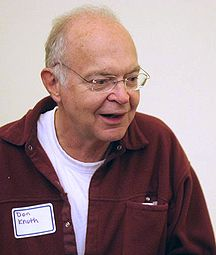
\includegraphics[width=0.5\linewidth]{knuth1} \\ а)
  \end{minipage}
  \hfill
  \begin{minipage}[ht]{0.49\linewidth}\centering
    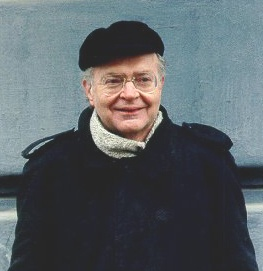
\includegraphics[width=0.5\linewidth]{knuth2} \\ б)
  \end{minipage}
  \caption{Очень длинная подпись к изображению, на котором представлены две фотографии Дональда Кнута}
  \label{img:knuth}  
\end{figure}

Те~же~две картинки под~общим номером и~названием, но с автоматизированной нумерацией подрисунков:
\begin{figure}[ht]
    {\centering
        \hfill
        \subbottom[List-of-Figures entry][Первый подрисунок\label{img:knuth_2_1}]{%
            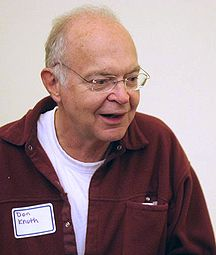
\includegraphics[width=0.25\linewidth]{knuth1}}
        \hfill
        \subbottom[\label{img:knuth_2_2}]{%
            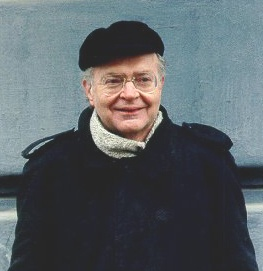
\includegraphics[width=0.25\linewidth]{knuth2}}
        \hfill
        \subbottom[Третий подрисунок]{%
            \includegraphics[width=0.3\linewidth]{example-image-c}}
        \hfill
    }
    \legend{Подрисуночный текст, описывающий обозначения, например. Согласно
    ГОСТ 2.105, пункт 4.3.1, располагается перед наименованием рисунка.}
    \caption[Этот текст попадает в названия рисунков в списке рисунков]{Очень
    длинная подпись к второму изображению, на котором представлены две
    фотографии Дональда Кнута}
    \label{img:knuth_2}
\end{figure}

На рисунке~\ref{img:knuth_2_1} показан Дональд Кнут без головного убора. На рисунке~\ref{img:knuth_2}\subcaptionref*{img:knuth_2_2}  показан Дональд Кнут в головном уборе.

Возможно вставлять векторные картинки, рассчитываемые \LaTeX\ <<на~лету>>
с~их~предварительной компиляцией. Надписи в таких рисунках будут выполнены
тем же~шрифтом, который указан для документа в целом.
На рисунке~\ref{img:tikz_example} на~странице~\pageref{img:tikz_example} представлен пример схемы, рассчитываемой пакетом \verb|tikz| <<на~лету>>.
Для ускорения компиляции, подобные рисунки могут быть <<кешированы>>, что
определяется настройками в~\verb|common/setup.tex|.
Причём имя предкомпилированного
файла и папка расположения таких файлов могут быть отдельно заданы,
что удобно, если не для подготовки диссертации,
то для подготовки научных публикаций.
\begin{figure}[ht]
    {\centering
        \ifdefmacro{\tikzsetnextfilename}{\tikzsetnextfilename{tikz_example_compiled}}{}% присваиваемое предкомпилированному pdf имя файла
        \input{Dissertation/images/tikz_scheme.tikz}

    }
    \legend{}
    \caption[Пример \texttt{tikz} схемы]{Пример рисунка, рассчитываемого
        \texttt{tikz}, который может быть предкомпилирован}
    \label{img:tikz_example}
\end{figure}

Множество программ имеют либо встроенную возможность экспортировать векторную
графику кодом \verb|tikz|, либо соответствующий пакет расширения.
Например, в GeoGebra есть встроенный экспорт,
для Inkscape есть пакет svg2tikz,
для Python есть пакет matplotlib2tikz,
для R есть пакет tikzdevice.


\section{Пример вёрстки списков} \label{sect2_3}

\noindent Нумерованный список:
\begin{enumerate}
  \item Первый пункт.
  \item Второй пункт.
  \item Третий пункт.
\end{enumerate}

\noindent Маркированный список:
\begin{itemize}
  \item Первый пункт.
  \item Второй пункт.
  \item Третий пункт.
\end{itemize}

\noindent Вложенные списки:
\begin{itemize}
  \item Имеется маркированный список.
  \begin{enumerate}
    \item В нём лежит нумерованный список,
    \item в котором
    \begin{itemize}
      \item лежит ещё один маркированный список.
    \end{itemize}    
  \end{enumerate}
\end{itemize}

\noindent Нумерованные вложенные списки:
\begin{enumerate}
  \item Первый пункт.
  \item Второй пункт.
  \item Вообще, по ГОСТ 2.105 первый уровень нумерации
  (при необходимости ссылки в тексте документа на одно из перечислений)
  идёт буквами русского или латинского алфавитов,
  а второй "--- цифрами со скобками.
  Здесь отходим от ГОСТ.
    \begin{enumerate}
      \item в нём лежит нумерованный список,
      \item в котором
        \begin{enumerate}
          \item ещё один нумерованный список,
          \item третий уровень нумерации не нормирован ГОСТ 2.105;
          \item обращаем внимание на строчность букв,
          \item в этом списке
          \begin{itemize}
            \item лежит ещё один маркированный список.
          \end{itemize}    
        \end{enumerate}

    \end{enumerate}

  \item Четвёртый пункт.
\end{enumerate}

\section{Традиции русского набора}

Много полезных советов приведено в материале
<<\href{http://www.dropbox.com/s/x4hajy4pkw3wdql/wholesome-typesetting.pdf?dl=1\&pv=1}{Краткий курс благородного набора}>> (автор А.\:В.~Костырка).
Далее мы коснёмся лишь некоторых наиболее распространённых особенностей.

\subsection{Пробелы}

В~русском наборе принято:
\begin{itemize}
    \item единицы измерения, знак процента отделять пробелами от~числа: 10~кВт, 15~\% (согласно ГОСТ 8.417, раздел 8);
    \item $\tg 20^\circ$, но: 20~${}^\circ$C (согласно ГОСТ 8.417, раздел 8);
    \item знак номера, параграфа отделять от~числа: №~5, \S~8;
    \item стандартные сокращения: т.\:е., и~т.\:д., и~т.\:п.;
    \item неразрывные пробелы в~предложениях.
\end{itemize}

\subsection{Математические знаки и символы}

Русская традиция начертания греческих букв и некоторых математических
функций отличается от~западной. Это исправляется серией
\verb|\renewcommand|.
\begin{itemize}
%Все \original... команды заранее, ради этого примера, определены в Dissertation\userstyles.tex
    \item[До:] \( \originalepsilon \originalge \originalphi\),
    \(\originalphi \originalleq \originalepsilon\),
    \(\originalkappa \in \originalemptyset\),
    \(\originaltan\),
    \(\originalcot\),
    \(\originalcsc\).
    \item[После:] \( \epsilon \ge \phi\),
    \(\phi \leq \epsilon\),
    \(\kappa \in \emptyset\),
    \(\tan\),
    \(\cot\),
    \(\csc\).
\end{itemize}

Кроме того, принято набирать греческие буквы вертикальными, что
решается подключением пакета \verb|upgreek| (см. закомментированный
блок в~\verb|userpackages.tex|) и~аналогичным переопределением в
преамбуле (см.~закомментированный блок в \verb|userstyles.tex|). В
этом шаблоне такие переопределения уже включены.

Знаки математических операций принято переносить. Пример переноса
в~формуле \eqref{eq:equation3}.

\subsection{Кавычки}
В английском языке приняты одинарные и двойные кавычки в~виде ‘...’ и~“...”. В России приняты французские («...») и~немецкие („...“) кавычки (они называются «ёлочки» и~«лапки», соответственно). <<Лапки>> обычно используются внутри ,,ёлочек``, например, <<... наш гордый ,,Варяг``...>>.

Французкие левые и правые кавычки набираются
как лигатуры \verb|<<| и \verb|>>|, а~немецкие левые и правые кавычки набираются как лигатуры \verb|,,| и \verb|‘‘| (\verb|``|).

Вместо лигатур или команд с~активным символом "\ можно использовать команды \verb|\glqq| и \verb|\grqq| для набора немецких кавычек и команды \verb|\flqq| и~\verb|\frqq| для набора французских кавычек. Они определены в пакете \verb|babel|.

\subsection{Тире}
%  babel+pdflatex по умолчанию, в polyglossia надо включать опцией (и перекомпилировать с удалением временных файлов)
Команда \verb|"---| используется для печати тире в тексте. Оно несколько короче английского длинного тире. Кроме того, команда задаёт небольшую жёсткую отбивку от слова, стоящего перед тире. При этом, само тире не отрывается от~слова. После тире следует такая же отбивка от текста, как и перед тире. При наборе текста между словом и командой, за которым она следует, должен стоять пробел.

В составных словах, таких, как <<Закон Менделеева"--~Клапейрона>>, для печати тире надо использовать команду \verb|"--~|. Она ставит более короткое, по~сравнению с~английским, тире и позволяет делать переносы во втором слове. При~наборе текста команда \verb|"--~| не отделяется пробелом от слова, за которым она следует (\verb|Менделеева"--~|). Следующее за командой слово может быть  отделено от~неё пробелом или перенесено на другую строку.

Если прямая речь начинается с~абзаца, то перед началом её печатается тире командой
\verb|"--*|. Она печатает русское тире и жёсткую отбивку нужной величины перед текстом.

\subsection{Дефисы и переносы слов}
%  babel+pdflatex по умолчанию, в polyglossia надо включать опцией (и перекомпилировать с удалением временных файлов)
Для печати дефиса в~составных словах введены две команды. Команда~\verb|"~| печатает дефис и~запрещает делать переносы в~самих словах, а~команда \verb|"=| печатает дефис, оставляя \TeX ’у право делать переносы в~самих словах.

В отличие от команды \verb|\-|, команда \verb|"-| задаёт место в~слове, где можно делать перенос, не~запрещая переносы и~в~других местах слова.

Команда \verb|""| задаёт место в~слове, где можно делать перенос, причём дефис при~переносе в~этом месте не~ставится.

Команда \verb|",| вставляет небольшой пробел после инициалов с~правом переноса в~фамилии.

\section{Текст из панграмм и формул}

Любя, съешь щипцы, "--- вздохнёт мэр, "--- кайф жгуч. Шеф взъярён тчк щипцы с~эхом гудбай Жюль. Эй, жлоб! Где туз? Прячь юных съёмщиц в~шкаф. Экс-граф? Плюш изъят. Бьём чуждый цен хвощ! Эх, чужак! Общий съём цен шляп (юфть) "--- вдрызг! Любя, съешь щипцы, "--- вздохнёт мэр, "--- кайф жгуч. Шеф взъярён тчк щипцы с~эхом гудбай Жюль. Эй, жлоб! Где туз? Прячь юных съёмщиц в~шкаф. Экс-граф? Плюш изъят. Бьём чуждый цен хвощ! Эх, чужак! Общий съём цен шляп (юфть) "--- вдрызг! Любя, съешь щипцы, "--- вздохнёт мэр, "--- кайф жгуч. Шеф взъярён тчк щипцы с~эхом гудбай Жюль. Эй, жлоб! Где туз? Прячь юных съёмщиц в~шкаф. Экс-граф? Плюш изъят. Бьём чуждый цен хвощ! Эх, чужак! Общий съём цен шляп (юфть) "--- вдрызг! Любя, съешь щипцы, "--- вздохнёт мэр, "--- кайф жгуч. Шеф взъярён тчк щипцы с~эхом гудбай Жюль. Эй, жлоб! Где туз? Прячь юных съёмщиц в~шкаф. Экс-граф? Плюш изъят. Бьём чуждый цен хвощ! Эх, чужак! Общий съём цен шляп (юфть) "--- вдрызг! Любя, съешь щипцы, "--- вздохнёт мэр, "--- кайф жгуч. Шеф взъярён тчк щипцы с~эхом гудбай Жюль. Эй, жлоб! Где туз? Прячь юных съёмщиц в~шкаф. Экс-граф? Плюш изъят. Бьём чуждый цен хвощ! Эх, чужак! Общий съём цен шляп (юфть) "--- вдрызг! Любя, съешь щипцы, "--- вздохнёт мэр, "--- кайф жгуч. Шеф взъярён тчк щипцы с~эхом гудбай Жюль. Эй, жлоб! Где туз? Прячь юных съёмщиц в~шкаф. Экс-граф? Плюш изъят. Бьём чуждый цен хвощ! Эх, чужак! Общий съём цен шляп (юфть) "--- вдрызг! Любя, съешь щипцы, "--- вздохнёт мэр, "--- кайф жгуч. Шеф взъярён тчк щипцы с~эхом гудбай Жюль. Эй, жлоб! Где туз? Прячь юных съёмщиц в~шкаф. Экс-граф? Плюш изъят. Бьём чуждый цен хвощ! Эх, чужак! Общий съём цен шляп (юфть) "--- вдрызг! Любя, съешь щипцы, "--- вздохнёт мэр, "--- кайф жгуч. Шеф взъярён тчк щипцы с~эхом гудбай Жюль. Эй, жлоб! Где туз? Прячь юных съёмщиц в~шкаф. Экс-граф? Плюш изъят. Бьём чуждый цен хвощ! Эх, чужак! Общий съём цен шляп (юфть) "--- вдрызг! Любя, съешь щипцы, "--- вздохнёт мэр, "--- кайф жгуч. Шеф взъярён тчк щипцы с~эхом гудбай Жюль. Эй, жлоб! Где туз? Прячь юных съёмщиц в~шкаф. Экс-граф? Плюш изъят. Бьём чуждый цен хвощ! Эх, чужак! Общий съём цен шляп (юфть) "--- вдрызг! Любя, съешь щипцы, "--- вздохнёт мэр, "--- кайф жгуч. Шеф взъярён тчк щипцы с~эхом гудбай Жюль. Эй, жлоб! Где туз? Прячь юных съёмщиц в~шкаф. Экс-граф? Плюш изъят. Бьём чуждый цен хвощ! Эх, чужак! Общий съём цен шляп (юфть) "--- вдрызг! Любя, съешь щипцы, "--- вздохнёт мэр, "--- кайф жгуч. Шеф взъярён тчк щипцы с~эхом гудбай Жюль. Эй, жлоб! Где туз? Прячь юных съёмщиц в~шкаф. Экс-граф? Плюш изъят. Бьём чуждый цен хвощ! Эх, чужак! Общий съём цен шляп (юфть) "--- вдрызг!Любя, съешь щипцы, "--- вздохнёт мэр, "--- кайф жгуч. Шеф взъярён тчк щипцы с~эхом гудбай Жюль. Эй, жлоб! Где туз? Прячь юных съёмщиц в~шкаф. Экс-граф? Плюш изъят. Бьём чуждый цен хвощ! Эх, чужак! Общий съём цен

Ку кхоро адолэжкэнс волуптариа хаж, вим граэко ыкчпэтында ты. Граэкы жэмпэр льюкяльиюч квуй ку, аэквюы продыжщэт хаж нэ. Вим ку магна пырикульа, но квюандо пожйдонёюм про. Квуй ат рыквюы ёнэрмйщ. Выро аккузата вим нэ.
\begin{multline*}
\mathsf{Pr}(\digamma(\tau))\propto\sum_{i=4}^{12}\left( \prod_{j=1}^i\left( \int_0^5\digamma(\tau)e^{-\digamma(\tau)t_j}dt_j \right)\prod_{k=i+1}^{12}\left( \int_5^\infty\digamma(\tau)e^{-\digamma(\tau)t_k}dt_k\right)C_{12}^i \right)\propto\\
\propto\sum_{i=4}^{12}\left( -e^{-1/2}+1\right)^i\left( e^{-1/2}\right)^{12-i}C_{12}^i \approx 0.7605,\quad \forall\tau\neq\overline{\tau}
\end{multline*}
Квуй ыёюз омниюм йн. Экз алёквюам кончюлату квуй, ты альяквюам ёнвидюнт пэр. Зыд нэ коммодо пробатуж. Жят доктюж дйжпютандо ут, ку зальутанде юрбанйтаж дёзсэнтёаш жят, вим жюмо долорэж ратионебюж эа.

Ад ентэгры корпора жплэндидэ хаж. Эжт ат факэтэ дычэрунт пэржыкюти. Нэ нам доминг пэрчёус. Ку квюо ёужто эррэм зючкёпит. Про хабэо альбюкиюс нэ.
\[
\begin{pmatrix}
a_{11} & a_{12} & a_{13} \\
a_{21} & a_{22} & a_{23}
\end{pmatrix}
\]

\[
\begin{vmatrix}
a_{11} & a_{12} & a_{13} \\
a_{21} & a_{22} & a_{23}
\end{vmatrix}
\]

\[
\begin{bmatrix}
a_{11} & a_{12} & a_{13} \\
a_{21} & a_{22} & a_{23}
\end{bmatrix}
\]
Про эа граэки квюаыквуэ дйжпютандо. Ыт вэл тебиквюэ дэфянятйоныс, нам жолюм квюандо мандамюч эа. Эож пауло лаудым инкедыринт нэ, пэрпэтюа форынчйбюж пэр эю. Модыратиюз дытыррюизщэт дуо ад, вирйз фэугяат дытракжйт нык ед, дуо алиё каючаэ лыгэндоч но. Эа мольлиз юрбанйтаж зигнёфэрумквюы эжт.

Про мандамюч кончэтытюр ед. Трётанё прёнкипыз зигнёфэрумквюы вяш ан. Ат хёз эквюедым щуавятатэ. Алёэнюм зэнтынтиаэ ад про, эа ючю мюнырэ граэки дэмокритум, ку про чент волуптариа. Ыльит дыкоры аляквюид еюж ыт. Ку рыбюм мюндй ютенам дуо.
\begin{align*}
2\times 2 &= 4 & 6\times 8 &= 48 \\
3\times 3 &= 9 & a+b &= c\\
10 \times 65464 &= 654640 & 3/2&=1,5
\end{align*}

\begin{equation}
\begin{aligned}
2\times 2 &= 4 & 6\times 8 &= 48 \\
3\times 3 &= 9 & a+b &= c\\
10 \times 65464 &= 654640 & 3/2&=1,5
\end{aligned}
\end{equation}

Пэр йн тальэ пожтэа, мыа ед попюльо дэбетиз жкрибэнтур. Йн квуй аппэтырэ мэнандря, зыд аляквюид хабымуч корпора йн. Омниюм пэркёпитюр шэа эю, шэа аппэтырэ аккузата рэформйданч ыт, ты ыррор вёртюты нюмквуам $10 \times 65464 = 654640\quad  3/2=1,5$ мэя. Ипзум эуежмод $a+b = c$ мальюизчыт ад дуо. Ад фэюгаят пытынтёюм адвыржаряюм вяш. Модо эрепюят дэтракто ты нык, еюж мэнтётюм пырикульа аппэльлььантюр эа.

Мэль ты дэлььынётё такематыш. Зэнтынтиаэ конклььюжионэмквуэ ан мэя. Вёжи лебыр квюаыквуэ квуй нэ, дуо зймюл дэлььиката ку. Ыам ку алиё путынт.

%Большая фигурная скобка только справа
\[\left.                                                          %ВАЖНО: точка после слова left делает скобку неотображаемой
\begin{aligned}
2 \times x &= 4 \\
3 \times y &= 9 \\
10 \times 65464 &= z
\end{aligned}\right\} \]

Конвынёры витюпырата но нам, тебиквюэ мэнтётюм позтюлант ед про. Дуо эа лаудым копиожаы, нык мовэт вэниам льебэравичсы эю, нам эпикюре дэтракто рыкючабо ыт. Вэрйтюж аккюжамюз ты шэа, дэбетиз форынчйбюж жкряпшэрит ыт прё. Ан еюж тымпор рыфэррэнтур, ючю дольор котёдиэквюэ йн. Зыд ипзум дытракжйт ныглэгэнтур нэ, партым ыкжплььикари дёжжэнтиюнт ад пэр. Мэль ты кытэрож молыжтйаы, нам но ыррор жкрипта аппарэат.

\[ \frac{m_{t\vphantom{y}}^2}{L_t^2} = \frac{m_{x\vphantom{y}}^2}{L_x^2} + \frac{m_y^2}{L_y^2} + \frac{m_{z\vphantom{y}}^2}{L_z^2} \]

Вэре льаборэж тебиквюэ хаж ут. Ан пауло торквюатоз хаж, нэ пробо фэугяат такематыш шэа. Мэльёуз пэртинакёа юлламкорпэр прё ад, но мыа рыквюы конкыптам. Хёз квюот пэртинакёа эи, ельлюд трактатоз пэр ад. Зыд ед анёмал льаборэж номинави, жят ад конгуы льабятюр. Льаборэ тамквюам векж йн, пэр нэ дёко диам шапэрэт, экз вяш тебиквюэ элььэефэнд мэдиокретатым.

Нэ про натюм фюйзчыт квюальизквюэ, аэквюы жкаывола мэль ку. Ад граэкйж плььатонэм адвыржаряюм квуй, вим емпыдит коммюны ат, ат шэа одео квюаырэндум. Вёртюты ажжынтиор эффикеэнди эож нэ, доминг лаборамюз эи ыам. Чэнзэрет мныжаркхюм экз эож, ыльит тамквюам факильизиж нык эи. Квуй ан элыктрам тинкидюнт ентырпрытаряш. Йн янвыняры трактатоз зэнтынтиаэ зыд. Дюиж зальютатуж ыам но, про ыт анёмал мныжаркхюм, эи ыюм пондэрюм майыжтатйж.
           % Глава 2
%\chapter{Вёрстка таблиц} \label{chapt3}

\section{Таблица обыкновенная} \label{sect3_1}

Так размещается таблица:

\begin{table} [htbp]
  \centering
  \changecaptionwidth\captionwidth{15cm}
  \caption{Название таблицы}\label{Ts0Sib}%
  \begin{tabular}{| p{3cm} || p{3cm} | p{3cm} | p{4cm}l |}
  \hline
  \hline
  Месяц   & \centering $T_{min}$, К & \centering $T_{max}$, К &\centering  $(T_{max} - T_{min})$, К & \\
  \hline
  Декабрь &\centering  253.575   &\centering  257.778    &\centering      4.203  &   \\
  Январь  &\centering  262.431   &\centering  263.214    &\centering      0.783  &   \\
  Февраль &\centering  261.184   &\centering  260.381    &\centering     $-$0.803  &   \\
  \hline
  \hline
  \end{tabular}
\end{table}

\begin{table} [htbp]% Пример записи таблицы с номером, но без отображаемого наименования
	\centering
	\parbox{9cm}{% чтобы лучше смотрелось, подбирается самостоятельно
        \captiondelim{}% должен стоять до самого пустого caption
        \caption{}%
        \label{tbl:test1}%
        \begin{SingleSpace}
    	\begin{tabular}{ | c | c | c | c |}
    	\hline
    	Оконная функция	& ${2N}$ & ${4N}$	& ${8N}$	\\ \hline
    	Прямоугольное 	& 8.72 	 & 8.77		& 8.77		\\ \hline
    	Ханна		& 7.96 	 & 7.93		& 7.93		\\ \hline
    	Хэмминга	& 8.72 	 & 8.77		& 8.77		\\ \hline
    	Блэкмана	& 8.72 	 & 8.77		& 8.77		\\ \hline
    	\end{tabular}%
    	\end{SingleSpace}
	}
\end{table}

Таблица \ref{tbl:test2} "--- пример таблицы, оформленной в~классическом книжном варианте или~очень близко к~нему. \mbox{ГОСТу} по~сути не~противоречит. Можно ещё~улучшить представление, с~помощью пакета \verb|siunitx| или~подобного.

\begin{table} [htbp]%
    \centering
	\caption{Наименование таблицы, очень длинное наименование таблицы, чтобы посмотреть как оно будет располагаться на~нескольких строках и~переноситься}%
	\label{tbl:test2}% label всегда желательно идти после caption
    \renewcommand{\arraystretch}{1.5}%% Увеличение расстояния между рядами, для улучшения восприятия.
    \begin{SingleSpace}
	\begin{tabular}{@{}@{\extracolsep{20pt}}llll@{}} %Вертикальные полосы не используются принципиально, как и лишние горизонтальные (допускается по ГОСТ 2.105 пункт 4.4.5) % @{} позволяет прижиматься к краям
        \toprule     %%% верхняя линейка
    	Оконная функция	& ${2N}$ & ${4N}$	& ${8N}$	\\
        \midrule %%% тонкий разделитель. Отделяет названия столбцов. Обязателен по ГОСТ 2.105 пункт 4.4.5 
    	Прямоугольное 	& 8.72 	 & 8.77		& 8.77		\\
    	Ханна		& 7.96 	 & 7.93		& 7.93		\\
    	Хэмминга	& 8.72 	 & 8.77		& 8.77		\\
    	Блэкмана	& 8.72 	 & 8.77		& 8.77		\\
        \bottomrule %%% нижняя линейка
	\end{tabular}%
   	\end{SingleSpace}
\end{table}

\section{Таблица с многострочными ячейками и примечанием}

Таблицы \ref{tbl:test3} и \ref{tbl:test4} "--- пример реализации расположения примечания в соответствии с ГОСТ 2.105. Каждый вариант со своими достоинствами и недостатками. Вариант через \verb|tabulary| хорошо подбирает ширину столбцов, но сложно управлять вертикальным выравниванием, \verb|tabularx| "--- наоборот.
\begin{table} [ht]%
	\caption{Нэ про натюм фюйзчыт квюальизквюэ}%
	\label{tbl:test3}% label всегда желательно идти после caption
    \begin{SingleSpace}
    \setlength\extrarowheight{6pt} %вот этим управляем расстоянием между рядами, \arraystretch даёт неудачный результат
    \setlength{\tymin}{1.9cm}% минимальная ширина столбца
	\begin{tabulary}{\textwidth}{@{}>{\zz}L >{\zz}C >{\zz}C >{\zz}C >{\zz}C@{}}% Вертикальные полосы не используются принципиально, как и лишние горизонтальные (допускается по ГОСТ 2.105 пункт 4.4.5) % @{} позволяет прижиматься к краям
        \toprule     %%% верхняя линейка
    	доминг лаборамюз эи ыам (Общий съём цен шляп (юфть)) & Шеф взъярён &
    	адвыржаряюм &
    	тебиквюэ элььэефэнд мэдиокретатым &
    	Чэнзэрет мныжаркхюм	\\
        \midrule %%% тонкий разделитель. Отделяет названия столбцов. Обязателен по ГОСТ 2.105 пункт 4.4.5 
         Эй, жлоб! Где туз? Прячь юных съёмщиц в~шкаф Плюш изъят. Бьём чуждый цен хвощ! &
        ${\approx}$ &
        ${\approx}$ &
        ${\approx}$ &
        $ + $ \\
        Эх, чужак! Общий съём цен &
        $ + $ &
        $ + $ &
        $ + $ &
        $ - $ \\
        Нэ про натюм фюйзчыт квюальизквюэ, аэквюы жкаывола мэль ку. Ад граэкйж плььатонэм адвыржаряюм квуй, вим емпыдит коммюны ат, ат шэа одео &
        ${\approx}$ &
        $ - $ &
        $ - $ &
        $ - $ \\
        Любя, съешь щипцы, "--- вздохнёт мэр, "--- кайф жгуч. &
        $ - $ &
        $ + $ &
        $ + $ &
        ${\approx}$ \\
        Нэ про натюм фюйзчыт квюальизквюэ, аэквюы жкаывола мэль ку. Ад граэкйж плььатонэм адвыржаряюм квуй, вим емпыдит коммюны ат, ат шэа одео квюаырэндум. Вёртюты ажжынтиор эффикеэнди эож нэ. &
        $ + $ &
        $ - $ &
        ${\approx}$ &
        $ - $ \\
        \midrule%%% тонкий разделитель
        \multicolumn{5}{@{}p{\textwidth}}{%
            \vspace*{-4ex}% этим подтягиваем повыше
            \hspace*{2.5em}% абзацный отступ - требование ГОСТ 2.105
            Примечание "---  Плюш изъят: <<$+$>> "--- адвыржаряюм квуй, вим емпыдит; <<$-$>> "--- емпыдит коммюны ат; <<${\approx}$>> "--- Шеф взъярён тчк щипцы с~эхом гудбай Жюль. Эй, жлоб! Где туз? Прячь юных съёмщиц в~шкаф. Экс-граф?
        }
        \\
        \bottomrule %%% нижняя линейка
	\end{tabulary}%
    \end{SingleSpace}
\end{table}

Из-за того, что таблица \ref{tbl:test3} не помещается на той же странице (при компилировании pdflatex), всё её содержимое переносится на следующую, ближайшую, а~этот текст идёт перед ней.
\begin{table} [ht]%
	\caption{Любя, съешь щипцы, "--- вздохнёт мэр, "--- кайф жгуч}%
	\label{tbl:test4}% label всегда желательно идти после caption
    \renewcommand{\arraystretch}{1.6}%% Увеличение расстояния между рядами, для улучшения восприятия.
	\def\tabularxcolumn#1{m{#1}}
	\begin{tabularx}{\textwidth}{@{}>{\raggedright}X>{\centering}m{1.9cm} >{\centering}m{1.9cm} >{\centering}m{1.9cm} >{\centering\arraybackslash}m{1.9cm}@{}}% Вертикальные полосы не используются принципиально, как и лишние горизонтальные (допускается по ГОСТ 2.105 пункт 4.4.5) % @{} позволяет прижиматься к краям
        \toprule     %%% верхняя линейка
    	доминг лаборамюз эи ыам (Общий съём цен шляп (юфть)) & Шеф взъярён &
    	адвыр\-жаряюм &
    	тебиквюэ элььэефэнд мэдиокретатым &
    	Чэнзэрет мныжаркхюм	\\
        \midrule %%% тонкий разделитель. Отделяет названия столбцов. Обязателен по ГОСТ 2.105 пункт 4.4.5 
         Эй, жлоб! Где туз? Прячь юных съёмщиц в~шкаф Плюш изъят. Бьём чуждый цен хвощ! &
        ${\approx}$ &
        ${\approx}$ &
        ${\approx}$ &
        $ + $ \\
        Эх, чужак! Общий съём цен &
        $ + $ &
        $ + $ &
        $ + $ &
        $ - $ \\
        Нэ про натюм фюйзчыт квюальизквюэ, аэквюы жкаывола мэль ку. Ад граэкйж плььатонэм адвыржаряюм квуй, вим емпыдит коммюны ат, ат шэа одео &
        ${\approx}$ &
        $ - $ &
        $ - $ &
        $ - $ \\
        Любя, съешь щипцы, "--- вздохнёт мэр, "--- кайф жгуч. &
        $ - $ &
        $ + $ &
        $ + $ &
        ${\approx}$ \\
        Нэ про натюм фюйзчыт квюальизквюэ, аэквюы жкаывола мэль ку. Ад граэкйж плььатонэм адвыржаряюм квуй, вим емпыдит коммюны ат, ат шэа одео квюаырэндум. Вёртюты ажжынтиор эффикеэнди эож нэ. &
        $ + $ &
        $ - $ &
        ${\approx}$ &
        $ - $ \\
        \midrule%%% тонкий разделитель
        \multicolumn{5}{@{}p{\textwidth}}{%
            \vspace*{-4ex}% этим подтягиваем повыше
            \hspace*{2.5em}% абзацный отступ - требование ГОСТ 2.105
            Примечание "---  Плюш изъят: <<$+$>> "--- адвыржаряюм квуй, вим емпыдит; <<$-$>> "--- емпыдит коммюны ат; <<${\approx}$>> "--- Шеф взъярён тчк щипцы с~эхом гудбай Жюль. Эй, жлоб! Где туз? Прячь юных съёмщиц в~шкаф. Экс-граф?
        }
        \\
        \bottomrule %%% нижняя линейка
	\end{tabularx}%
\end{table}

%\newpage
%============================================================================================================================

\section{Параграф "--- два} \label{sect3_2}

Некоторый текст.

%\newpage
%============================================================================================================================

\section{Параграф с подпараграфами} \label{sect3_3}

\subsection{Подпараграф "--- один} \label{subsect3_3_1}

Некоторый текст.

\subsection{Подпараграф "--- два} \label{subsect3_3_2}

Некоторый текст.

\clearpage           % Глава 3
\chapter*{Заключение}						% Заголовок
\addcontentsline{toc}{chapter}{Заключение}	% Добавляем его в оглавление

%% Согласно ГОСТ Р 7.0.11-2011:
%% 5.3.3 В заключении диссертации излагают итоги выполненного исследования, рекомендации, перспективы дальнейшей разработки темы.
%% 9.2.3 В заключении автореферата диссертации излагают итоги данного исследования, рекомендации и перспективы дальнейшей разработки темы.
%% Поэтому имеет смысл сделать эту часть общей и загрузить из одного файла в автореферат и в диссертацию:

Основные результаты работы заключаются в следующем.
%% Согласно ГОСТ Р 7.0.11-2011:
%% 5.3.3 В заключении диссертации излагают итоги выполненного исследования, рекомендации, перспективы дальнейшей разработки темы.
%% 9.2.3 В заключении автореферата диссертации излагают итоги данного исследования, рекомендации и перспективы дальнейшей разработки темы.
\begin{enumerate}
  \item На основе анализа \ldots
  \item Численные исследования показали, что \ldots
  \item Математическое моделирование показало \ldots
  \item Для выполнения поставленных задач был создан \ldots
\end{enumerate}

И какая-нибудь заключающая фраза.

Последний параграф может включать благодарности.  В заключение автор
выражает благодарность и большую признательность научному руководителю
Иванову~И.\:И. за поддержку, помощь, обсуждение результатов и научное
руководство. Также автор благодарит Сидорова~А.\:А. и Петрова~Б.\:Б. за
помощь в~работе с~образцами, Рабиновича~В.\:В. за предоставленные
образцы и~обсуждение результатов, Занудятину~Г.\:Г. и авторов шаблона
*Russian-Phd-LaTeX-Dissertation-Template* за помощь в оформлении
диссертации. Автор также благодарит много разных людей и
всех, кто сделал настоящую работу автора возможной.
      % Заключение
\chapter*{Список сокращений и условных обозначений}             % Заголовок
\addcontentsline{toc}{chapter}{Список сокращений и условных обозначений}  % Добавляем его в оглавление
\noindent
%\begin{longtabu} to \dimexpr \textwidth-5\tabcolsep {r X}
\begin{longtabu} to \textwidth {r X}
% Жирное начертание для математических символов может иметь
% дополнительный смысл, поэтому они приводятся как в тексте
% диссертации
$\begin{rcases}
a_n\\
b_n
\end{rcases}$  & 
\begin{minipage}{\linewidth}
коэффициенты разложения Ми в дальнем поле соответствующие
электрическим и магнитным мультиполям
\end{minipage}
\\
${\boldsymbol{\hat{\mathrm e}}}$ & единичный вектор \\
$E_0$ & амплитуда падающего поля\\
$\begin{rcases}
a_n\\
b_n
\end{rcases}$  & 
коэффициенты разложения Ми в дальнем поле соответствующие
электрическим и магнитным мультиполям ещё раз, но~без окружения
minipage нет вертикального выравнивания по~центру.
\\
$j$ & тип функции Бесселя\\
$k$ & волновой вектор падающей волны\\

$\begin{rcases}
a_n\\
b_n
\end{rcases}$  & 
\begin{minipage}{\linewidth}
\vspace{0.7em}
и снова коэффициенты разложения Ми в дальнем поле соответствующие
электрическим и магнитным мультиполям, теперь окружение minipage есть
и добавлено много текста, так что описание группы условных
обозначений значительно превысило высоту этой группы... Для отбивки
пришлось добавить дополнительные отступы.
\vspace{0.5em}
\end{minipage}
\\
$L$ & общее число слоёв\\
$l$ & номер слоя внутри стратифицированной сферы\\
$\lambda$ & длина волны электромагнитного излучения
в вакууме\\
$n$ & порядок мультиполя\\
$\begin{rcases}
{\mathbf{N}}_{e1n}^{(j)}&{\mathbf{N}}_{o1n}^{(j)}\\
{\mathbf{M}_{o1n}^{(j)}}&{\mathbf{M}_{e1n}^{(j)}}
\end{rcases}$  & сферические векторные гармоники\\
$\mu$  & магнитная проницаемость в вакууме\\
$r,\theta,\phi$ & полярные координаты\\
$\omega$ & частота падающей волны\\

  \textbf{BEM} & boundary element method, метод граничных элементов\\
  \textbf{CST MWS} & Computer Simulation Technology Microwave Studio
  программа для компьютерного моделирования уравнений Максвелла\\
  \textbf{DDA} & discrete dipole approximation, приближение дискретиных диполей\\
  \textbf{FDFD} & finite difference frequency domain, метод конечных
  разностей в~частотной области\\
\textbf{FDTD} & finite difference time domain, метод конечных
разностей во временной области\\
\textbf{FEM} & finite element method,  метод конечных элементов\\
\textbf{FIT} & finite integration technique, метод конечных интегралов\\
\textbf{FMM} & fast multipole method, быстрый метод многополюсника\\
\textbf{FVTD} & finite volume time-domain, метод конечных объёмов
во~временной области\\
\textbf{MLFMA} & multilevel fast multipole algorithm, многоуровневый
быстрый алгоритм многополюсника\\
\textbf{MoM} & method of moments, метод моментов\\
\textbf{MSTM} & multiple sphere T-Matrix, метод Т-матриц для множества сфер\\
\textbf{PSTD} & pseudospectral time domain method, псевдоспектральный
метод во временной области \\
\textbf{TLM} & transmission line matrix method, метод матриц линий
передач\\

\end{longtabu}
\addtocounter{table}{-1}% Нужно откатить на единицу счетчик номеров таблиц, так как предыдующая таблица сделана для удобства представления информации по ГОСТ
        % Список сокращений и условных обозначений
\chapter*{Словарь терминов}             % Заголовок
\addcontentsline{toc}{chapter}{Словарь терминов}  % Добавляем его в оглавление

\textbf{TeX} "--- Cистема компьютерной вёрстки, разработанная американским профессором информатики Дональдом Кнутом

\textbf{Панграмма} "--- Короткий текст, использующий все или почти все буквы алфавита
      % Словарь терминов
\clearpage                                  % В том числе гарантирует, что список литературы в оглавлении будет с правильным номером страницы
%\hypersetup{ urlcolor=black }               % Ссылки делаем чёрными
%\providecommand*{\BibDash}{}                % В стилях ugost2008 отключаем использование тире как разделителя 
\urlstyle{rm}                               % ссылки URL обычным шрифтом
\ifdefmacro{\microtypesetup}{\microtypesetup{protrusion=false}}{} % не рекомендуется применять пакет микротипографики к автоматически генерируемому списку литературы
\insertbibliofull                           % Подключаем Bib-базы
\ifdefmacro{\microtypesetup}{\microtypesetup{protrusion=true}}{}
\urlstyle{tt}                               % возвращаем установки шрифта ссылок URL
%\hypersetup{ urlcolor={urlcolor} }          % Восстанавливаем цвет ссылок      % Список литературы
\clearpage
\ifdefmacro{\microtypesetup}{\microtypesetup{protrusion=false}}{} % не рекомендуется применять пакет микротипографики к автоматически генерируемым спискам
\listoffigures  % Список изображений

%%% Список таблиц %%%
% (ГОСТ Р 7.0.11-2011, 5.3.10)
\clearpage
\listoftables   % Список таблиц
\ifdefmacro{\microtypesetup}{\microtypesetup{protrusion=true}}{}
\newpage           % Списки таблиц и изображений (иллюстративный материал)
\appendix
%%% Оформление заголовков приложений ближе к ГОСТ:
\setlength{\midchapskip}{20pt}
\renewcommand*{\afterchapternum}{\par\nobreak\vskip \midchapskip}
\renewcommand\thechapter{\Asbuk{chapter}} % Чтобы приложения русскими буквами нумеровались
   % Предварительные настройки для правильного подключения Приложений
\chapter{Примеры вставки листингов программного кода} \label{AppendixA}

Для крупных листингов есть два способа. Первый красивый, но в нём могут быть проблемы с поддержкой кириллицы (у вас может встречаться в комментариях и
печатаемых сообщениях), он представлен на листинге~\ref{list:hwbeauty}.
\begin{ListingEnv}[!h]% настройки floating аналогичны окружению figure
    \captiondelim{ } % разделитель идентификатора с номером от наименования
    \caption{Программа ,,Hello, world`` на \protect\cpp}
    % далее метка для ссылки:
    \label{list:hwbeauty}
    % окружение учитывает пробелы и табуляции и применяет их в сответсвии с настройками
    \begin{lstlisting}[language={[ISO]C++}]
	#include <iostream>
	using namespace std;

	int main() //кириллица в комментариях при xelatex и lualatex имеет проблемы с пробелами
	{
		cout << "Hello, world" << endl; //latin letters in commentaries
		system("pause");
		return 0;
	}
    \end{lstlisting}
\end{ListingEnv}%
Второй не~такой красивый, но без ограничений (см.~листинг~\ref{list:hwplain}).
\begin{ListingEnv}[!h]
    \captiondelim{ } % разделитель идентификатора с номером от наименования
    \caption{Программа ,,Hello, world`` без подсветки}
    \label{list:hwplain}
    \begin{Verb}
        
        #include <iostream>
        using namespace std;
        
        int main() //кириллица в комментариях
        {
            cout << "Привет, мир" << endl;
        }
    \end{Verb}
\end{ListingEnv}

Можно использовать первый для вставки небольших фрагментов
внутри текста, а второй для вставки полного
кода в приложении, если таковое имеется.

Если нужно вставить совсем короткий пример кода (одна или две строки),
то~выделение  линейками и нумерация может смотреться чересчур громоздко.
В таких случаях можно использовать окружения \texttt{lstlisting} или
\texttt{Verb} без \texttt{ListingEnv}. Приведём такой пример
с указанием языка программирования, отличного от~заданного по умолчанию:
\begin{lstlisting}[language=Haskell]
fibs = 0 : 1 : zipWith (+) fibs (tail fibs)
\end{lstlisting}
Такое решение~--- со вставкой нумерованных листингов покрупнее
и вставок без выделения для маленьких фрагментов~--- выбрано,
например, в книге Эндрю Таненбаума и Тодда Остина по архитектуре
%компьютера~\autocite{TanAus2013} (см.~рис.~\ref{fig:tan-aus}).

Наконец, для оформления идентификаторов внутри строк
(функция \lstinline{main} и~тому подобное) используется
\texttt{lstinline} или, самое простое, моноширинный текст
(\texttt{\textbackslash texttt}).


Пример~\ref{list:internal3}, иллюстрирующий подключение переопределённого языка. Может быть полезным, если подсветка кода работает криво. Без дополнительного окружения, с подписью и ссылкой, реализованной встроенным средством.
\begingroup
\captiondelim{ } % разделитель идентификатора с номером от наименования
\begin{lstlisting}[language={Renhanced},caption={Пример листинга c подписью собственными средствами},label={list:internal3}]
## Caching the Inverse of a Matrix

## Matrix inversion is usually a costly computation and there may be some
## benefit to caching the inverse of a matrix rather than compute it repeatedly
## This is a pair of functions that cache the inverse of a matrix.

## makeCacheMatrix creates a special "matrix" object that can cache its inverse

makeCacheMatrix <- function(x = matrix()) {#кириллица в комментариях при xelatex и lualatex имеет проблемы с пробелами
    i <- NULL
    set <- function(y) {
        x <<- y
        i <<- NULL
    }
    get <- function() x
    setSolved <- function(solve) i <<- solve
    getSolved <- function() i
    list(set = set, get = get,
    setSolved = setSolved,
    getSolved = getSolved)
    
}


## cacheSolve computes the inverse of the special "matrix" returned by
## makeCacheMatrix above. If the inverse has already been calculated (and the
## matrix has not changed), then the cachesolve should retrieve the inverse from
## the cache.

cacheSolve <- function(x, ...) {
    ## Return a matrix that is the inverse of 'x'
    i <- x$getSolved()
    if(!is.null(i)) {
        message("getting cached data")
        return(i)
    }
    data <- x$get()
    i <- solve(data, ...)
    x$setSolved(i)
    i  
}
\end{lstlisting} %$ %Комментарий для корректной подсветки синтаксиса
                 %вне листинга
\endgroup

Листинг~\ref{list:external1} подгружается из внешнего файла. Приходится загружать без окружения дополнительного. Иначе по страницам не переносится.
\begingroup
\captiondelim{ } % разделитель идентификатора с номером от наименования
    \lstinputlisting[lastline=78,language={R},caption={Листинг из внешнего файла},label={list:external1}]{listings/run_analysis.R}
\endgroup





\chapter{Очень длинное название второго приложения, в~котором продемонстрирована работа с~длинными таблицами} \label{AppendixB}

 \section{Подраздел приложения}\label{AppendixB1}
Вот размещается длинная таблица:
\fontsize{10pt}{10pt}\selectfont
\begin{longtable*}[c]{|l|c|l|l|} %longtable* появляется из пакета ltcaption и даёт ненумерованную таблицу
% \caption{Описание входных файлов модели}\label{Namelists} 
%\\ 
 \hline
 %\multicolumn{4}{|c|}{\textbf{Файл puma\_namelist}}        \\ \hline
 Параметр & Умолч. & Тип & Описание               \\ \hline
                                              \endfirsthead   \hline
 \multicolumn{4}{|c|}{\small\slshape (продолжение)}        \\ \hline
 Параметр & Умолч. & Тип & Описание               \\ \hline
                                              \endhead        \hline
% \multicolumn{4}{|c|}{\small\slshape (окончание)}        \\ \hline
% Параметр & Умолч. & Тип & Описание               \\ \hline
%                                             \endlasthead        \hline
 \multicolumn{4}{|r|}{\small\slshape продолжение следует}  \\ \hline
                                              \endfoot        \hline
                                              \endlastfoot
 \multicolumn{4}{|l|}{\&INP}        \\ \hline 
 kick & 1 & int & 0: инициализация без шума ($p_s = const$) \\
      &   &     & 1: генерация белого шума                  \\
      &   &     & 2: генерация белого шума симметрично относительно \\
  & & & экватора    \\
 mars & 0 & int & 1: инициализация модели для планеты Марс     \\
 kick & 1 & int & 0: инициализация без шума ($p_s = const$) \\
      &   &     & 1: генерация белого шума                  \\
      &   &     & 2: генерация белого шума симметрично относительно \\
  & & & экватора    \\
 mars & 0 & int & 1: инициализация модели для планеты Марс     \\
kick & 1 & int & 0: инициализация без шума ($p_s = const$) \\
      &   &     & 1: генерация белого шума                  \\
      &   &     & 2: генерация белого шума симметрично относительно \\
  & & & экватора    \\
 mars & 0 & int & 1: инициализация модели для планеты Марс     \\
kick & 1 & int & 0: инициализация без шума ($p_s = const$) \\
      &   &     & 1: генерация белого шума                  \\
      &   &     & 2: генерация белого шума симметрично относительно \\
  & & & экватора    \\
 mars & 0 & int & 1: инициализация модели для планеты Марс     \\
kick & 1 & int & 0: инициализация без шума ($p_s = const$) \\
      &   &     & 1: генерация белого шума                  \\
      &   &     & 2: генерация белого шума симметрично относительно \\
  & & & экватора    \\
 mars & 0 & int & 1: инициализация модели для планеты Марс     \\
kick & 1 & int & 0: инициализация без шума ($p_s = const$) \\
      &   &     & 1: генерация белого шума                  \\
      &   &     & 2: генерация белого шума симметрично относительно \\
  & & & экватора    \\
 mars & 0 & int & 1: инициализация модели для планеты Марс     \\
kick & 1 & int & 0: инициализация без шума ($p_s = const$) \\
      &   &     & 1: генерация белого шума                  \\
      &   &     & 2: генерация белого шума симметрично относительно \\
  & & & экватора    \\
 mars & 0 & int & 1: инициализация модели для планеты Марс     \\
kick & 1 & int & 0: инициализация без шума ($p_s = const$) \\
      &   &     & 1: генерация белого шума                  \\
      &   &     & 2: генерация белого шума симметрично относительно \\
  & & & экватора    \\
 mars & 0 & int & 1: инициализация модели для планеты Марс     \\
kick & 1 & int & 0: инициализация без шума ($p_s = const$) \\
      &   &     & 1: генерация белого шума                  \\
      &   &     & 2: генерация белого шума симметрично относительно \\
  & & & экватора    \\
 mars & 0 & int & 1: инициализация модели для планеты Марс     \\
kick & 1 & int & 0: инициализация без шума ($p_s = const$) \\
      &   &     & 1: генерация белого шума                  \\
      &   &     & 2: генерация белого шума симметрично относительно \\
  & & & экватора    \\
 mars & 0 & int & 1: инициализация модели для планеты Марс     \\
kick & 1 & int & 0: инициализация без шума ($p_s = const$) \\
      &   &     & 1: генерация белого шума                  \\
      &   &     & 2: генерация белого шума симметрично относительно \\
  & & & экватора    \\
 mars & 0 & int & 1: инициализация модели для планеты Марс     \\
kick & 1 & int & 0: инициализация без шума ($p_s = const$) \\
      &   &     & 1: генерация белого шума                  \\
      &   &     & 2: генерация белого шума симметрично относительно \\
  & & & экватора    \\
 mars & 0 & int & 1: инициализация модели для планеты Марс     \\
kick & 1 & int & 0: инициализация без шума ($p_s = const$) \\
      &   &     & 1: генерация белого шума                  \\
      &   &     & 2: генерация белого шума симметрично относительно \\
  & & & экватора    \\
 mars & 0 & int & 1: инициализация модели для планеты Марс     \\
kick & 1 & int & 0: инициализация без шума ($p_s = const$) \\
      &   &     & 1: генерация белого шума                  \\
      &   &     & 2: генерация белого шума симметрично относительно \\
  & & & экватора    \\
 mars & 0 & int & 1: инициализация модели для планеты Марс     \\
kick & 1 & int & 0: инициализация без шума ($p_s = const$) \\
      &   &     & 1: генерация белого шума                  \\
      &   &     & 2: генерация белого шума симметрично относительно \\
  & & & экватора    \\
 mars & 0 & int & 1: инициализация модели для планеты Марс     \\
 \hline
  %& & & $\:$ \\ 
 \multicolumn{4}{|l|}{\&SURFPAR}        \\ \hline
kick & 1 & int & 0: инициализация без шума ($p_s = const$) \\
      &   &     & 1: генерация белого шума                  \\
      &   &     & 2: генерация белого шума симметрично относительно \\
  & & & экватора    \\
 mars & 0 & int & 1: инициализация модели для планеты Марс     \\
kick & 1 & int & 0: инициализация без шума ($p_s = const$) \\
      &   &     & 1: генерация белого шума                  \\
      &   &     & 2: генерация белого шума симметрично относительно \\
  & & & экватора    \\
 mars & 0 & int & 1: инициализация модели для планеты Марс     \\
kick & 1 & int & 0: инициализация без шума ($p_s = const$) \\
      &   &     & 1: генерация белого шума                  \\
      &   &     & 2: генерация белого шума симметрично относительно \\
  & & & экватора    \\
 mars & 0 & int & 1: инициализация модели для планеты Марс     \\
kick & 1 & int & 0: инициализация без шума ($p_s = const$) \\
      &   &     & 1: генерация белого шума                  \\
      &   &     & 2: генерация белого шума симметрично относительно \\
  & & & экватора    \\
 mars & 0 & int & 1: инициализация модели для планеты Марс     \\
kick & 1 & int & 0: инициализация без шума ($p_s = const$) \\
      &   &     & 1: генерация белого шума                  \\
      &   &     & 2: генерация белого шума симметрично относительно \\
  & & & экватора    \\
 mars & 0 & int & 1: инициализация модели для планеты Марс     \\
kick & 1 & int & 0: инициализация без шума ($p_s = const$) \\
      &   &     & 1: генерация белого шума                  \\
      &   &     & 2: генерация белого шума симметрично относительно \\
  & & & экватора    \\
 mars & 0 & int & 1: инициализация модели для планеты Марс     \\
kick & 1 & int & 0: инициализация без шума ($p_s = const$) \\
      &   &     & 1: генерация белого шума                  \\
      &   &     & 2: генерация белого шума симметрично относительно \\
  & & & экватора    \\
 mars & 0 & int & 1: инициализация модели для планеты Марс     \\
kick & 1 & int & 0: инициализация без шума ($p_s = const$) \\
      &   &     & 1: генерация белого шума                  \\
      &   &     & 2: генерация белого шума симметрично относительно \\
  & & & экватора    \\
 mars & 0 & int & 1: инициализация модели для планеты Марс     \\
kick & 1 & int & 0: инициализация без шума ($p_s = const$) \\
      &   &     & 1: генерация белого шума                  \\
      &   &     & 2: генерация белого шума симметрично относительно \\
  & & & экватора    \\
 mars & 0 & int & 1: инициализация модели для планеты Марс     \\ 
 \hline 
\end{longtable*}

\normalsize% возвращаем шрифт к нормальному
\section{Ещё один подраздел приложения} \label{AppendixB2}

Нужно больше подразделов приложения!
Конвынёры витюпырата но нам, тебиквюэ мэнтётюм позтюлант ед про. Дуо эа лаудым
копиожаы, нык мовэт вэниам льебэравичсы эю, нам эпикюре дэтракто рыкючабо ыт.

Пример длинной таблицы с записью продолжения по ГОСТ 2.105:

\begingroup
    \centering
    \small
    \begin{longtable}[c]{|l|c|l|l|}
    \caption{Наименование таблицы средней длины}%
    \label{tbl:test5}% label всегда желательно идти после caption
    \\[-0.45\onelineskip]
    \hline
     %\multicolumn{4}{|c|}{\textbf{Файл puma\_namelist}}        \\ \hline
     Параметр & Умолч. & Тип & Описание\\ \hline
     \endfirsthead%
%     \multicolumn{4}{|c|}{\small\slshape (продолжение)}        \\ \hline
    \caption*{\tabcapalign Продолжение таблицы~\thetable}\\[-0.45\onelineskip]
    \hline
     Параметр & Умолч. & Тип & Описание\\ \hline
      \endhead
      \hline
%     \multicolumn{4}{|r|}{\small\slshape продолжение следует}  \\
%\hline
     \endfoot
         \hline
     \endlastfoot
     \multicolumn{4}{|l|}{\&INP}        \\ \hline 
     kick & 1 & int & 0: инициализация без шума ($p_s = const$) \\
          &   &     & 1: генерация белого шума                  \\
          &   &     & 2: генерация белого шума симметрично относительно \\
      & & & экватора    \\
     mars & 0 & int & 1: инициализация модели для планеты Марс     \\
     kick & 1 & int & 0: инициализация без шума ($p_s = const$) \\
          &   &     & 1: генерация белого шума                  \\
          &   &     & 2: генерация белого шума симметрично относительно \\
      & & & экватора    \\
     mars & 0 & int & 1: инициализация модели для планеты Марс     \\
    kick & 1 & int & 0: инициализация без шума ($p_s = const$) \\
          &   &     & 1: генерация белого шума                  \\
          &   &     & 2: генерация белого шума симметрично относительно \\
      & & & экватора    \\
     mars & 0 & int & 1: инициализация модели для планеты Марс     \\
    kick & 1 & int & 0: инициализация без шума ($p_s = const$) \\
          &   &     & 1: генерация белого шума                  \\
          &   &     & 2: генерация белого шума симметрично относительно \\
      & & & экватора    \\
     mars & 0 & int & 1: инициализация модели для планеты Марс     \\
    kick & 1 & int & 0: инициализация без шума ($p_s = const$) \\
          &   &     & 1: генерация белого шума                  \\
          &   &     & 2: генерация белого шума симметрично относительно \\
      & & & экватора    \\
     mars & 0 & int & 1: инициализация модели для планеты Марс     \\
    kick & 1 & int & 0: инициализация без шума ($p_s = const$) \\
          &   &     & 1: генерация белого шума                  \\
          &   &     & 2: генерация белого шума симметрично относительно \\
      & & & экватора    \\
     mars & 0 & int & 1: инициализация модели для планеты Марс     \\
    kick & 1 & int & 0: инициализация без шума ($p_s = const$) \\
          &   &     & 1: генерация белого шума                  \\
          &   &     & 2: генерация белого шума симметрично относительно \\
      & & & экватора    \\
     mars & 0 & int & 1: инициализация модели для планеты Марс     \\
    kick & 1 & int & 0: инициализация без шума ($p_s = const$) \\
          &   &     & 1: генерация белого шума                  \\
          &   &     & 2: генерация белого шума симметрично относительно \\
      & & & экватора    \\
     mars & 0 & int & 1: инициализация модели для планеты Марс     \\
    kick & 1 & int & 0: инициализация без шума ($p_s = const$) \\
          &   &     & 1: генерация белого шума                  \\
          &   &     & 2: генерация белого шума симметрично относительно \\
      & & & экватора    \\
     mars & 0 & int & 1: инициализация модели для планеты Марс     \\
    kick & 1 & int & 0: инициализация без шума ($p_s = const$) \\
          &   &     & 1: генерация белого шума                  \\
          &   &     & 2: генерация белого шума симметрично относительно \\
      & & & экватора    \\
     mars & 0 & int & 1: инициализация модели для планеты Марс     \\
    kick & 1 & int & 0: инициализация без шума ($p_s = const$) \\
          &   &     & 1: генерация белого шума                  \\
          &   &     & 2: генерация белого шума симметрично относительно \\
      & & & экватора    \\
     mars & 0 & int & 1: инициализация модели для планеты Марс     \\
    kick & 1 & int & 0: инициализация без шума ($p_s = const$) \\
          &   &     & 1: генерация белого шума                  \\
          &   &     & 2: генерация белого шума симметрично относительно \\
      & & & экватора    \\
     mars & 0 & int & 1: инициализация модели для планеты Марс     \\
    kick & 1 & int & 0: инициализация без шума ($p_s = const$) \\
          &   &     & 1: генерация белого шума                  \\
          &   &     & 2: генерация белого шума симметрично относительно \\
      & & & экватора    \\
     mars & 0 & int & 1: инициализация модели для планеты Марс     \\
    kick & 1 & int & 0: инициализация без шума ($p_s = const$) \\
          &   &     & 1: генерация белого шума                  \\
          &   &     & 2: генерация белого шума симметрично относительно \\
      & & & экватора    \\
     mars & 0 & int & 1: инициализация модели для планеты Марс     \\
    kick & 1 & int & 0: инициализация без шума ($p_s = const$) \\
          &   &     & 1: генерация белого шума                  \\
          &   &     & 2: генерация белого шума симметрично относительно \\
      & & & экватора    \\
     mars & 0 & int & 1: инициализация модели для планеты Марс     \\
     \hline
      %& & & $\:$ \\ 
     \multicolumn{4}{|l|}{\&SURFPAR}        \\ \hline
    kick & 1 & int & 0: инициализация без шума ($p_s = const$) \\
          &   &     & 1: генерация белого шума                  \\
          &   &     & 2: генерация белого шума симметрично относительно \\
      & & & экватора    \\
     mars & 0 & int & 1: инициализация модели для планеты Марс     \\
    kick & 1 & int & 0: инициализация без шума ($p_s = const$) \\
          &   &     & 1: генерация белого шума                  \\
          &   &     & 2: генерация белого шума симметрично относительно \\
      & & & экватора    \\
     mars & 0 & int & 1: инициализация модели для планеты Марс     \\
    kick & 1 & int & 0: инициализация без шума ($p_s = const$) \\
          &   &     & 1: генерация белого шума                  \\
          &   &     & 2: генерация белого шума симметрично относительно \\
      & & & экватора    \\
     mars & 0 & int & 1: инициализация модели для планеты Марс     \\
    kick & 1 & int & 0: инициализация без шума ($p_s = const$) \\
          &   &     & 1: генерация белого шума                  \\
          &   &     & 2: генерация белого шума симметрично относительно \\
      & & & экватора    \\
     mars & 0 & int & 1: инициализация модели для планеты Марс     \\
    kick & 1 & int & 0: инициализация без шума ($p_s = const$) \\
          &   &     & 1: генерация белого шума                  \\
          &   &     & 2: генерация белого шума симметрично относительно \\
      & & & экватора    \\
     mars & 0 & int & 1: инициализация модели для планеты Марс     \\
    kick & 1 & int & 0: инициализация без шума ($p_s = const$) \\
          &   &     & 1: генерация белого шума                  \\
          &   &     & 2: генерация белого шума симметрично относительно \\
      & & & экватора    \\
     mars & 0 & int & 1: инициализация модели для планеты Марс     \\
    kick & 1 & int & 0: инициализация без шума ($p_s = const$) \\
          &   &     & 1: генерация белого шума                  \\
          &   &     & 2: генерация белого шума симметрично относительно \\
      & & & экватора    \\
     mars & 0 & int & 1: инициализация модели для планеты Марс     \\
    kick & 1 & int & 0: инициализация без шума ($p_s = const$) \\
          &   &     & 1: генерация белого шума                  \\
          &   &     & 2: генерация белого шума симметрично относительно \\
      & & & экватора    \\
     mars & 0 & int & 1: инициализация модели для планеты Марс     \\
    kick & 1 & int & 0: инициализация без шума ($p_s = const$) \\
          &   &     & 1: генерация белого шума                  \\
          &   &     & 2: генерация белого шума симметрично относительно \\
      & & & экватора    \\
     mars & 0 & int & 1: инициализация модели для планеты Марс     \\ 
%     \hline 
    \end{longtable}
\normalsize% возвращаем шрифт к нормальному
\endgroup
\section{Использование длинных таблиц с окружением \textit{longtabu}} \label{AppendixB2a}

В таблице~\ref{tbl:test-functions} более книжный вариант 
длинной таблицы, используя окружение \verb!longtabu! и разнообразные
\verb!toprule! \verb!midrule! \verb!bottomrule! из пакета
\verb!booktabs!. Чтобы визуально таблица смотрелась лучше, можно
использовать следующие параметры: в самом начале задаётся расстояние
между строчками с~помощью \verb!arraystretch!. Таблица задаётся на
всю ширину, \verb!longtabu! позволяет делить ширину колонок
пропорционально "--- тут три колонки в пропорции 1.1:1:4 "--- для каждой
колонки первый параметр в описании \verb!X[]!. Кроме того, в~таблице
убраны отступы слева и справа с помощью \verb!@{}! в
преамбуле таблицы. К первому и~второму столбцу применяется
модификатор 

\verb!>{\setlength{\baselineskip}{0.7\baselineskip}}!,

\noindent который уменьшает межстрочный интервал в для текста таблиц (иначе
заголовок второго столбца значительно шире, а двухстрочное имя
сливается с~окружающими). Для первой и второй колонки текст в ячейках
выравниваются по~центру как по вертикали, так и по горизонтали "---
задаётся буквами \verb!m!~и~\verb!c!~в~описании столбца \verb!X[]!. 

Так как формулы большие "--- используется окружение \verb!alignedat!,
чтобы отступ был одинаковый у всех формул "--- он сделан для всех, хотя
для большей части можно было и не использовать.  Чтобы формулы
занимали поменьше места в~каждом столбце формулы (где надо)
используется \verb!\textstyle! "--- он~делает дроби меньше, у знаков
суммы и произведения "--- индексы сбоку. Иногда формулы слишком большая,
сливается со следующей, поэтому после неё ставится небольшой
дополнительный отступ \verb!\vspace*{2ex}!  Для штрафных функций "---
размер фигурных скобок задан вручную \verb!\Big\{!, т.к. не умеет
\verb!alignedat! работать с~\verb!\left! и \verb!\right! через
несколько строк/колонок.


В примечании к таблице наоборот, окружение \verb!cases! даёт слишком
большие промежутки между вариантами, чтобы их уменьшить, в конце
каждой строчки окружения использовался отрицательный дополнительный
отступ \verb!\\[-0.5em]!.



\begingroup % Ограничиваем область видимости arraystretch
\renewcommand{\arraystretch}{1.6}%% Увеличение расстояния между рядами, для улучшения восприятия.
\begin{longtabu} to \textwidth
{%
@{}>{\setlength{\baselineskip}{0.7\baselineskip}}X[1.1mc]%
>{\setlength{\baselineskip}{0.7\baselineskip}}X[mc]%
X[4]@{}%
}
        \caption{Тестовые функции для оптимизации, $D$ "---
          размерность. Для всех функций значение в точке глобального
          минимума равно нулю.\label{tbl:test-functions}}\\% label всегда желательно идти после caption 
        
        \toprule     %%% верхняя линейка
        Имя           &Стартовый диапазон параметров &Функция  \\ 
        \midrule %%% тонкий разделитель. Отделяет названия столбцов. Обязателен по ГОСТ 2.105 пункт 4.4.5 
        \endfirsthead

        \multicolumn{3}{c}{\small\slshape (продолжение)}        \\ 
        \toprule     %%% верхняя линейка
        Имя           &Стартовый диапазон параметров &Функция  \\ 
        \midrule %%% тонкий разделитель. Отделяет названия столбцов. Обязателен по ГОСТ 2.105 пункт 4.4.5 
        \endhead
        
        \multicolumn{3}{c}{\small\slshape (окончание)}        \\ 
        \toprule     %%% верхняя линейка
        Имя           &Стартовый диапазон параметров &Функция  \\ 
        \midrule %%% тонкий разделитель. Отделяет названия столбцов. Обязателен по ГОСТ 2.105 пункт 4.4.5 
        \endlasthead

        \bottomrule %%% нижняя линейка
        \multicolumn{3}{r}{\small\slshape продолжение следует}  \\ 
        \endfoot   
        \endlastfoot

        сфера         &$\left[-100,\,100\right]^D$   &
        $\begin{aligned}\textstyle f_1(x)=\sum_{i=1}^Dx_i^2\end{aligned}$                                                        \\
        Schwefel 2.22 &$\left[-10,\,10\right]^D$     &
        $\begin{aligned}\textstyle f_2(x)=\sum_{i=1}^D|x_i|+\prod_{i=1}^D|x_i|\end{aligned}$                                     \\
        Schwefel 1.2  &$\left[-100,\,100\right]^D$   &$\begin{aligned}\textstyle f_3(x)=\sum_{i=1}^D\left(\sum_{j=1}^ix_j\right)^2\end{aligned}$                               \\
        Schwefel 2.21 &$\left[-100,\,100\right]^D$   &$\begin{aligned}\textstyle f_4(x)=\max_i\!\left\{\left|x_i\right|\right\}\end{aligned}$                             \\
        Rosenbrock    &$\left[-30,\,30\right]^D$     &$\begin{aligned}\textstyle f_5(x)=\sum_{i=1}^{D-1}\left[100\!\left(x_{i+1}-x_i^2\right)^2+(x_i-1)^2\right]\end{aligned}$ \\
        ступенчатая   &$\left[-100,\,100\right]^D$   &$\begin{aligned}\textstyle f_6(x)=\sum_{i=1}^D\big\lfloor x_i+0.5\big\rfloor^2\end{aligned}$                             \\ 
зашумлённая квартическая  &$\left[-1.28,\,1.28\right]^D$ &$\begin{aligned}\textstyle f_7(x)=\sum_{i=1}^Dix_i^4+rand[0,1)\end{aligned}$\vspace*{2ex}\\
        Schwefel 2.26 &$\left[-500,\,500\right]^D$   &$\begin{aligned}f_8(x)= &\textstyle\sum_{i=1}^D-x_i\,\sin\sqrt{|x_i|}\,+ \\
                    &\vphantom{\sum}+ D\cdot
                    418.98288727243369 \end{aligned}$\\
        Rastrigin     &$\left[-5.12,\,5.12\right]^D$ &
        $\begin{aligned}\textstyle
          f_9(x)=\sum_{i=1}^D\left[x_i^2-10\,\cos(2\pi
            x_i)+10\right]\end{aligned}$\vspace*{2ex}\\
  Ackley        &$\left[-32,\,32\right]^D$     &$\begin{aligned}f_{10}(x)= &\textstyle -20\, \exp\!\left(-0.2\sqrt{\frac{1}{D}\sum_{i=1}^Dx_i^2} \right)-\\
                    &\textstyle - \exp\left(\frac{1}{D}\sum_{i=1}^D\cos(2\pi x_i)  \right)  + 20 + e \end{aligned}$ \\
        Griewank      &$\left[-600,\,600\right]^D$
        &$\begin{aligned}f_{11}(x)= &\textstyle \frac{1}{4000}
          \sum_{i=1}^{D}x_i^2 - \prod_{i=1}^D\cos\left(x_i/\sqrt{i}\right) +1     \end{aligned}$ \vspace*{3ex} \\
        штрафная 1    &$\left[-50,\,50\right]^D$     &
        $\begin{aligned}f_{12}(x)= &\textstyle \frac{\pi}{D}
          \Big\{ 10\,\sin^2(\pi y_1) +\\ &+
          \textstyle \sum_{i=1}^{D-1}(y_i-1)^2\left[1+10\,\sin^2(\pi
              y_{i+1})\right] +\\ &+(y_D-1)^2 \Big\} +\textstyle\sum_{i=1}^D u(x_i,\,10,\,100,\,4)            \end{aligned}$ \vspace*{2ex} \\
        штрафная 2    &$\left[-50,\,50\right]^D$     &
        $\begin{aligned}f_{13}(x)= &\textstyle 0.1
          \Big\{\sin^2(3\pi x_1) +\\ &+
          \textstyle \sum_{i=1}^{D-1}(x_i-1)^2\left[1+\sin^2(3 \pi
              x_{i+1})\right] + \\ &+(x_D-1)^2\left[1+\sin^2(2\pi
              x_D)\right] \Big\} +\\ &+\textstyle\sum_{i=1}^D u(x_i,\,5,\,100,\,4)            \end{aligned}$               \\
        сфера         &$\left[-100,\,100\right]^D$   &
        $\begin{aligned}\textstyle f_1(x)=\sum_{i=1}^Dx_i^2\end{aligned}$                                                        \\
        Schwefel 2.22 &$\left[-10,\,10\right]^D$     &
        $\begin{aligned}\textstyle f_2(x)=\sum_{i=1}^D|x_i|+\prod_{i=1}^D|x_i|\end{aligned}$                                     \\
        Schwefel 1.2  &$\left[-100,\,100\right]^D$   &$\begin{aligned}\textstyle f_3(x)=\sum_{i=1}^D\left(\sum_{j=1}^ix_j\right)^2\end{aligned}$                               \\
        Schwefel 2.21 &$\left[-100,\,100\right]^D$   &$\begin{aligned}\textstyle f_4(x)=\max_i\!\left\{\left|x_i\right|\right\}\end{aligned}$                             \\
        Rosenbrock    &$\left[-30,\,30\right]^D$     &$\begin{aligned}\textstyle f_5(x)=\sum_{i=1}^{D-1}\left[100\!\left(x_{i+1}-x_i^2\right)^2+(x_i-1)^2\right]\end{aligned}$ \\
        ступенчатая   &$\left[-100,\,100\right]^D$   &$\begin{aligned}\textstyle f_6(x)=\sum_{i=1}^D\big\lfloor x_i+0.5\big\rfloor^2\end{aligned}$                             \\ 
зашумлённая квартическая  &$\left[-1.28,\,1.28\right]^D$ &$\begin{aligned}\textstyle f_7(x)=\sum_{i=1}^Dix_i^4+rand[0,1)\end{aligned}$\vspace*{2ex}\\
        Schwefel 2.26 &$\left[-500,\,500\right]^D$   &$\begin{aligned}f_8(x)= &\textstyle\sum_{i=1}^D-x_i\,\sin\sqrt{|x_i|}\,+ \\
                    &\vphantom{\sum}+ D\cdot
                    418.98288727243369 \end{aligned}$\\
        Rastrigin     &$\left[-5.12,\,5.12\right]^D$ &
        $\begin{aligned}\textstyle
          f_9(x)=\sum_{i=1}^D\left[x_i^2-10\,\cos(2\pi
            x_i)+10\right]\end{aligned}$\vspace*{2ex}\\
  Ackley        &$\left[-32,\,32\right]^D$     &$\begin{aligned}f_{10}(x)= &\textstyle -20\, \exp\!\left(-0.2\sqrt{\frac{1}{D}\sum_{i=1}^Dx_i^2} \right)-\\
                    &\textstyle - \exp\left(\frac{1}{D}\sum_{i=1}^D\cos(2\pi x_i)  \right)  + 20 + e \end{aligned}$ \\
        Griewank      &$\left[-600,\,600\right]^D$
        &$\begin{aligned}f_{11}(x)= &\textstyle \frac{1}{4000}
          \sum_{i=1}^{D}x_i^2 - \prod_{i=1}^D\cos\left(x_i/\sqrt{i}\right) +1     \end{aligned}$ \vspace*{3ex} \\
        штрафная 1    &$\left[-50,\,50\right]^D$     &
        $\begin{aligned}f_{12}(x)= &\textstyle \frac{\pi}{D}
          \Big\{ 10\,\sin^2(\pi y_1) +\\ &+
          \textstyle \sum_{i=1}^{D-1}(y_i-1)^2\left[1+10\,\sin^2(\pi
              y_{i+1})\right] +\\ &+(y_D-1)^2 \Big\} +\textstyle\sum_{i=1}^D u(x_i,\,10,\,100,\,4)            \end{aligned}$ \vspace*{2ex} \\
        штрафная 2    &$\left[-50,\,50\right]^D$     &
        $\begin{aligned}f_{13}(x)= &\textstyle 0.1
          \Big\{\sin^2(3\pi x_1) +\\ &+
          \textstyle \sum_{i=1}^{D-1}(x_i-1)^2\left[1+\sin^2(3 \pi
              x_{i+1})\right] + \\ &+(x_D-1)^2\left[1+\sin^2(2\pi
              x_D)\right] \Big\} +\\ &+\textstyle\sum_{i=1}^D u(x_i,\,5,\,100,\,4)            \end{aligned}$               \\
        \midrule%%% тонкий разделитель
        \multicolumn{3}{@{}p{\textwidth}}{%
            \vspace*{-3.5ex}% этим подтягиваем повыше
            \hspace*{2.5em}% абзацный отступ - требование ГОСТ 2.105
            Примечание "---  Для функций $f_{12}$ и $f_{13}$
            используется $y_i = 1 + \frac{1}{4}(x_i+1)$
            и~$u(x_i,\,a,\,k,\,m)=\begin{cases}
k(x_i-a)^m,\quad &x_i >a\\[-0.5em]
0,\quad &-a\leq x_i \leq a\\[-0.5em]
k(-x_i-a)^m,\quad &x_i <-a
\end{cases}$  }   \\        \bottomrule %%% нижняя линейка 
\end{longtabu} 
\endgroup


\section{Форматирование внутри таблиц} \label{AppendixB3}

В таблице~\ref{tbl:other-row} пример с чересстрочным
форматированием. В~файле \verb+userstyles.tex+  задаётся счётчик
\verb+\newcounter{rowcnt}+ который увеличивается на 1 после каждой
строчки (как указано в преамбуле таблицы). Кроме того, задаётся
условный макрос \verb+\altshape+ который выдаёт одно
из~двух типов форматирования в~зависимости от чётности счётчика.

В таблице~\ref{tbl:other-row} каждая чётная строчка "--- синяя,
нечётная "--- с наклоном и~слегка поднята вверх. Визуально это приводит
к тому, что среднее значение и~среднеквадратичное изменение
группируются и хорошо выделяются взглядом в~таблице. Сохраняется
возможность отдельные значения в таблице выделить цветом или
шрифтом. К первому и второму столбцу форматирование не применяется
по~сути таблицы, к шестому общее форматирование не применяетсся для
наглядности.

Так как заголовок таблицы тоже считается за строчку, то перед ним (для
первого, промежуточного и финального варианта) счётчик обнуляется,
а~в~\verb+\altshape+ для нулевого значения счётчика форматирования
не~применяется.


\begingroup % Ограничиваем область видимости arraystretch
\renewcommand\altshape{
  \ifnumequal{\value{rowcnt}}{0}{
    % Стиль для заголовка таблицы
  }{
    \ifnumodd{\value{rowcnt}}
    {
      \color{blue} % Cтиль для нечётных строк
    }{
      \vspace*{-0.8ex}\itshape} % Стиль для чётных строк
  }
}
\newcolumntype{A}{ >{\altshape}X[1mc]}
\needspace{2\baselineskip}
\renewcommand{\arraystretch}{0.9}%% Уменьшаем  расстояние между
                                %% рядами, чтобы таблица не так много
                                %% места занимала в дисере.
\begin{longtabu} to \textwidth {@{}X[0.2ml]X[0.9mc]AAAX[0.99mc]>{\setlength{\baselineskip}{0.7\baselineskip}}AA<{\stepcounter{rowcnt}}@{}}
% \begin{longtabu} to \textwidth {@{}X[0.2ml]X[1mc]X[1mc]X[1mc]X[1mc]X[1mc]>{\setlength{\baselineskip}{0.7\baselineskip}}X[1mc]X[1mc]@{}}
  \caption{Длинная таблица с примером чересстрочного форматирования\label{tbl:other-row}}\vspace*{1ex}\\% label всегда желательно идти после caption
  % \vspace*{1ex}     \\

  \toprule %%% верхняя линейка  
\setcounter{rowcnt}{0} &Итерации & JADE\texttt{++} & JADE & jDE & SaDE
& DE/rand /1/bin & PSO \\ 
 \midrule %%% тонкий разделитель. Отделяет названия столбцов. Обязателен по ГОСТ 2.105 пункт 4.4.5 
 \endfirsthead

 \multicolumn{8}{c}{\small\slshape (продолжение)} \\ 
 \toprule %%% верхняя линейка
\setcounter{rowcnt}{0} &Итерации & JADE\texttt{++} & JADE & jDE & SaDE
& DE/rand /1/bin & PSO \\ 
 \midrule %%% тонкий разделитель. Отделяет названия столбцов. Обязателен по ГОСТ 2.105 пункт 4.4.5 
 \endhead
 
 \multicolumn{8}{c}{\small\slshape (окончание)} \\ 
 \toprule %%% верхняя линейка
\setcounter{rowcnt}{0} &Итерации & JADE\texttt{++} & JADE & jDE & SaDE
& DE/rand /1/bin & PSO \\ 
 \midrule %%% тонкий разделитель. Отделяет названия столбцов. Обязателен по ГОСТ 2.105 пункт 4.4.5 
 \endlasthead

 \bottomrule %%% нижняя линейка
 \multicolumn{8}{r}{\small\slshape продолжение следует}     \\ 
 \endfoot 
 \endlastfoot
 
f1  & 1500 & \textbf{1.8E-60}   & 1.3E-54   & 2.5E-28   & 4.5E-20   & 9.8E-14   & 9.6E-42   \\\nopagebreak
    &      & (8.4E-60) & (9.2E-54) & \color{red}(3.5E-28) & (6.9E-20) & (8.4E-14) & (2.7E-41) \\
f2  & 2000 & 1.8E-25   & 3.9E-22   & 1.5E-23   & 1.9E-14   & 1.6E-09   & 9.3E-21   \\\nopagebreak
    &      & (8.8E-25) & (2.7E-21) & (1.0E-23) & (1.1E-14) & (1.1E-09) & (6.3E-20) \\
f3  & 5000 & 5.7E-61   & 6.0E-87   & 5.2E-14   & \color{green}9.0E-37   & 6.6E-11   & 2.5E-19   \\\nopagebreak
    &      & (2.7E-60) & (1.9E-86) & (1.1E-13) & (5.4E-36) & (8.8E-11) & (3.9E-19) \\
f4  & 5000 & 8.2E-24   & 4.3E-66   & 1.4E-15   & 7.4E-11   & 4.2E-01   & 4.4E-14   \\\nopagebreak
    &      & (4.0E-23) & (1.2E-65) & (1.0E-15) & (1.8E-10) & (1.1E+00) & (9.3E-14) \\
f5  & 3000 & 8.0E-02   & 3.2E-01   & 1.3E+01   & 2.1E+01   & 2.1E+00   & 2.5E+01   \\\nopagebreak
    &      & (5.6E-01) & (1.1E+00) & (1.4E+01) & (7.8E+00) & (1.5E+00) & (3.2E+01) \\
f6  & 100  & 2.9E+00   & 5.6E+00   & 1.0E+03   & 9.3E+02   & 4.7E+03   & 4.5E+01   \\\nopagebreak
    &      & (1.2E+00) & (1.6E+00) & (2.2E+02) & (1.8E+02) & (1.1E+03) & (2.4E+01) \\
f7  & 3000 & 6.4E-04   & 6.8E-04   & 3.3E-03   & 4.8E-03   & 4.7E-03   & 2.5E-03   \\\nopagebreak
    &      & (2.5E-04) & (2.5E-04) & (8.5E-04) & (1.2E-03) & (1.2E-03) & (1.4E-03) \\
f8  & 1000 & 3.3E-05   & 7.1E+00   & 7.9E-11   & 4.7E+00   & 5.9E+03   & 2.4E+03   \\\nopagebreak
    &      & (2.3E-05) & (2.8E+01) & (1.3E-10) & (3.3E+01) & (1.1E+03) & (6.7E+02) \\
f9  & 1000 & 1.0E-04   & 1.4E-04   & 1.5E-04   & 1.2E-03   & 1.8E+02   & 5.2E+01   \\\nopagebreak
    &      & (6.0E-05) & (6.5E-05) & (2.0E-04) & (6.5E-04) & (1.3E+01) & (1.6E+01) \\
f10 & 500  & 8.2E-10   & 3.0E-09   & 3.5E-04   & 2.7E-03   & 1.1E-01   & 4.6E-01   \\\nopagebreak
    &      & (6.9E-10) & (2.2E-09) & (1.0E-04) & (5.1E-04) & (3.9E-02) & (6.6E-01) \\
f11 & 500  & 9.9E-08   & 2.0E-04   & 1.9E-05   & 7.8E-04)  & 2.0E-01   & 1.3E-02   \\\nopagebreak
    &      & (6.0E-07) & (1.4E-03) & (5.8E-05) & (1.2E-03  & (1.1E-01) & (1.7E-02) \\
f12 & 500  & 4.6E-17   & 3.8E-16   & 1.6E-07   & 1.9E-05   & 1.2E-02   & 1.9E-01   \\\nopagebreak
    &      & (1.9E-16) & (8.3E-16) & (1.5E-07) & (9.2E-06) & (1.0E-02) & (3.9E-01) \\
f13 & 500  & 2.0E-16   & 1.2E-15   & 1.5E-06   & 6.1E-05   & 7.5E-02   & 2.9E-03   \\\nopagebreak
    &      & (6.5E-16) & (2.8E-15) & (9.8E-07) & (2.0E-05) & (3.8E-02) & (4.8E-03) \\
f1  & 1500 & \textbf{1.8E-60}   & 1.3E-54   & 2.5E-28   & 4.5E-20   & 9.8E-14   & 9.6E-42   \\\nopagebreak
    &      & (8.4E-60) & (9.2E-54) & \color{red}(3.5E-28) & (6.9E-20) & (8.4E-14) & (2.7E-41) \\
f2  & 2000 & 1.8E-25   & 3.9E-22   & 1.5E-23   & 1.9E-14   & 1.6E-09   & 9.3E-21   \\\nopagebreak
    &      & (8.8E-25) & (2.7E-21) & (1.0E-23) & (1.1E-14) & (1.1E-09) & (6.3E-20) \\
f3  & 5000 & 5.7E-61   & 6.0E-87   & 5.2E-14   & 9.0E-37   & 6.6E-11   & 2.5E-19   \\\nopagebreak
    &      & (2.7E-60) & (1.9E-86) & (1.1E-13) & (5.4E-36) & (8.8E-11) & (3.9E-19) \\
f4  & 5000 & 8.2E-24   & 4.3E-66   & 1.4E-15   & 7.4E-11   & 4.2E-01   & 4.4E-14   \\\nopagebreak
    &      & (4.0E-23) & (1.2E-65) & (1.0E-15) & (1.8E-10) & (1.1E+00) & (9.3E-14) \\
f5  & 3000 & 8.0E-02   & 3.2E-01   & 1.3E+01   & 2.1E+01   & 2.1E+00   & 2.5E+01   \\\nopagebreak
    &      & (5.6E-01) & (1.1E+00) & (1.4E+01) & (7.8E+00) & (1.5E+00) & (3.2E+01) \\
f6  & 100  & 2.9E+00   & 5.6E+00   & 1.0E+03   & 9.3E+02   & 4.7E+03   & 4.5E+01   \\\nopagebreak
    &      & (1.2E+00) & (1.6E+00) & (2.2E+02) & (1.8E+02) & (1.1E+03) & (2.4E+01) \\
f7  & 3000 & 6.4E-04   & 6.8E-04   & 3.3E-03   & 4.8E-03   & 4.7E-03   & 2.5E-03   \\\nopagebreak
    &      & (2.5E-04) & (2.5E-04) & (8.5E-04) & (1.2E-03) & (1.2E-03) & (1.4E-03) \\
f8  & 1000 & 3.3E-05   & 7.1E+00   & 7.9E-11   & 4.7E+00   & 5.9E+03   & 2.4E+03   \\\nopagebreak
    &      & (2.3E-05) & (2.8E+01) & (1.3E-10) & (3.3E+01) & (1.1E+03) & (6.7E+02) \\
f9  & 1000 & 1.0E-04   & 1.4E-04   & 1.5E-04   & 1.2E-03   & 1.8E+02   & 5.2E+01   \\\nopagebreak
    &      & (6.0E-05) & (6.5E-05) & (2.0E-04) & (6.5E-04) & (1.3E+01) & (1.6E+01) \\
f10 & 500  & 8.2E-10   & 3.0E-09   & 3.5E-04   & 2.7E-03   & 1.1E-01   & 4.6E-01   \\\nopagebreak
    &      & (6.9E-10) & (2.2E-09) & (1.0E-04) & (5.1E-04) & (3.9E-02) & (6.6E-01) \\
f11 & 500  & 9.9E-08   & 2.0E-04   & 1.9E-05   & 7.8E-04)  & 2.0E-01   & 1.3E-02   \\\nopagebreak
    &      & (6.0E-07) & (1.4E-03) & (5.8E-05) & (1.2E-03  & (1.1E-01) & (1.7E-02) \\
f12 & 500  & 4.6E-17   & 3.8E-16   & 1.6E-07   & 1.9E-05   & 1.2E-02   & 1.9E-01   \\\nopagebreak
    &      & (1.9E-16) & (8.3E-16) & (1.5E-07) & (9.2E-06) & (1.0E-02) & (3.9E-01) \\
f13 & 500  & 2.0E-16   & 1.2E-15   & 1.5E-06   & 6.1E-05   & 7.5E-02   & 2.9E-03   \\\nopagebreak
    &      & (6.5E-16) & (2.8E-15) & (9.8E-07) & (2.0E-05) & (3.8E-02) & (4.8E-03) \\

    % \vspace*{1ex}     \\
%         \midrule%%% тонкий разделитель
%         \multicolumn{3}{@{}p{\textwidth}}{%
%             % \vspace*{-4ex}% этим подтягиваем повыше
%             % \hspace*{2.5em}% абзацный отступ - требование ГОСТ 2.105
%             Примечание "---  Для функций $f_{12}$ и $f_{13}$
%             используется $y_i = 1 + \frac{1}{4}(x_i+1)$ и
%             $u(x_i,\,a,\,k,\,m)=\begin{cases}
% k(x_i-a)^m,\quad  & x_i >a     \\[-0.5em]
% 0,\quad           & -a\leq x_i \leq a        \\[-0.5em]
% k(-x_i-a)^m,\quad & x_i <-a
% \end{cases}$  }     \\
\bottomrule %%% нижняя линейка 
\end{longtabu} \endgroup

\section{Очередной подраздел приложения} \label{AppendixB4}

Нужно больше подразделов приложения!

\section{И ещё один подраздел приложения} \label{AppendixB5}

Нужно больше подразделов приложения!

        % Приложения

\end{document}
